\documentclass[a4paper, 11 pt]{article}

\usepackage[latin1]{inputenc}
\usepackage[english]{babel}
\usepackage{indentfirst}
\usepackage{graphicx}
\usepackage{subfigure}
\usepackage{mathtools}
\usepackage[retainorgcmds]{IEEEtrantools}
\usepackage{multirow}
\usepackage{array}
%\usepackage{mhchem}
\usepackage{booktabs}
%\usepackage{psfrag}
\usepackage[hypcap=true]{caption}
\usepackage[bookmarks=true,hyperfootnotes=false]{hyperref}
\hypersetup{
	colorlinks=true,
	linkcolor=red,
	anchorcolor=red,
	citecolor=red,
	urlcolor=red,
	%linktocpage=true
	pdftitle={THGEM characterization},
	pdfauthor={I. Ciraldo, G.A. Brischetto}
}

\newcommand{\Vind}{$\Delta V_{ind}$}
\newcommand{\Vthgem}{$\Delta V_{THGEM}$}
\newcommand{\Vdrift}{$ \Delta V_{drift}$}
\newcommand{\ibf}{$I_{bf}$}

\title{\bf {\huge FULL and ROW THGEM characterization} }
\author{G.A. Brischetto, I. Ciraldo, D. Torresi}
\date{16 Dicembre 2019}

\begin{document}

\maketitle

\section*{Abstract}

In the present report a characterization of the tracker prototype using different kind of THGEM is 
described. The main parameter that have been explored are: the THGEM voltage, the drift voltage,
the induction voltage, the gas pressure and the rate of the incident particles.

\section{Experimental setup}

The experimental apparatus used in the tests is composed by a gas chamber with inside the tracker 
prototype, an alpha source and a shutter.\\
The gas chamber was filled with isobutane ($\mbox{C}_4\mbox{H}_{10}$) and its flow was of 145~sccm. 
The tests were performed at four different pressure: 10, 20, 30 and 40~mbar.\\
The alpha source is $^{241}Am$ with 55 kBq activity. The shutter is used to allow (open) or prevent 
(close) alpha particles from enter the tracker.\\
The rate of $\alpha$-particles entering the tracker after the sutter is 140 pps (particles per second).

To supply the required voltages a CAEN system is used. This system can be used also for measuring 
the currents of anode, THGEM and cathode.\\
The currents are read also by a more precise pico-amperometer: PICO.
It is able to measure the same currents of CAEN system with an accuracy of the order of tenth of pA
while the integrated CAEN ammeter has an accuracy of about 2 nA.
In in Figure~\ref{fig:run190_CAEN_pico} a comparison between the two ammeter is shown.  Both CAEN and PICO 
ammeter measure at the same time six currents: anode, top3, bot3/top2, bot2/top1, bot1 and cathode as shown in Figure~\ref{fig:schema_canali}. Top3 current is referred to the current value of THGEM electrode in front of the anode. Bot3/top2 current is related to the current collected between the third and the second THGEM of the Triple THGEM while bot2/top1 is referred to the current collected between the first and the second THGEM. Bot1 current is related to the current value of the THGEM electrode in front of the cathode.\\
The bot1 current measurement is less accurate than the other current measurements because the 
current flowing is larger than the other channels. Therefore the pico-ammeter PICO works with
a different dinamical range that has a lower accuracy.
\begin{figure}
	\centering
	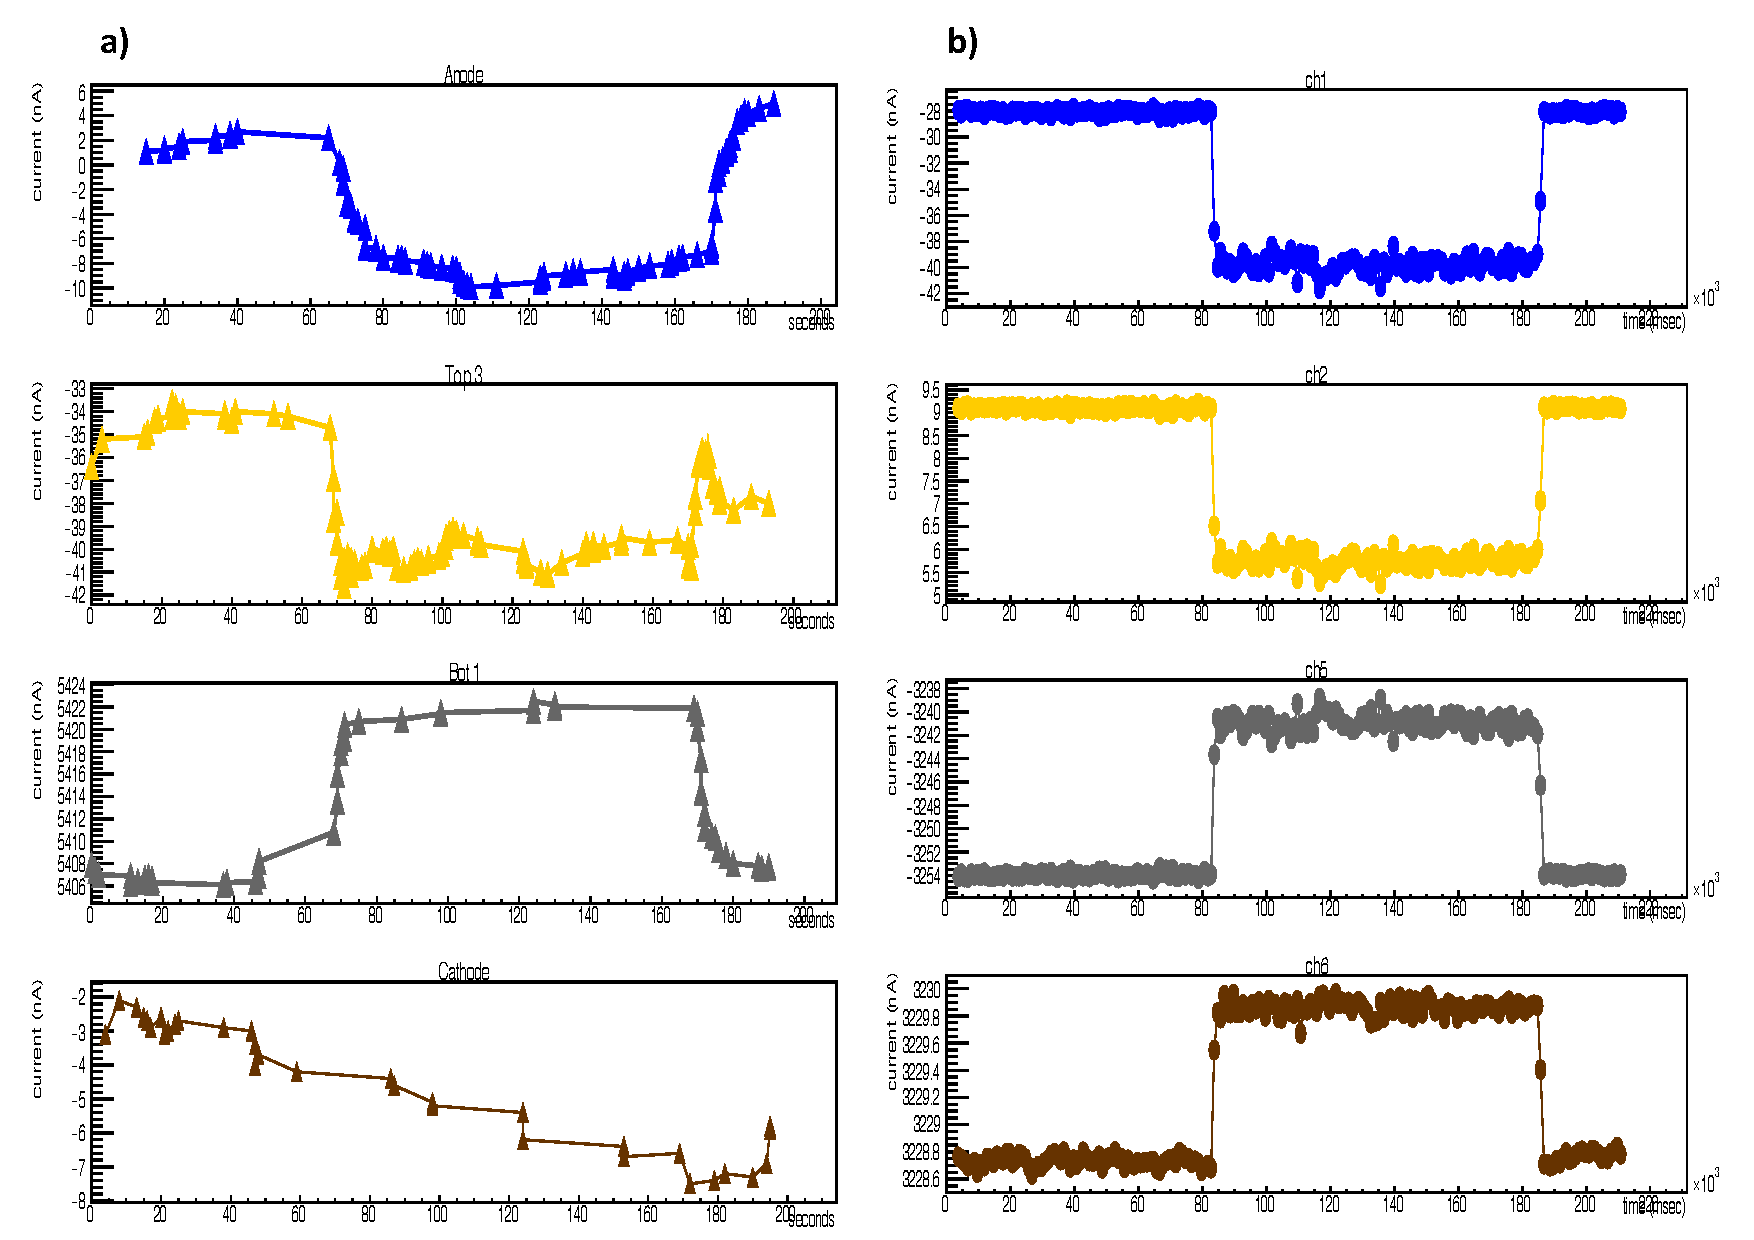
\includegraphics[width=1\textwidth]{Immagini/run190_CAEN_pico.pdf}
	\caption{Anode, Top3, Bot1 and Cathode currents measured with CAEN system a) and PICO b).}
	\label{fig:run190_CAEN_pico}
\end{figure}
\begin{figure}
	\centering
	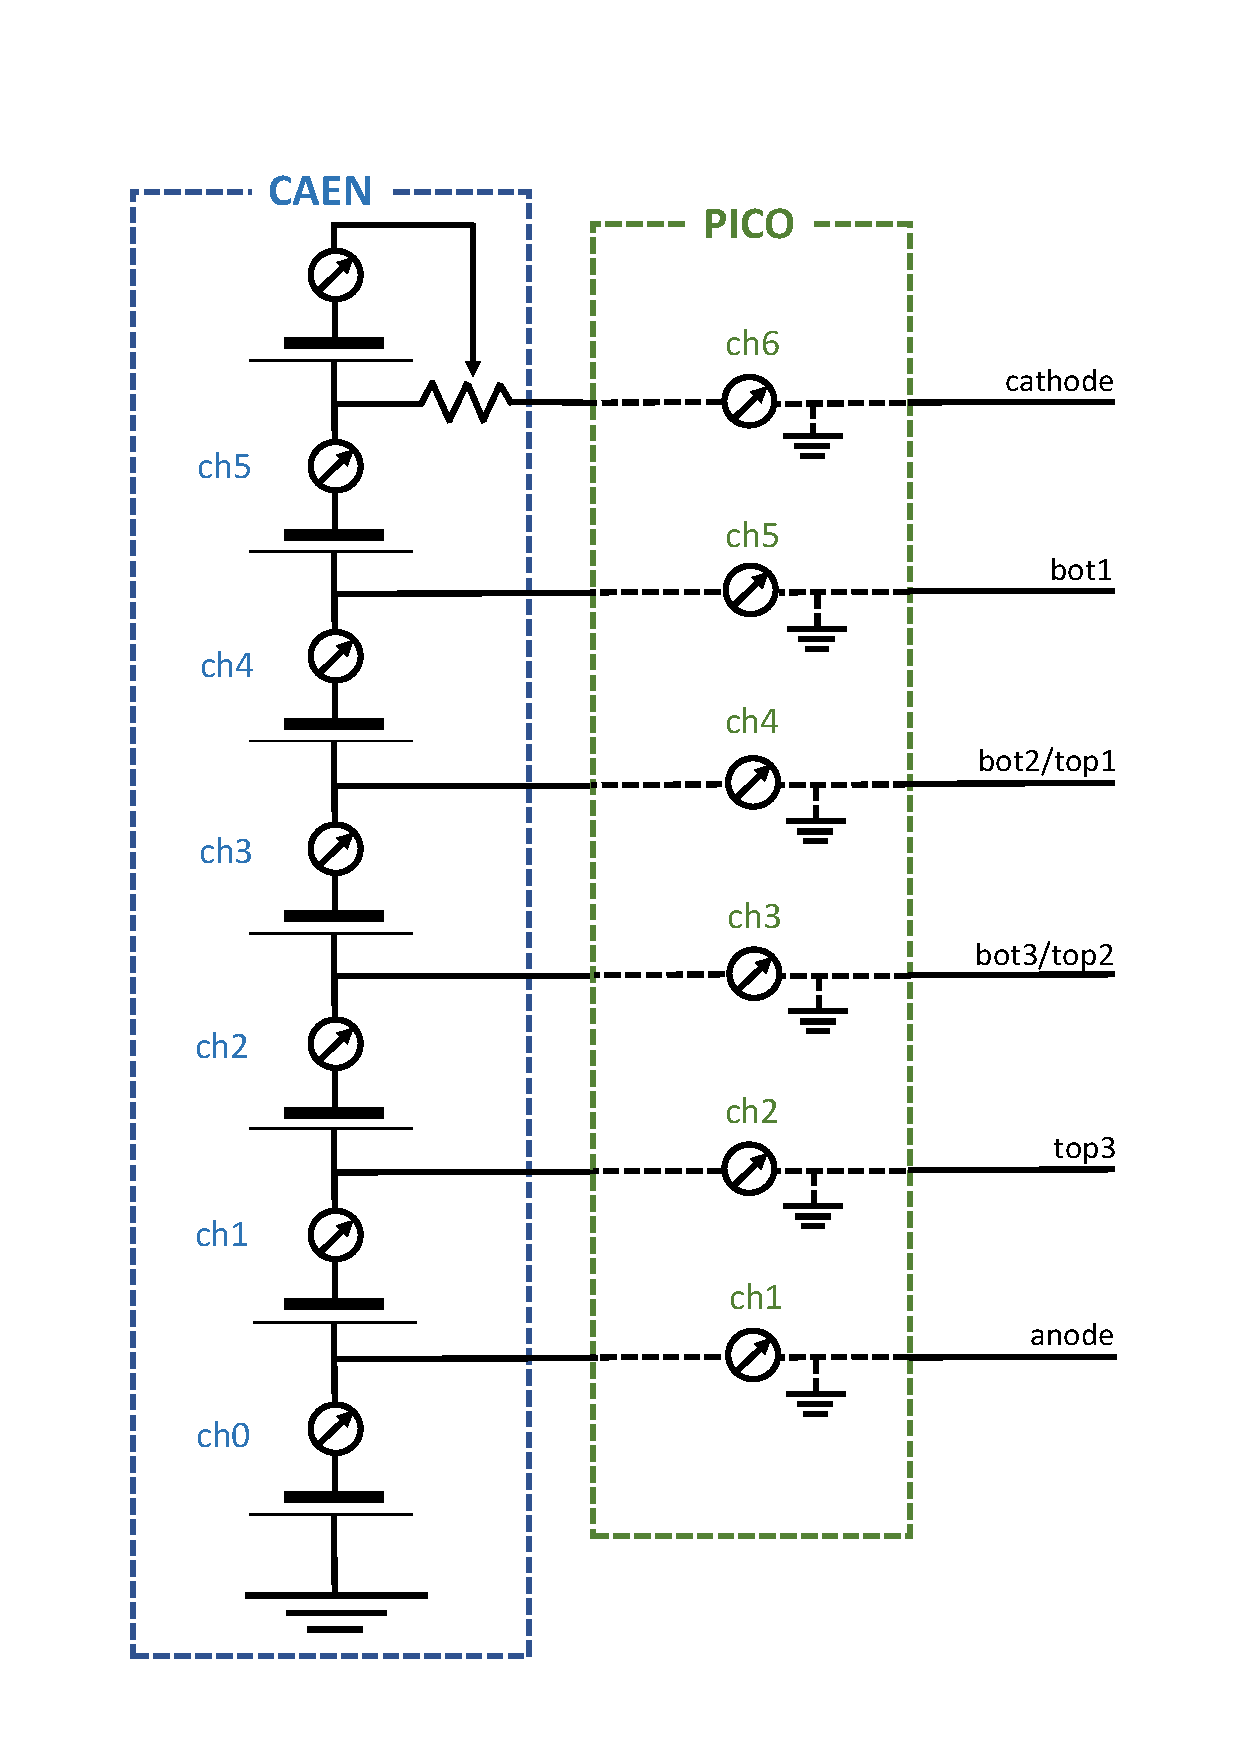
\includegraphics[width=0.8\textwidth]{Immagini/schema_canali.pdf}
	\caption{Current readng scheme for the two ammeters.}
	\label{fig:schema_canali}
\end{figure}

%aggiungere sezione sul sistema da vuoto

\subsection{Tracker prototype}

The tracker prototype consists in a single module (one of the 8 final modules) of reduced size of 100$\times$185$\times$108 mm$^{3}$. This prototype has the same structure as the final FPD but is smaller just in the dispersive direction.\\
The drift region, delimited by the cathode and the multiplication stage, is designed to set a uniform electric field of about 50 V/cm. The drift region is filled with gas at low pressure (10-100 mbar). The gas filling the drift region should have a high drift velocity in order to guarantee a fast collection of the charge and should manifest a saturation of the drift velocity with the electrical field applied.\\
The multiplication stage is based on THGEM foils, described in the next subsection.\\
The induction region is delimited by the anode. The electron cloud emerging from the multiplication region foil are directed towards a first layer of 750 m pitch strips, corresponding to a capacitance of 22 pF. The shaped signal is compared to a suitable threshold and the logic high output of the comparator identifies the hit strip.\\
A scheme of the setup is shown in Figure~\ref{fig:schema_apparato_2}.\\

\begin{figure}
	\centering
	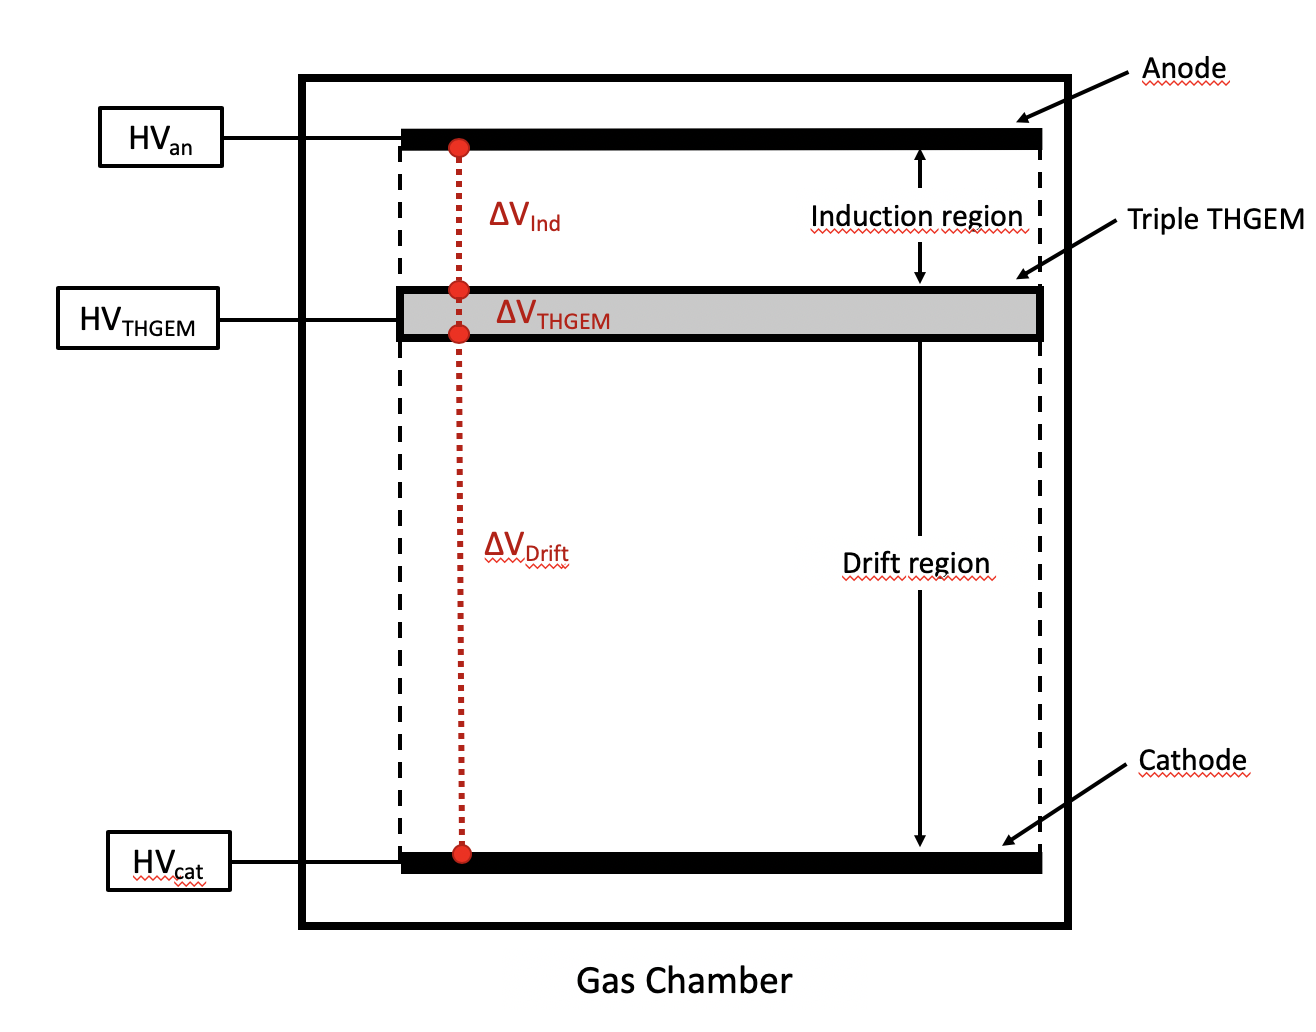
\includegraphics[width=0.9\textwidth]{Immagini/schema_apparato_2.png}
	\caption{The experimental setup.}
	\label{fig:schema_apparato_2}
\end{figure}

\subsection{THGEM}

The two THGEM prototypes are both multiple THGEM, composed by three layers of THGEM, but they show 
different hole pattern for the multiplication.\\
In the first one, referred to as FULL THGEM \textbf{F10} (Figure~\ref{fig:full_thgem}), the holes 
are uniformly distributed over the active surface; in the second one, called ROW THGEM \textbf{R1} 
(Figure~\ref{fig:row_thgem}), the holes are arranged in five rows.\\
The main characteristics of the two prototypes are shown in Table~\ref{tab:thgem}.\\

\begin{table} [b!]
	\begin{center}
		\renewcommand{\arraystretch}{1.2}
\begin{tabular}{|c|c|c|}
\hline 
\textbf{Name} & \textbf{F10} & \textbf{R1} \\ 
\hline 
Substrate material & Ceramic SD103K & PCB  \\ 
\hline 
Finish board thickness [mm] & 1.4 $\pm$ 0.1 & 1.28 \\ 
\hline 
Dimension [$\mbox{mm}^2$] & 107$\times$107 & 107$\times$107 \\ 
\hline 
Rim size [mm] & 0.1 & 0.2  \\ 
\hline  
Rows & 143$\times$143 & 5 \\ 
\hline 
Holes & 20449 & 143 \\ 
\hline 
Hole diameter [mm] & 0.30 $\pm$ 0.05 & 0.280 \\ 
\hline
Hole spacing & 0.75 & 0.75 \\ 
\hline
\end{tabular} 
	\end{center}
	\caption{The main characteristics of the two type of THGEM tested.} \label{tab:thgem}
\end{table}

\begin{figure}
	\centering
		\subfigure[]{\label{fig:full_thgem}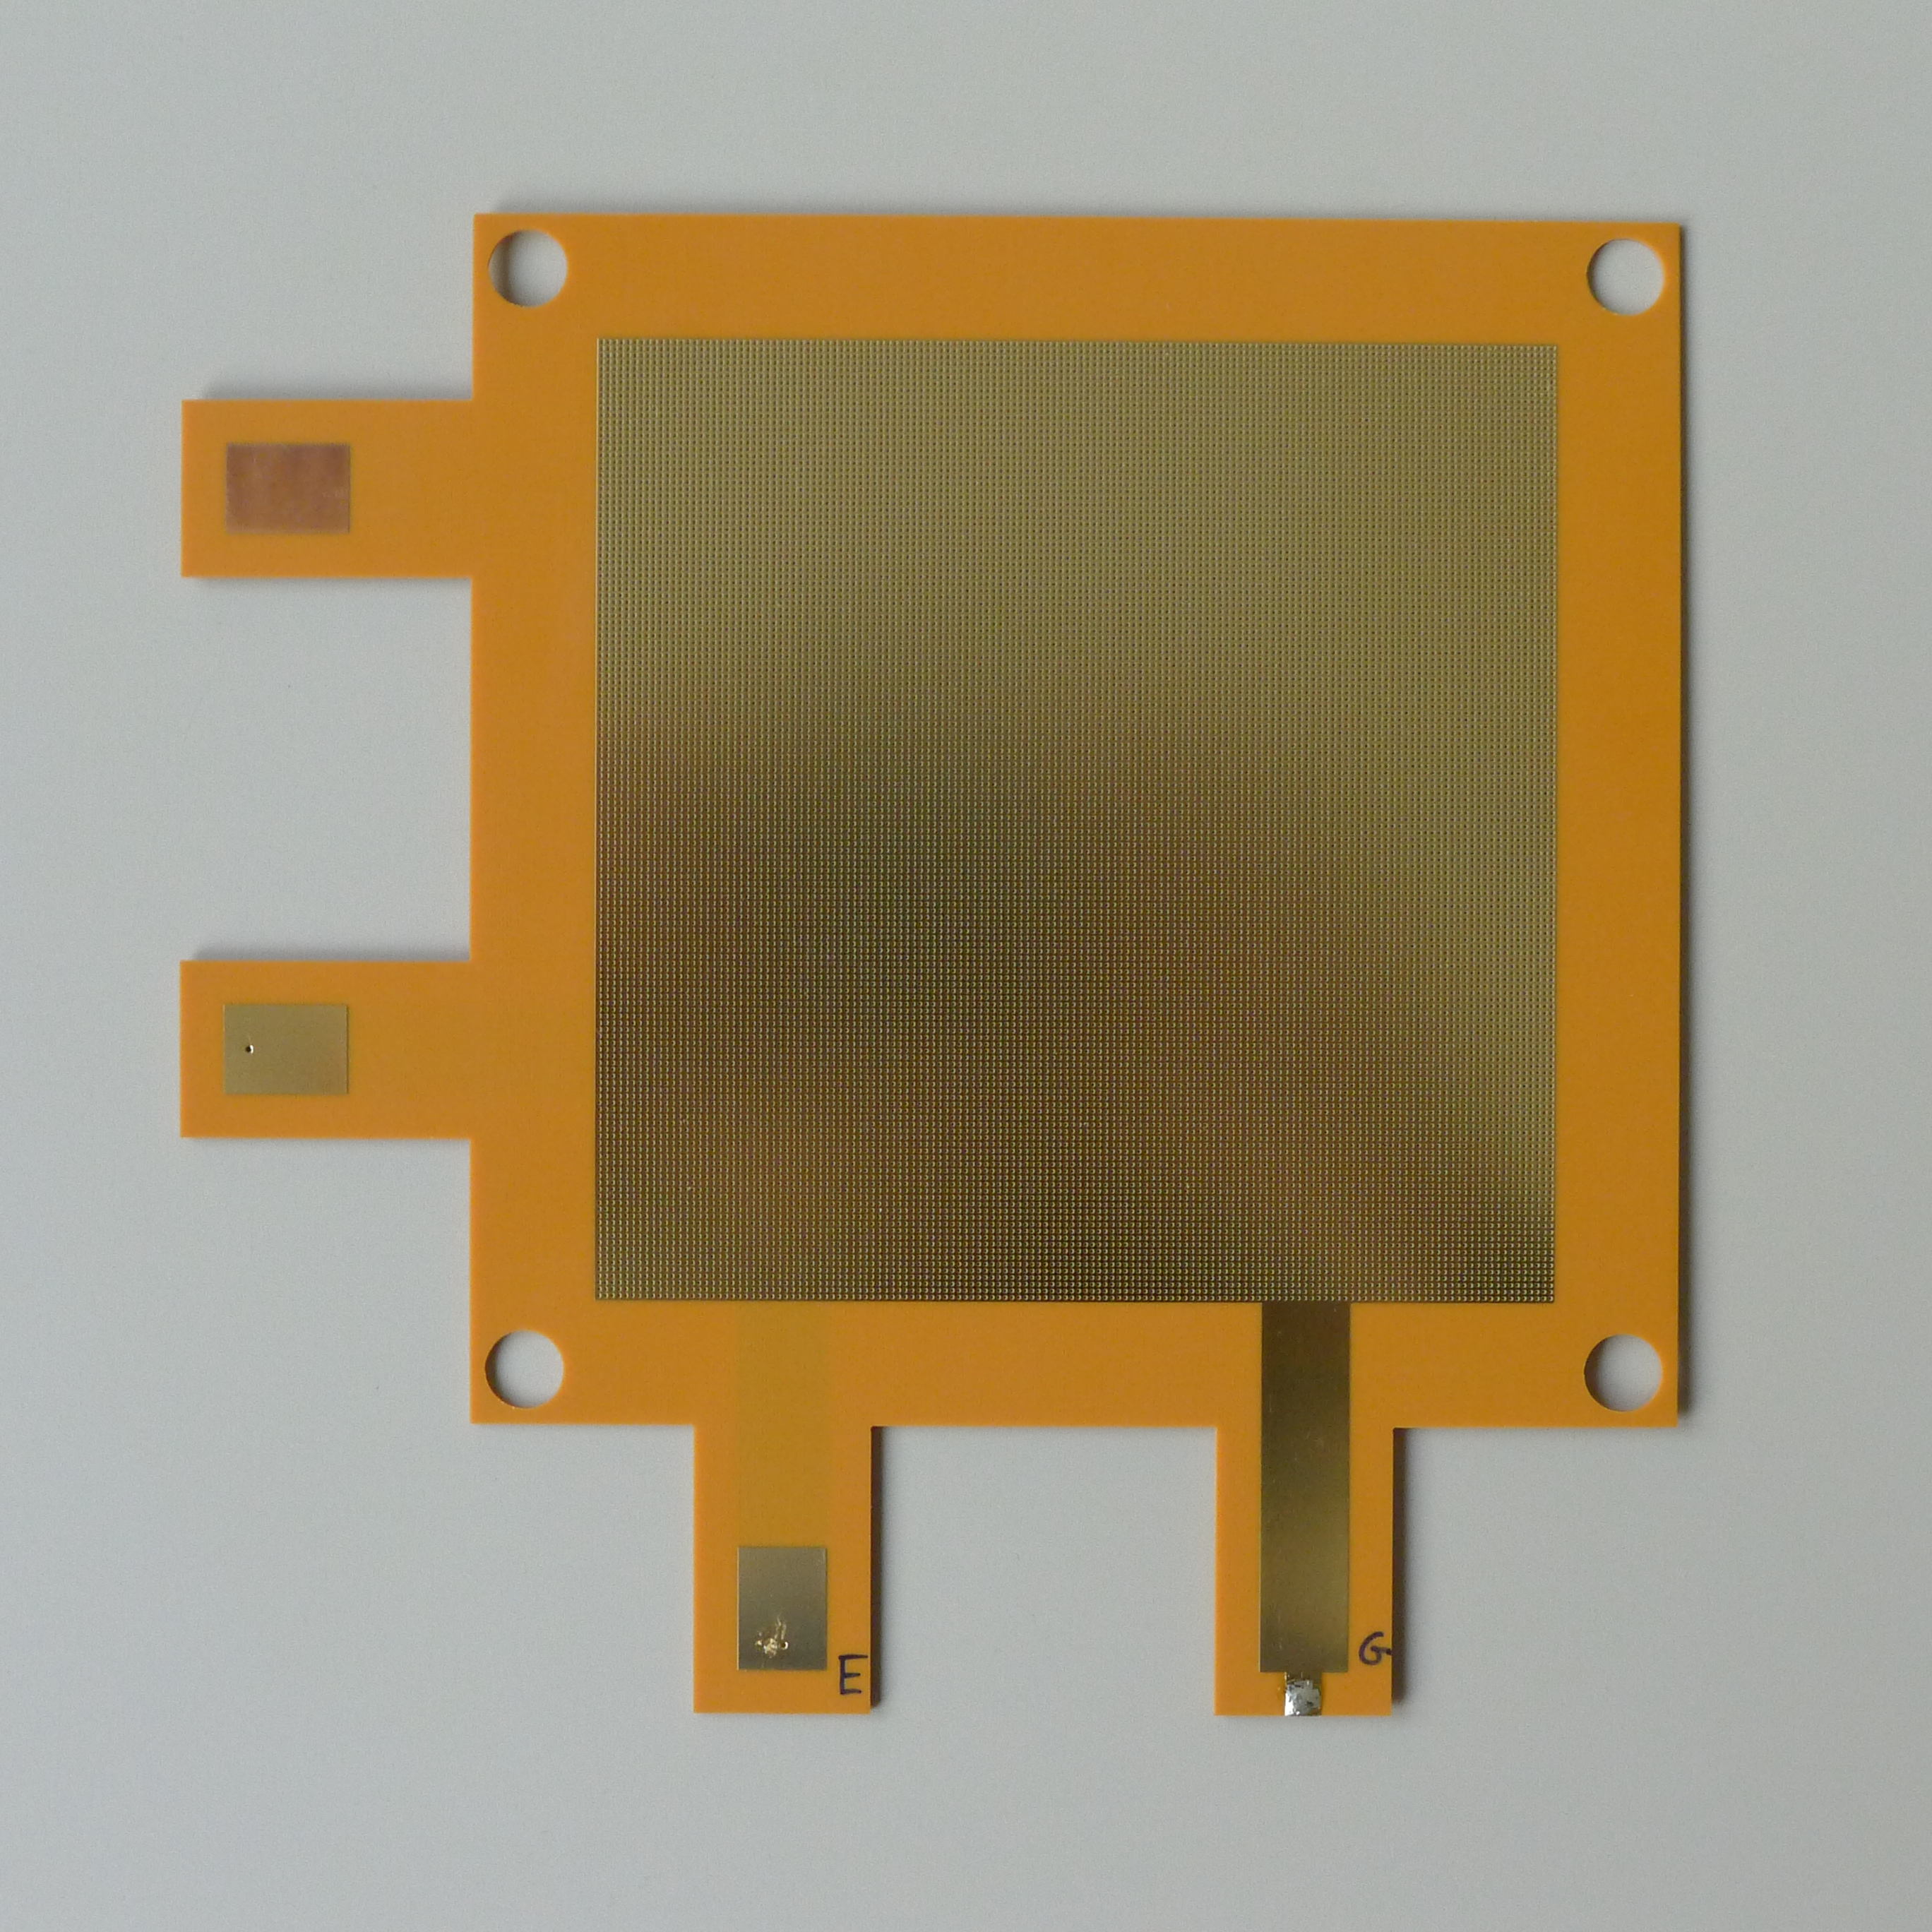
\includegraphics[width=0.45\textwidth]{Immagini/full_thgem.JPG}}
		\hspace{5pt}
		\subfigure[]{\label{fig:full_thgem_holes}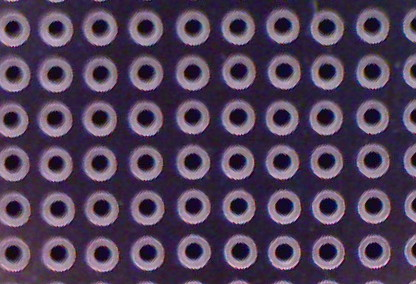
\includegraphics[width=0.45\textwidth]{Immagini/full_thgem_holes.JPG}}
	\caption{In (a) the FULL THGEM prototype, in (b) its hole pattern.}
	\label{fig:full_thgem_complessiva}		
\end{figure}

\begin{figure}
	\centering
	\subfigure[]{\label{fig:row_thgem}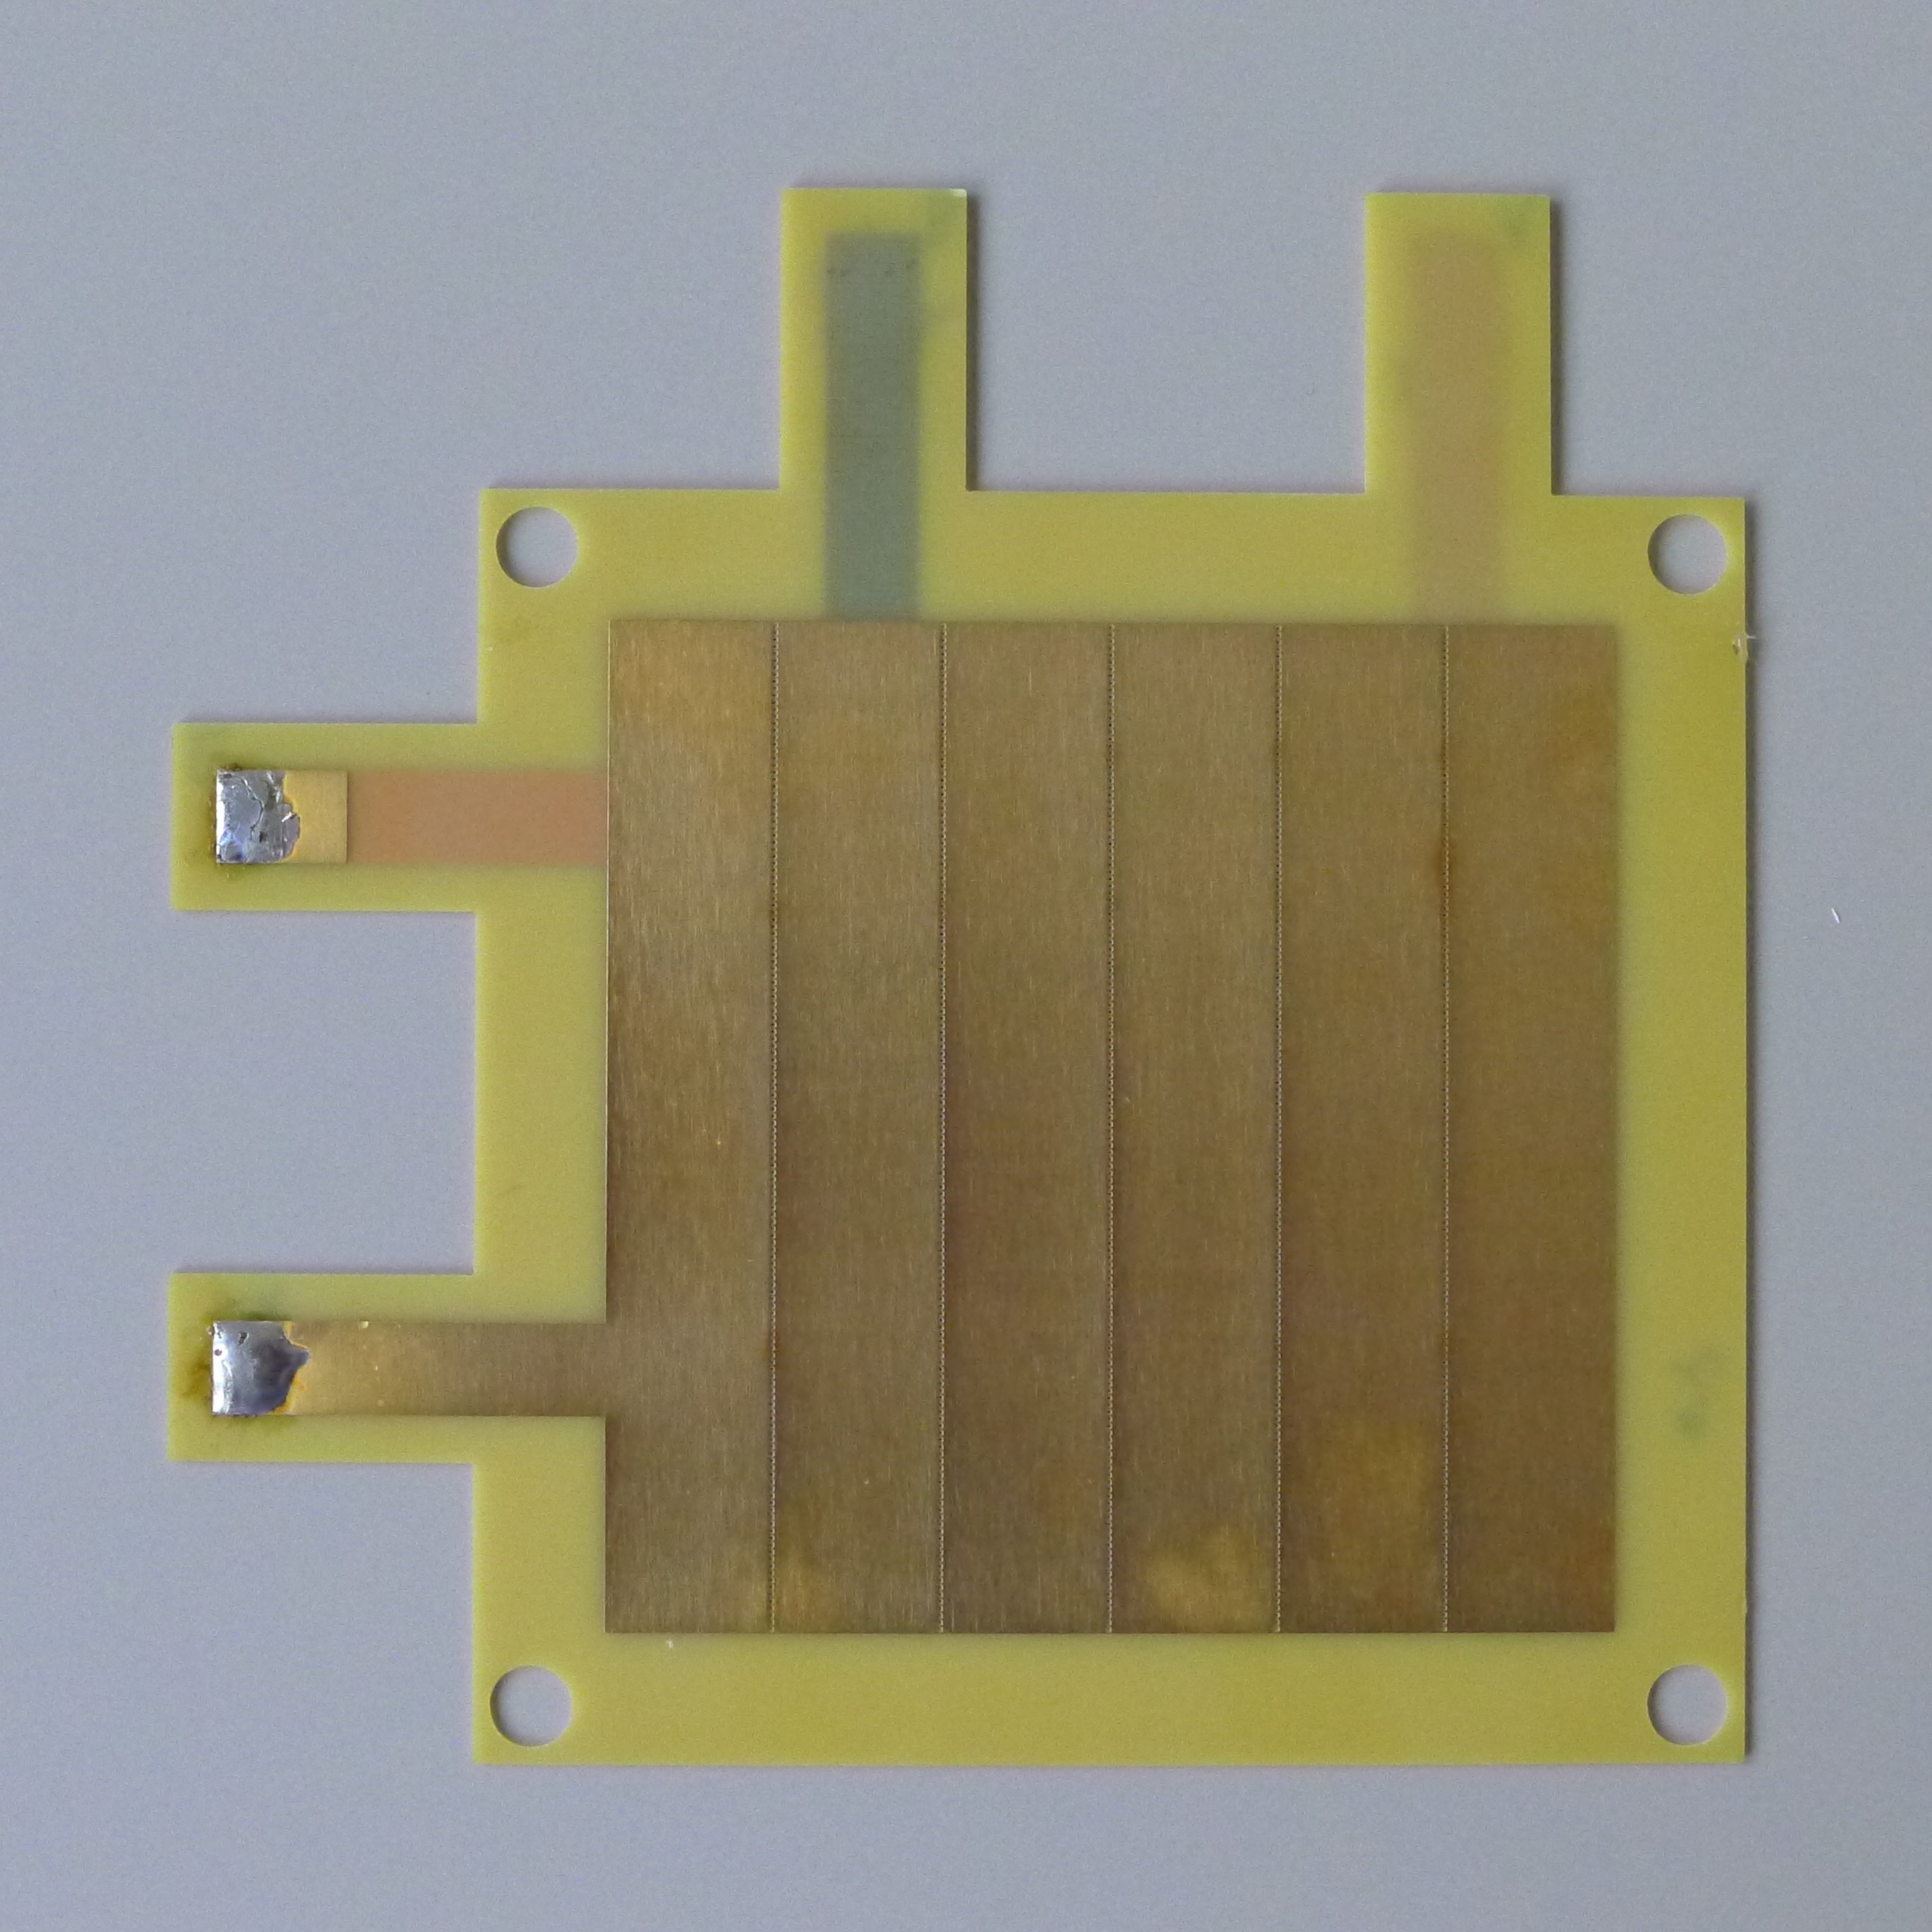
\includegraphics[width=0.45\textwidth]{Immagini/row_thgem.JPG}}
	\hspace{5pt}
	\subfigure[]{\label{fig:row_thgem_holes}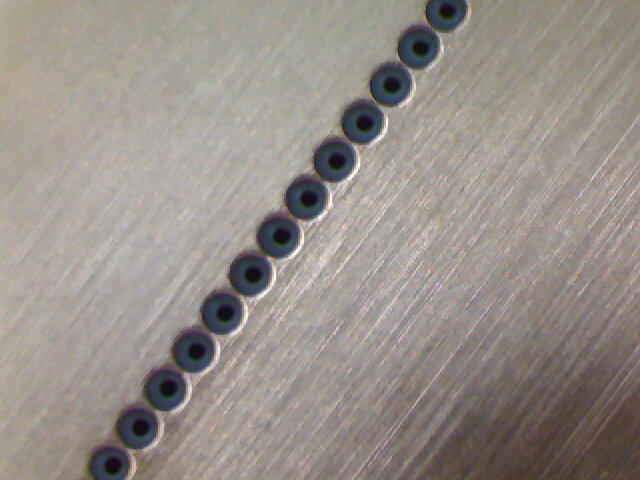
\includegraphics[width=0.45\textwidth]{Immagini/row_thgem_holes.JPG}}
	\caption{In (a) the ROW THGEM prototype, in (b) its hole pattern.}
	\label{fig:row_thgem_complessiva}		
\end{figure}

\section{Method}

The main parameters that define the behaviour of the detector are: gas pressure, voltage of the THGEM (V$_{THGEM}$),
voltage of the induction region (V$_{ind}$) and coltage of the drfit region (V$_{drift}$).

The method consists in keeping fix all the parameter but one and to measure all the currents of all the
electrodes varying just one of the parameters.
For example we kepp fix the gas pressure the V$_{drift}$), V$_{ind}$), whle the V$_{THGEM}$) was
changed a small step. In this way we get 6 plot currents as a functio of V$_{THGEM}$).

In order to measure with the CAEN ammeter the current on the Anode, it cannot be kept at ground
therefore its voltage was fixed to an arbitrary value of 20~V that should not affect the 
measurements of the currents of any electrodes. 
During induction scan THGEM and drift voltages 
were fixed and anode, bot1, top3 and cathode currents were acquired (see 
Figure~\ref{fig:schema_canali}). When THGEM voltage was scanned induction and drift voltages were fixed and the same currents were acquired. Changing drift voltage value induction and THGEM voltages were fixed and the fourth currents were acquired.\\
A run lasts usually 180 s;\\
60 s with shutter closed;\\
90 s with shutter open;\\
30 s with shutter closed.\\
An average of the current flowing during the first 60 s (shutter closed) and an average during
the 90 s with shutter open is performed.
The difference between the two measurements with shutter open and closed give
 the actual current associated to the $\alpha$-particles entering the detector.
In this way any dark current coming from the detector or from the ammeter is subtracted\footnote{A possible source of
dark current is due to the X-ray produced by the $\alpha$-source that are not stopped by the shutter.}.\\

\clearpage

\section{Measurements}

%i canali 3 e 4 possono essere ignorati perche non danno mai segnale

%spieghiamo i diversi scan (induzione, thgem e drift)

%In this section the results of 

%For the sake of clarity

\subsection{FULL THGEM}

\subsubsection{Scan on \Vind}

%The scan on \Vind aimed at studying the behaviour of 

%A preliminary study of \Vind{} variation effects on the measured currents has been done at several pressure and setting different \Vthgem{} and \Vdrift{} values.
A series of systematic measurements were conducted to study the effects of the variation of the potential difference \Vind{} on the measured currents.
These measurements were done fixing three different pressure (P) and setting suitable values of \Vthgem{} and \Vdrift.
A summary scheme of the adopted configurations is shown in Table~\ref{tab:FULLTHGEM_vind}.
\begin{table} [b!]
	\begin{center}
		\renewcommand{\arraystretch}{1.2}
		\begin{tabular} {ccccc}
			P (mbar) & & \Vthgem{} (V) & & \Vdrift{} (V)\\
			\toprule[0.1em]
			%\hline
			30	& &	220	& &	1000 \\
			30	& &	200	& &	1000 \\
			30	& &	230	& &	1000 \\
			20	& &	200	& & 1000 \\
			11	& & 170	& & 600 \\
			
			\bottomrule[0.1em]
		\end{tabular}
	\end{center}
	\caption{The values of pressure (P), \Vthgem{} and \Vdrift{} adopted for the study on \Vind.} \label{tab:FULLTHGEM_vind}
\end{table}
%\begin{table} [b!]
%	\begin{center}
%		\renewcommand{\arraystretch}{1.2}
%		\begin{tabular} {ccccccc}
%			P (mbar) & & \Vthgem{} (V) & & \Vdrift{} (V) & & optimal \Vind{} (V) \\
%			\toprule[0.1em]
%			%\hline
%			30	& &	220	& &	1000 & & 120 \\
%			30	& &	200	& &	1000 & &  \\
%			30	& &	230	& &	1000 & & \\
%			20	& &	200	& & 1000 & & \\
%			11	& & 170	& & 600  & &\\
%			
%			\bottomrule[0.1em]
%		\end{tabular}
%	\end{center}
%	\caption{The values of pressure (P), \Vthgem{} and \Vdrift{} adopted for the study on \Vind.} \label{tab:FULLTHGEM_vind}
%\end{table}
The \Vind{} scans were carried out starting from 0~V and increasing the voltage by 10 or 20~V per run, until the discharge value is reached.
This value is dependent on the gas pressure and the values set for \Vthgem{} and \Vdrift: for P~=~30~mbar it was 220~V, for P~=~20~mbar it was 200~V, and for P~=~11~mbar it was 150~V.


The result of the scan at 30~mbar and with \Vthgem{}~=~220~V is shown in Figure~\ref{fig:induction_FULLTHGEM_30mbar}: by raising the value of \Vind{}, the anodic current (blue line) increases, while the top3 current (yellow line) approaches to zero.
\begin{figure}[!t]
	\centering
	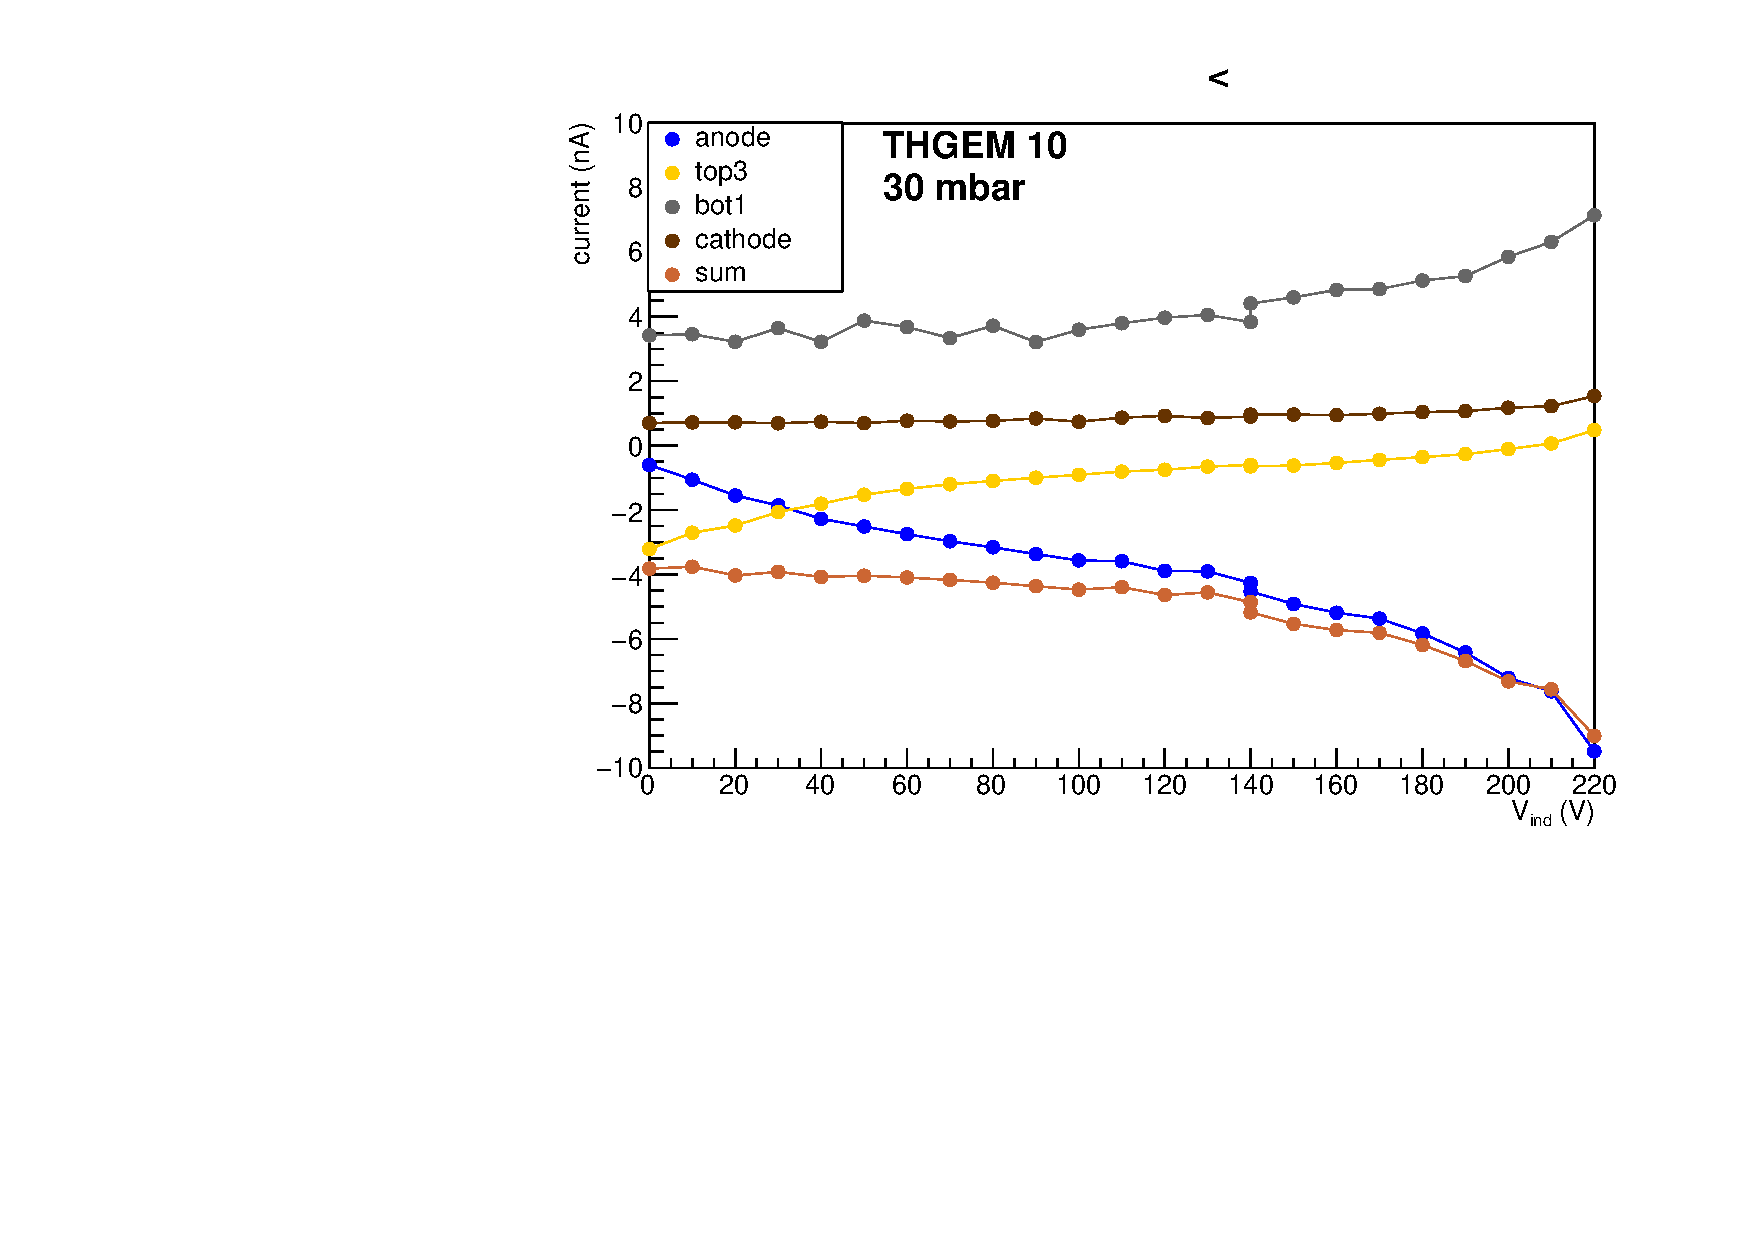
\includegraphics[width=\textwidth]{Immagini/inductionScan_THGEM10_30mbar.pdf}
	\caption{Currents measured during the scan on the voltage \Vind{} across the induction region at 30~mbar and with \Vthgem{}~=~220~V.}
	\label{fig:induction_FULLTHGEM_30mbar}
\end{figure}
Up to 140~V, their change is such that their sum (orange line) is constant.
% but their change is such that their sum (orange line) is constant.
%Up to 140~V, when \Vind{} increases, the anodic current (blue line) goes up, the top3 current (yellow line) approaches to zero, and their sum (orange line) is constant.
This means that the stronger is the electric field in the induction region, the greater is the fraction of secondary electrons collected at the anode.
%Up to 140~V, the sum of anode and top3 currents (orange line) is constant, so the 
%The total number of secondary electrons, 
%The sum of anode and top3 currents is constant 
%; in particular, for \Vind{} greater than about 30~V most electrons
%This means that when the electric field in the induction region is weak, most of the electrons produced by multiplication are collected at the top3 electrode and only a few reaches the anode.
For \Vind{} greater than 140~V, the anode and top3 currents sum increases: this behaviour can be explained considering that, when the voltage is high enough, the multiplication region extends out of the THGEM holes, occupying a section of the induction region.
The concomitant increase of the bot3 current may confirm this hypothesis.
For \Vind{} equal to 220~V, the top3 current becomes positive, so that some ions are collected at the top3 electrode.
For these values of pressure, \Vthgem{} and \Vdrift, a plateau is reached between 110 and 130~V, where the field pushes almost all the electrons from the avalanche to the anode.
In these conditions, the optimal value of \Vind{} is 120~V.


Keeping the pressure at 30~mbar, other two measurements on \Vind~{} were conducted with \Vthgem{} equal to 200 or 230~V.
The results of these measurements are shown, respectively, in Figure~\ref{fig:induction_FULLTHGEM_30mbar_other_VTHGEM_a} and ~\ref{fig:induction_FULLTHGEM_30mbar_other_VTHGEM_b}.
\begin{figure}[!htb]
	\centering
	\subfigure[]{ \label{fig:induction_FULLTHGEM_30mbar_other_VTHGEM_a} 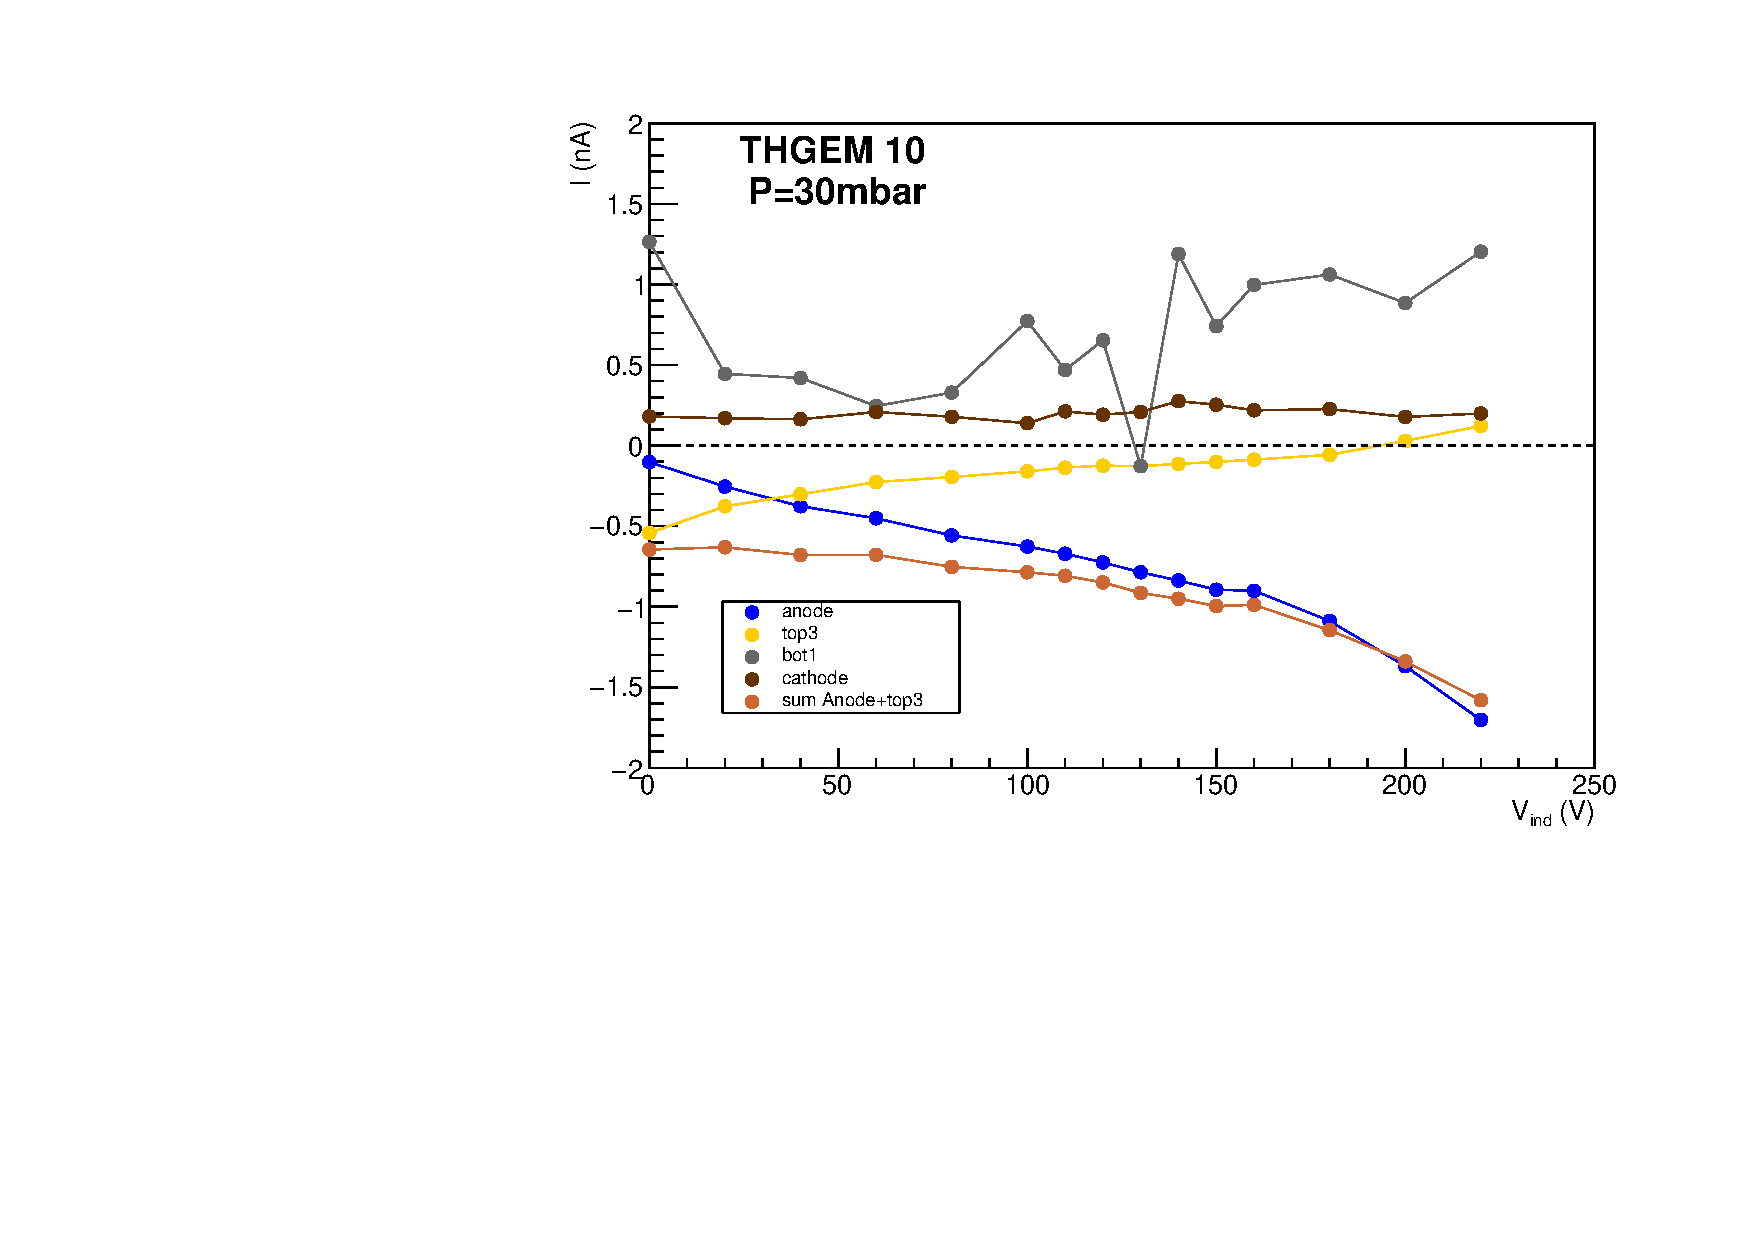
\includegraphics[width=0.96\textwidth]{Immagini/inductionScan_THGEM10_30mbar_bis.pdf}}
	\subfigure[]{ 	\label{fig:induction_FULLTHGEM_30mbar_other_VTHGEM_b} 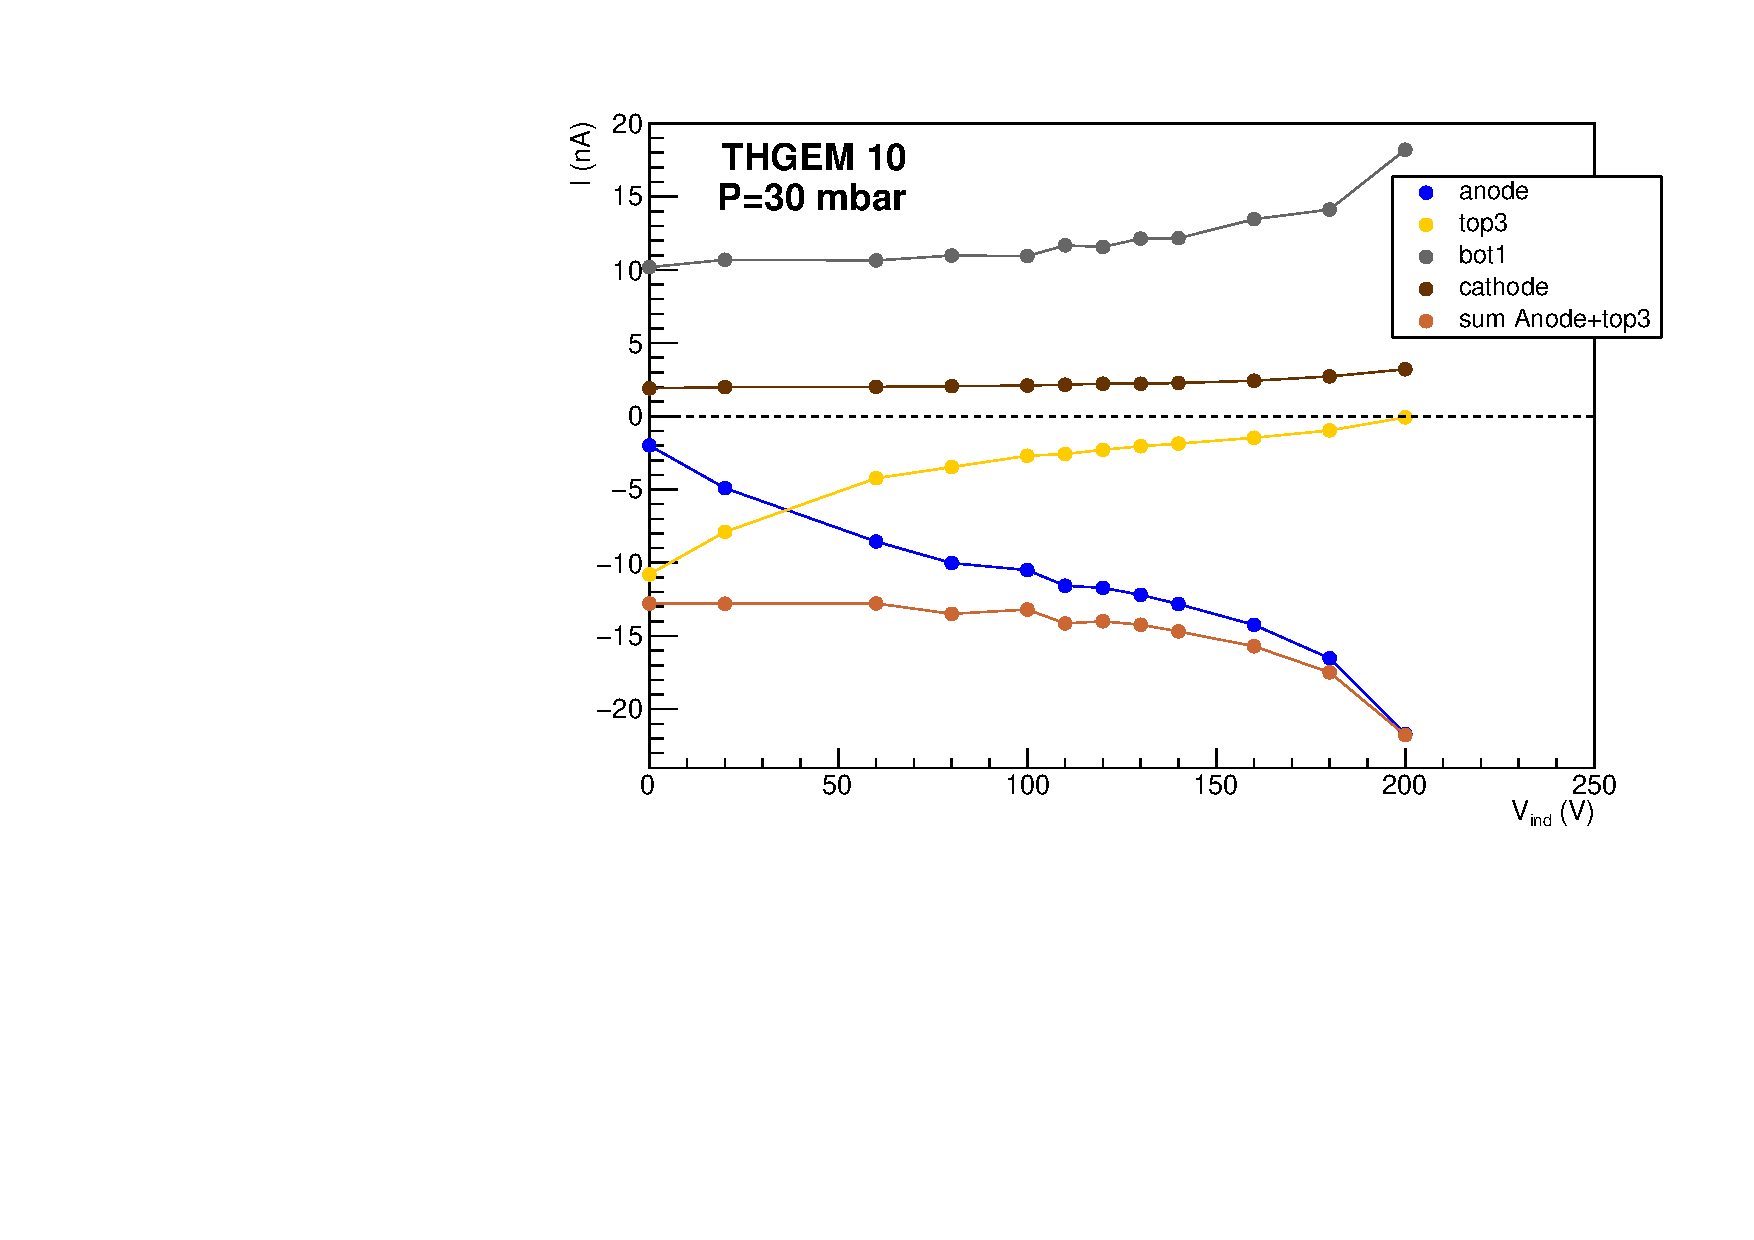
\includegraphics[width=0.96\textwidth]{Immagini/inductionScan_THGEM10_30mbar_tris.pdf}}
	\caption{Currents measured during the scan on the voltage \Vind{} across the induction region at 30~mbar: in (a) for \Vthgem~=~200~V, in (b) for \Vthgem~=~230~V.}
	\label{fig:induction_FULLTHGEM_30mbar_other_VTHGEM}
\end{figure}
The comparison between these two figures makes apparent that the magnitude of the measured currents increases with increasing \Vthgem, because the multiplication factor goes up.
Most considerations made in the case with \Vthgem~=~220~V are also valid for these two measurements, except that the plateau region is less evident or absent.
For \Vthgem~=~200~V the bot1 current fluctuations are due to the lower accuracy of the corresponding PICO channel.


The result of the tests at 20 and 11~mbar are, respectively, shown in Figure~\ref{fig:induction_FULLTHGEM_20mbar} and~\ref{fig:induction_FULLTHGEM_11mbar}.
In the former case there is not a clear plateau region, but the suggested operative voltage range is between 90 and 120~V.
For P~=~20~mbar the optimal \Vind{} value is 100~V.
In the latter case a plateau region is visible from 0 to 80~V, so the optimal \Vind{} value is 70~V.
In both cases the cross point between the anode and the top3 currents is at about 30~V and the top3 current becomes positive for high \Vind{} values.



\begin{figure}[!htb]
	\centering
	\subfigure[]{ \label{fig:induction_FULLTHGEM_20mbar} 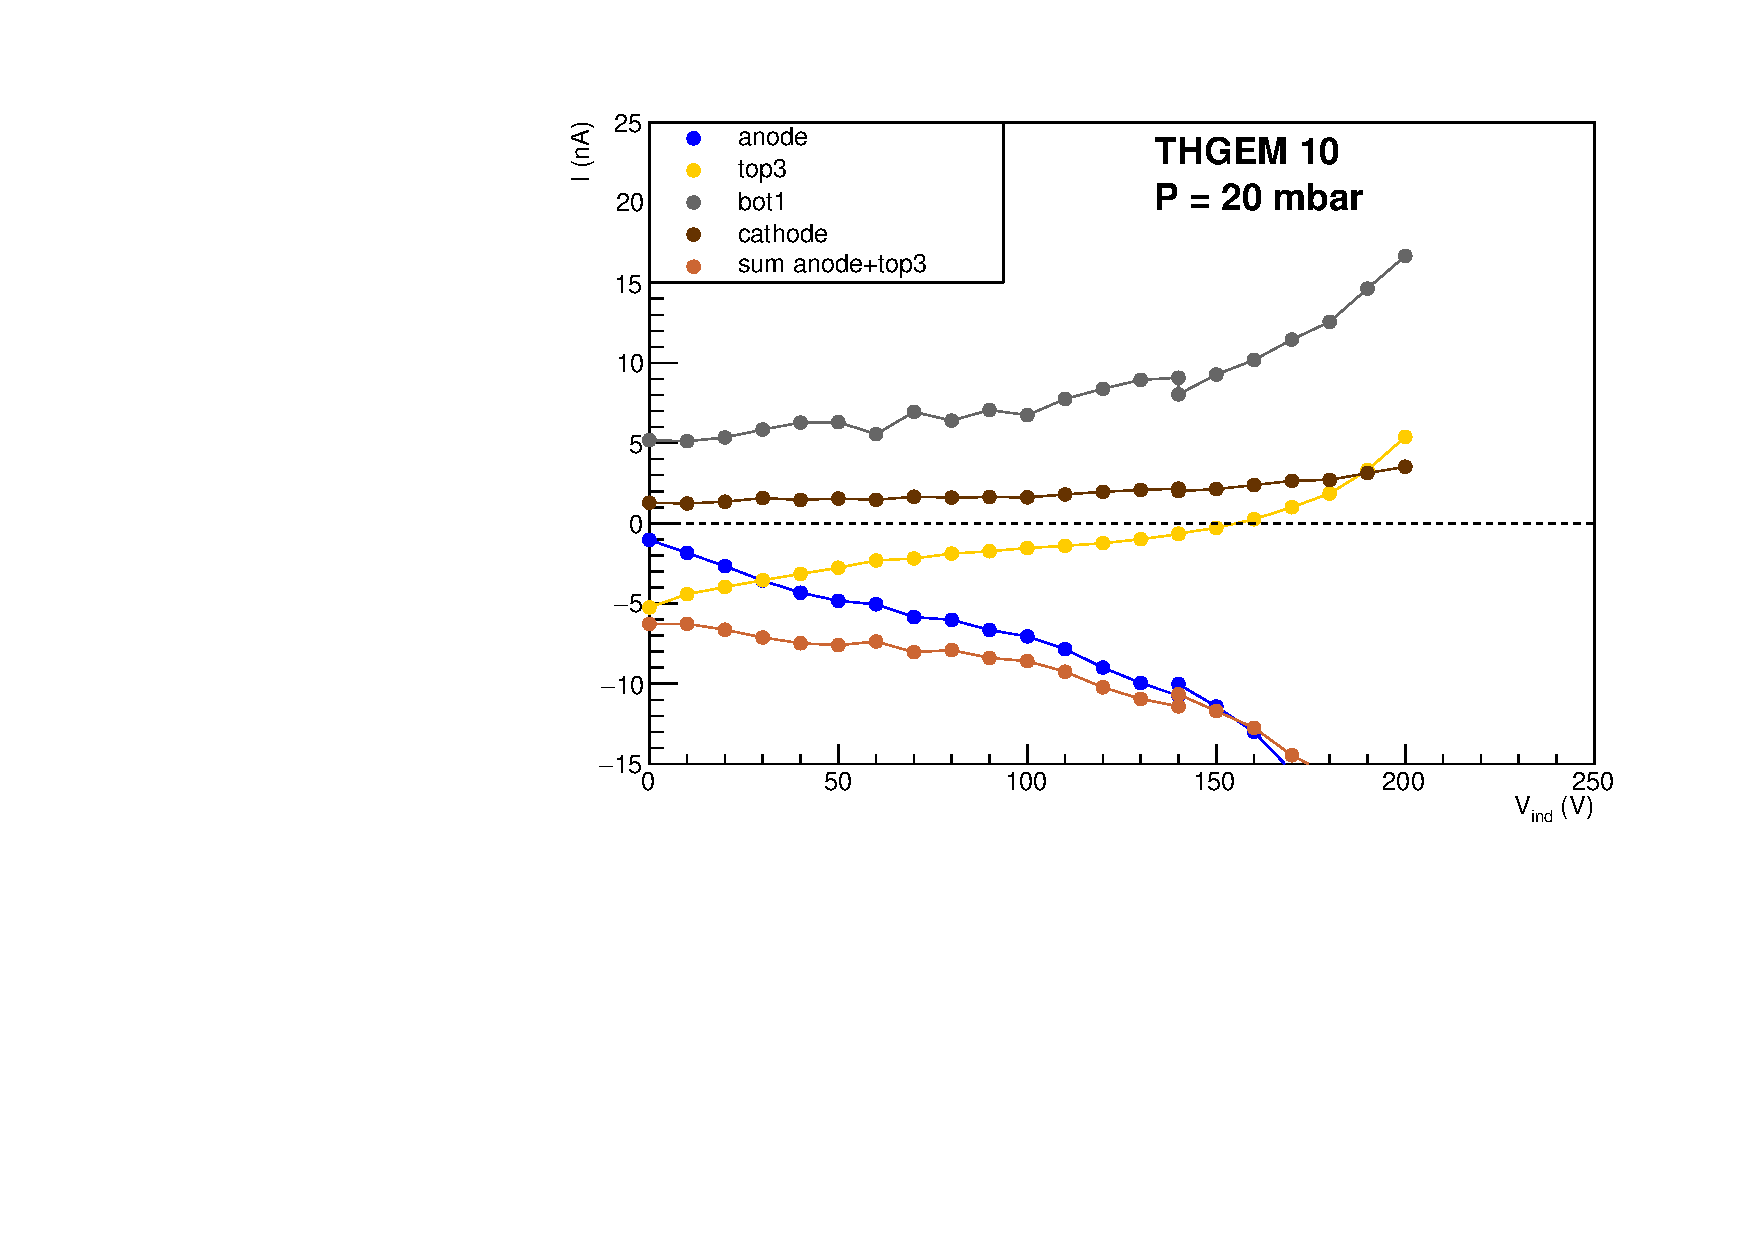
\includegraphics[width=0.97\textwidth]{Immagini/inductionScan_THGEM10_20mbar.pdf}}
	\subfigure[]{ 	\label{fig:induction_FULLTHGEM_11mbar} \includegraphics[width=0.97\textwidth]{Immagini/inductionScan_THGEM10_10mbar_tris.pdf}}
	\caption{Currents measured during the scan on the voltage \Vind{} across the induction region: in (a) at 20~mbar, in (b) at 11~mbar.}
	\label{fig:induction_FULLTHGEM_other_pressure}
\end{figure}

%Also in these two measurements, when \Vind{} increases, the anodic current increases, while the top3 current decreases. The crossing point of these two currents is still at around 32~V. After a certain value the sum of the anode and top3 current varies rapidly.

%The effects seen for \Vthgem~=~220~V appear as well in these two cases.
%The magnitude of the measured currents increases with increasing \Vthgem, because
%For \Vthgem~=~200~V the magnitude of the measured currents is lower than in the previous case, while for \Vthgem~=~230~V it is 

%as expected, increasing \Vind{} the fraction of electrons collected at the anode
%this plot displays some of the most important features



%\subsubsection*{Scan on induction voltage at 30 mbar}
%To find the optimal value for the induction voltage, a scan on this parameter has been done. The measured currents obtained for a pressure of 30~mbar and for \Vthgem~=~220~V and \Vdrift~=~1000~V are shown in Figure~\ref{fig:induction_FULLTHGEM_30mbar}. In each plot, bot2/top1 and bot3/top2 currents are not shown because their values do not change during the measurement. In Figure~\ref{fig:induction_FULLTHGEM_30mbar} is shown the sum of the anode and top3 currents. This curve has a plateau zone in the range 110$\div$130~V, so the optimal value for the \Vind is 120~V. The induction scan was repeated with \Vthgem~=~200~V and \Vthgem~=~230~V, but there was no visible plateau. In each induction scan, when the set voltage exceeds a certain value (different in the three cases), the sum of anode and top3 currents increases. This behaviour can be explained because the multiplication region extends out of the hole of the THGEM. The electric field gives a further multiplication and some ions reach the THGEM.

\clearpage

\subsubsection{Scan on \Vthgem}

In order to study the multiplication factor of the FULL THGEM in different conditions, a series of measurements was conducted varying the voltage \Vthgem, while pressure, \Vind{} and \Vdrift{} were set to fixed values.
The variation range of \Vthgem{} was determined in this way: the lower extreme is the minimum value at which a variation of the measured currents is visible, while the higher extreme is the discharge value.
The range depends on the selected pressure and on \Vind{} and \Vdrift: for P~=~30 mbar it was from 180 to 235~V, for P~=~20~mbar it was from 150 to 215~V, and for P~=~11~mbar it was from 130 to 210~V.
The increments were ranging from 5 to 10~V.
The chosen values of pressure, \Vind{} and \Vdrift{} are shown in Table~\ref{tab:FULLTHGEM_vthgem}.

\begin{table} [!h]
	\begin{center}
		\renewcommand{\arraystretch}{1.2}
		\begin{tabular} {ccccccc}
			P (mbar) & & \Vind{} (V) & & \Vdrift{} (V) & & \Vthgem{} range (V)\\
			\toprule[0.1em]
			%\hline
			30	& &	120	& &	1000	& & 180$\div$235 \\
			20	& &	100	& & 1000	& & 150$\div$215 \\
			11	& & 70	& & 600		& & 130$\div$210 \\
			
			\bottomrule[0.1em]
		\end{tabular}
	\end{center}
	\caption{The values of pressure, \Vind{} and \Vdrift{} adopted for the study on \Vthgem.} \label{tab:FULLTHGEM_vthgem}
\end{table}

Figure~\ref{fig:thgem_FULLTHGEM_30mbar} displays the result of the measurement at 30~mbar.
As \Vthgem{} increases, the currents show an exponential growth, typical of gas detectors in avalanche regime.
In these conditions, the optimal value of \Vthgem{} is 220~V.
\begin{figure}[!t]
	\centering
	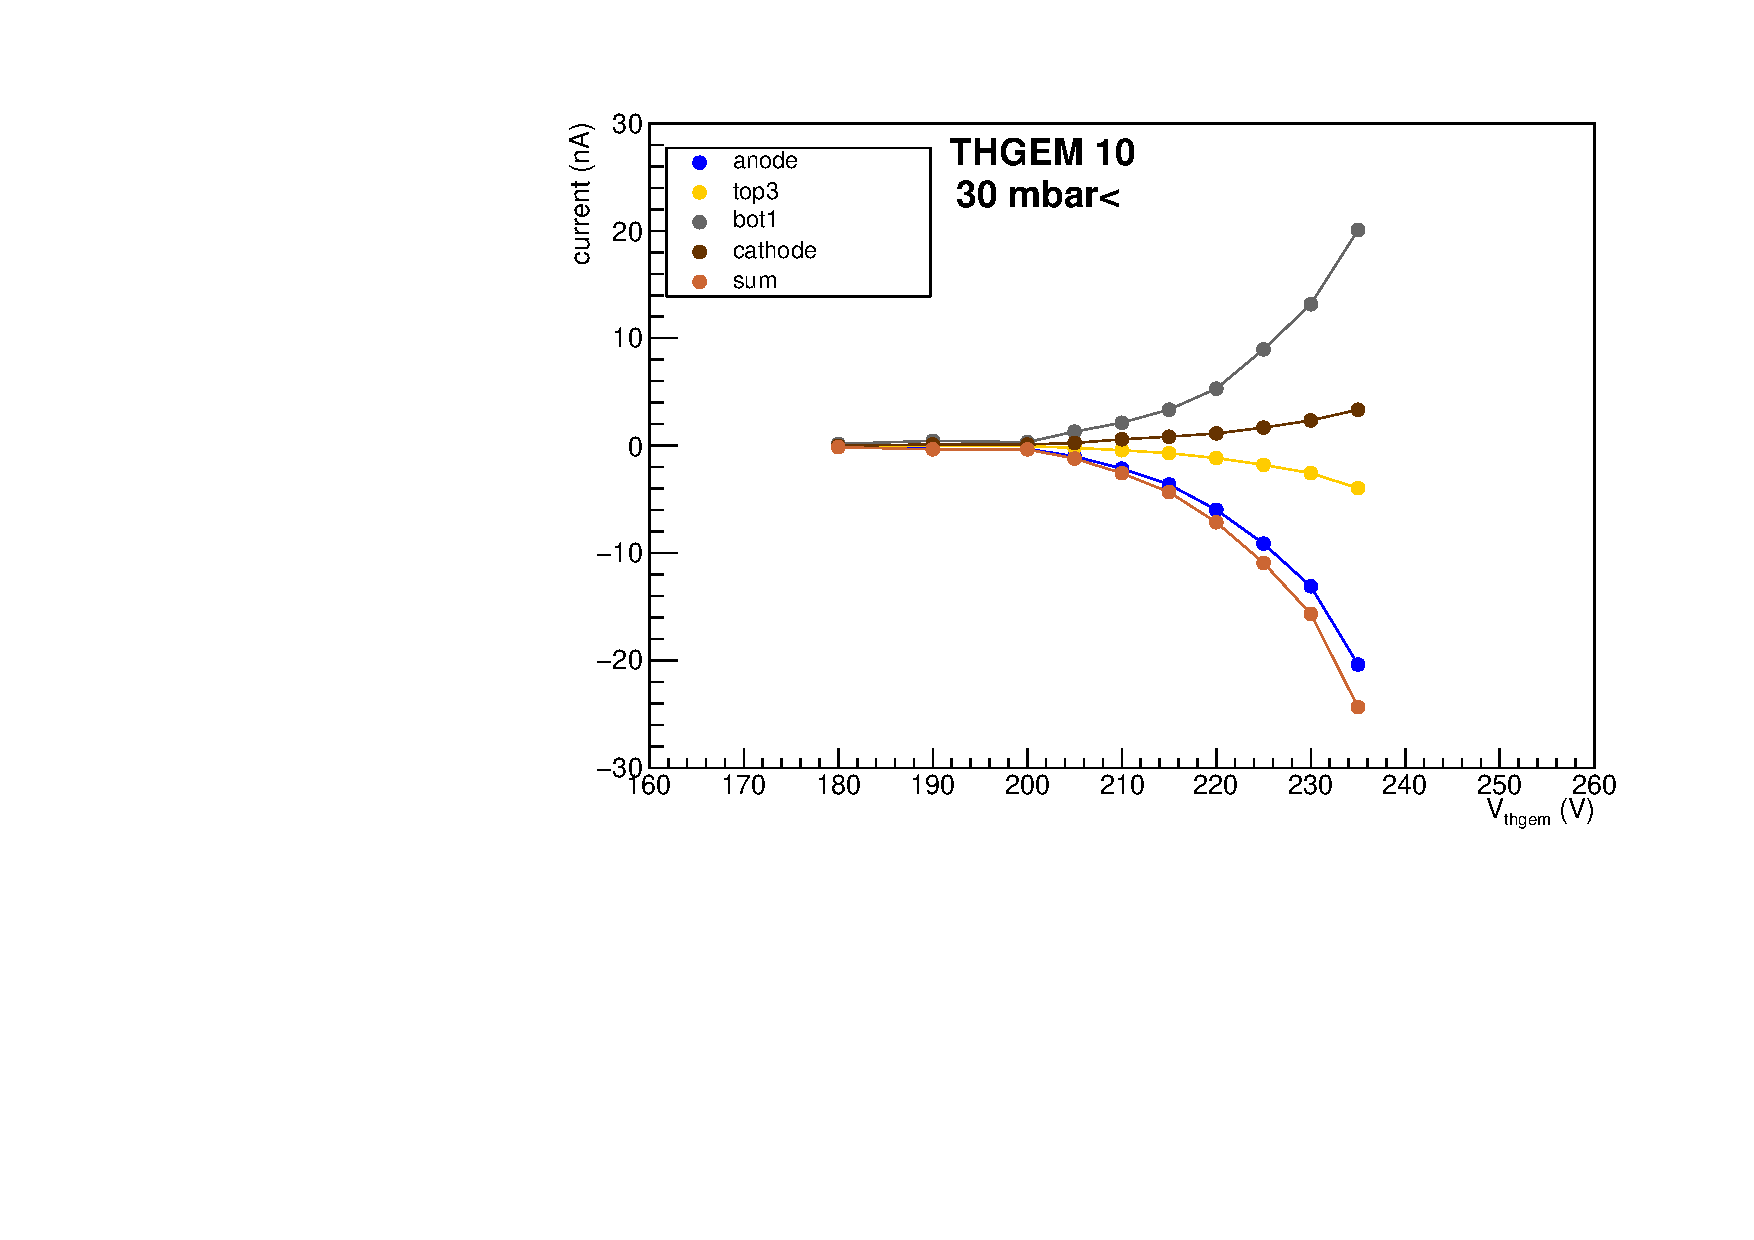
\includegraphics[width=\textwidth]{Immagini/thgemScan_THGEM10_30mbar.pdf}
	\caption{Currents measured during the scan on the voltage \Vthgem{} across each FULL THGEM at 30~mbar.}
	\label{fig:thgem_FULLTHGEM_30mbar}
\end{figure}

The results for P~=~20~mbar and P~=~11~mbar are respectively shown in Figure~\ref{fig:thgem_FULLTHGEM_20mbar} and~\ref{fig:thgem_FULLTHGEM_11mbar}.
In both cases, the measured currents exhibit an exponential behaviour.
The optimal \Vthgem{} value for P~=~20~mbar is 205~V, while for P~=~11~mbar it is 190~V.

\begin{figure}[!htb]
	\centering
	\subfigure[]{ \label{fig:thgem_FULLTHGEM_20mbar} 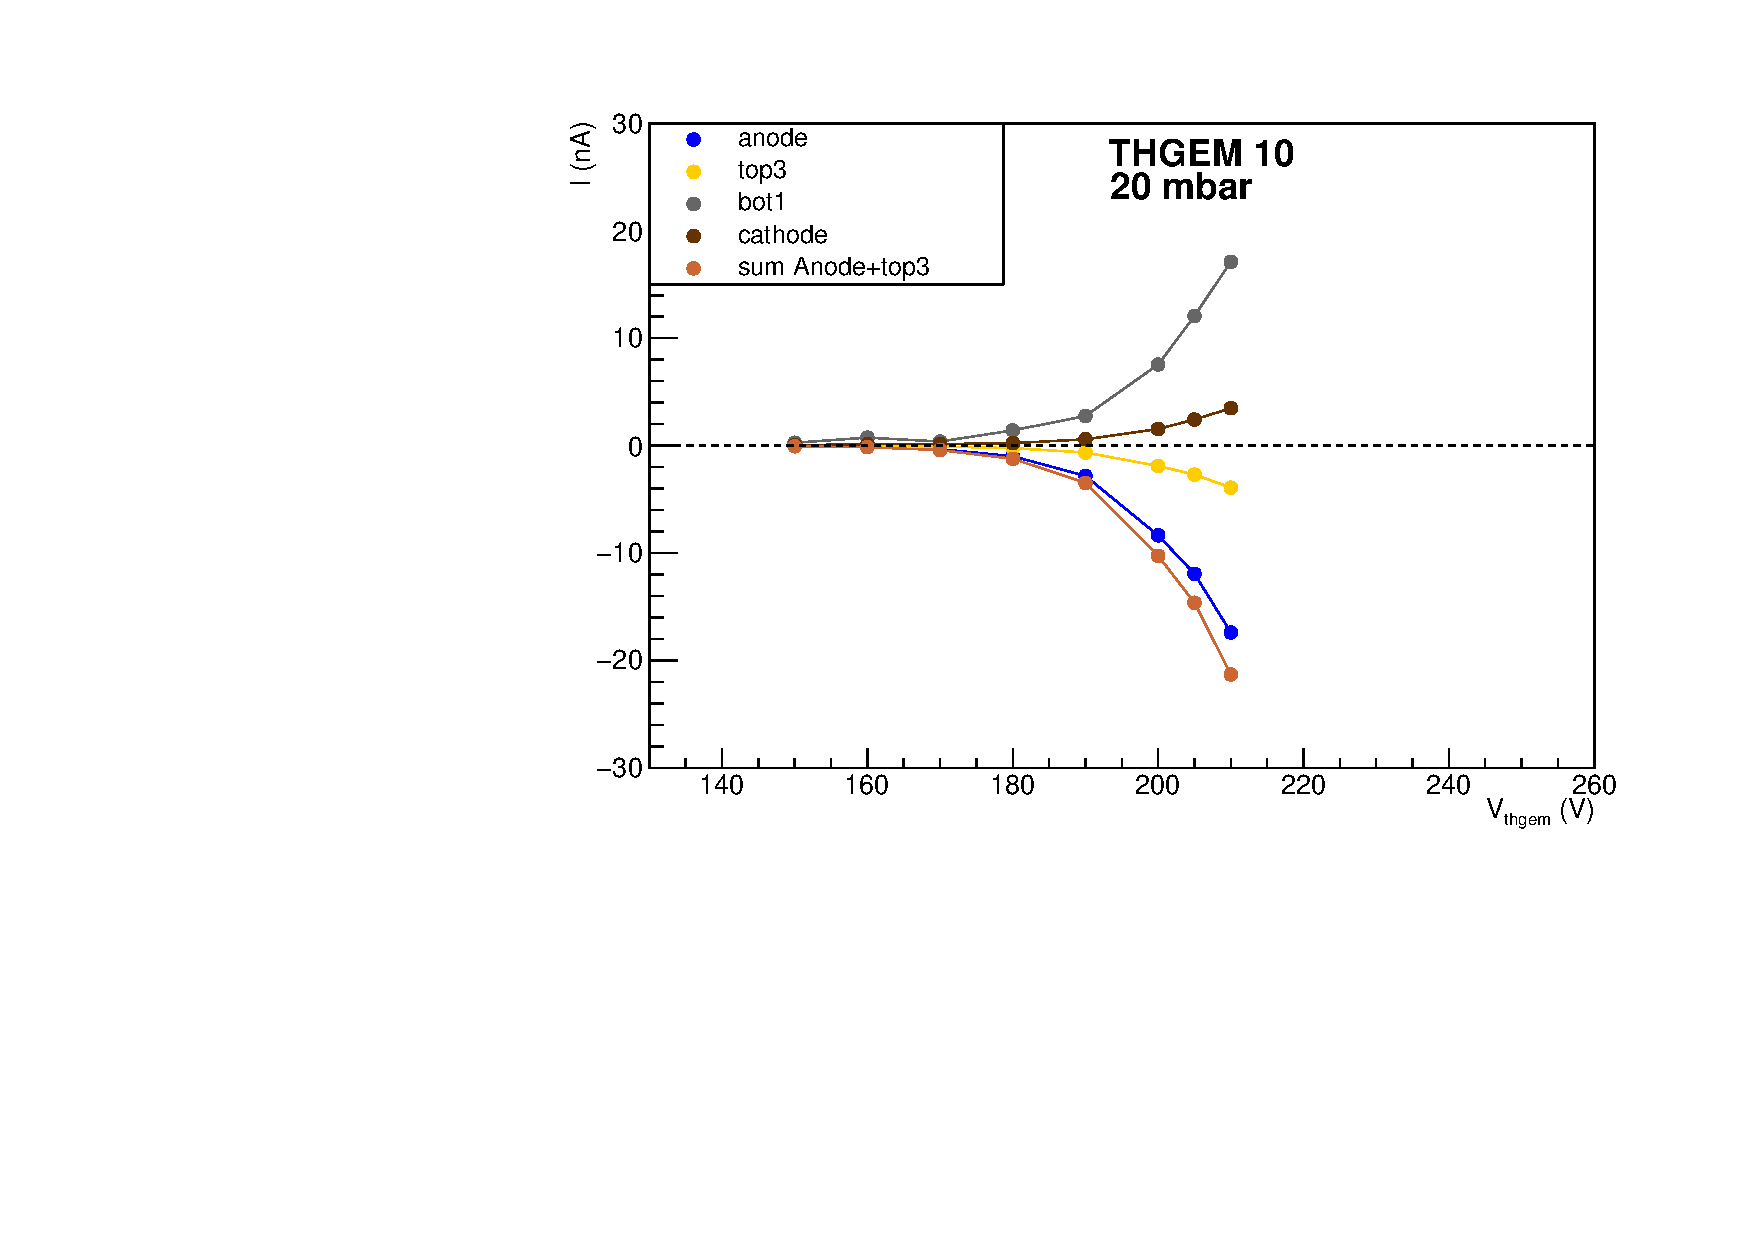
\includegraphics[width=0.96\textwidth]{Immagini/thgemScan_THGEM10_20mbar.pdf}}
	\subfigure[]{ 	\label{fig:thgem_FULLTHGEM_11mbar} 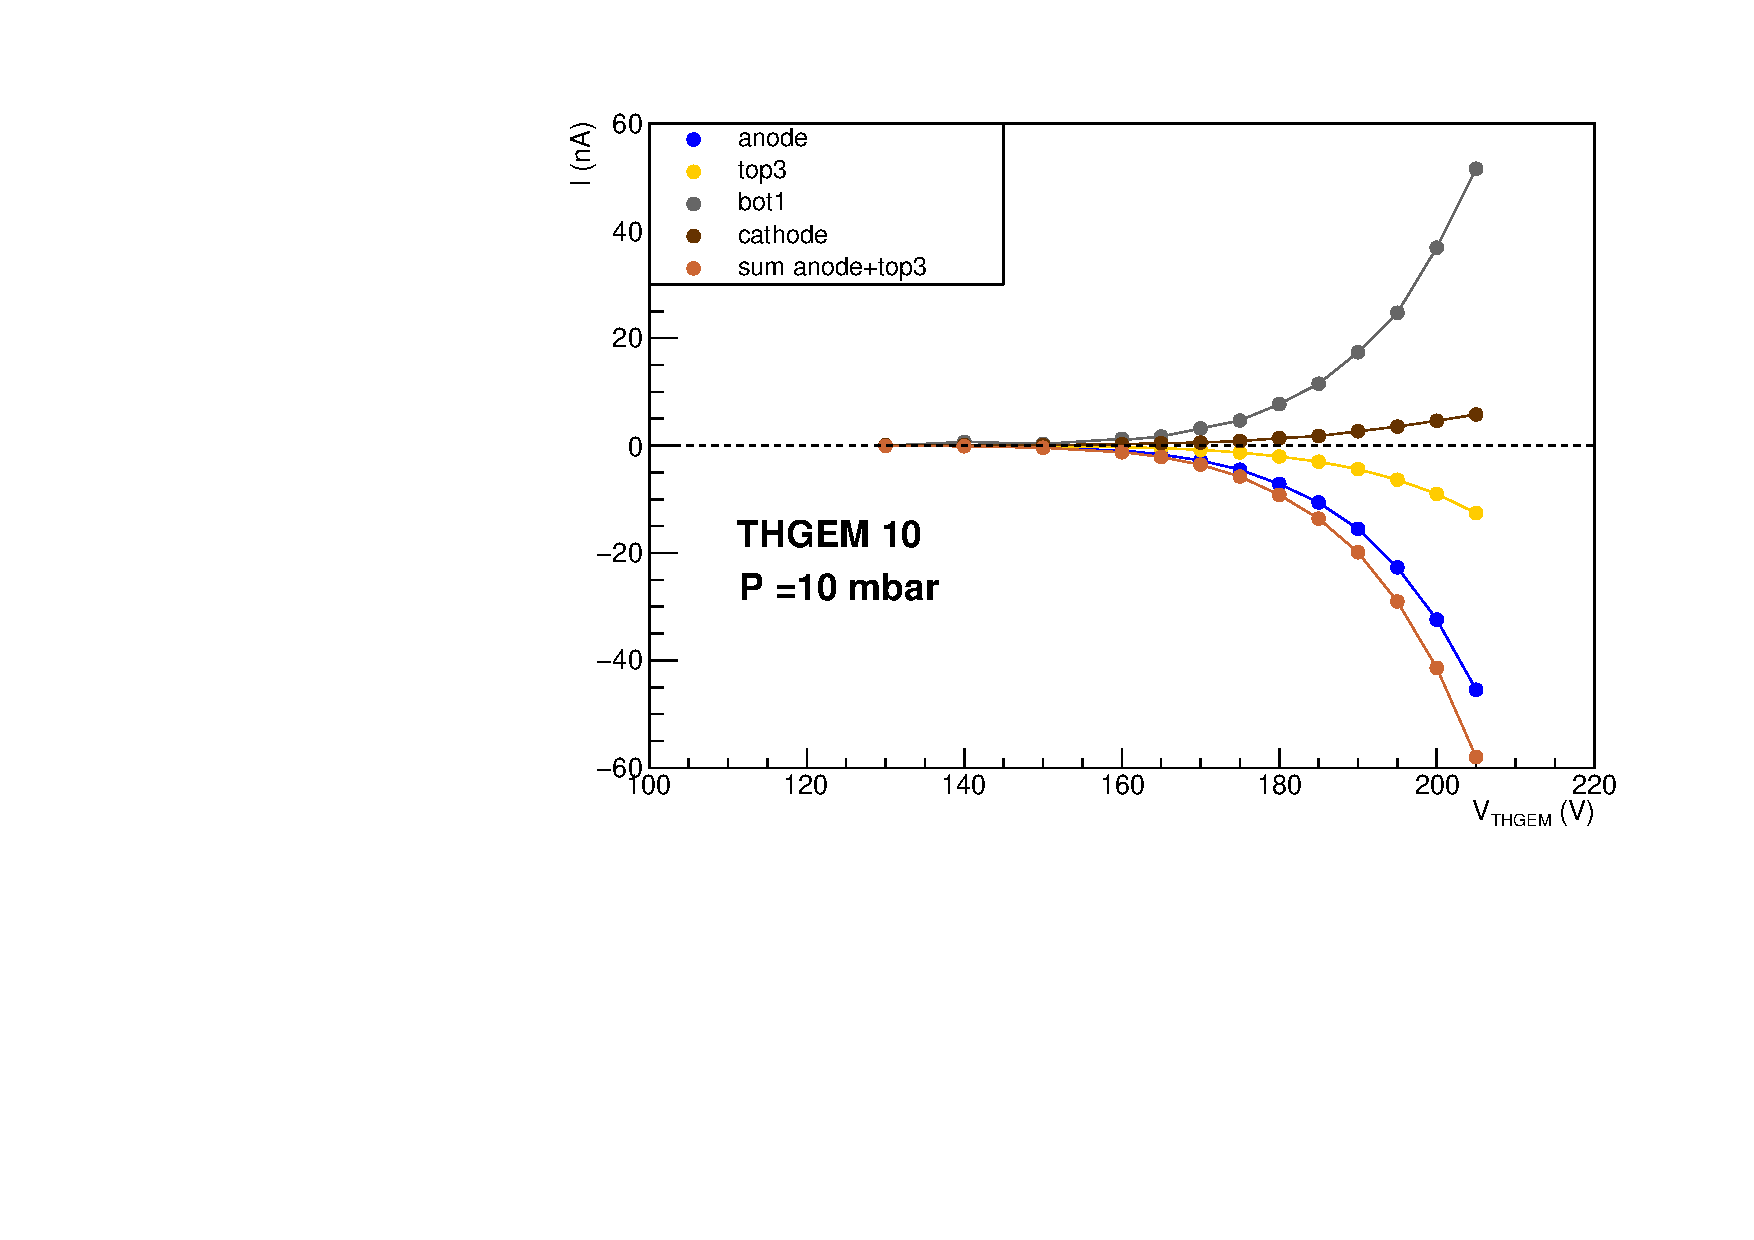
\includegraphics[width=0.96\textwidth]{Immagini/thgemScan_THGEM10_10mbar.pdf}}
	\caption{Currents measured during the scan on the voltage \Vthgem{} across each FULL THGEM: in (a) at 20~mbar, in (b) at 11~mbar.}
	\label{fig:thgem_FULLTHGEM_other_pressure}
\end{figure}

%\textcolor{red}{Aggiungere qui il discorso sul fattore di moltiplicazione?}

From these measurements, the multiplication factors were evaluated as a function of \Vthgem{} and pressure.
The results of the calculations are shown in Figure~\ref{fig:multiplication_factor_FULL}: in the three cases the growth of the electron number in the avalanche follows an exponential behaviour.\\

\begin{figure}[!t]
	\centering
	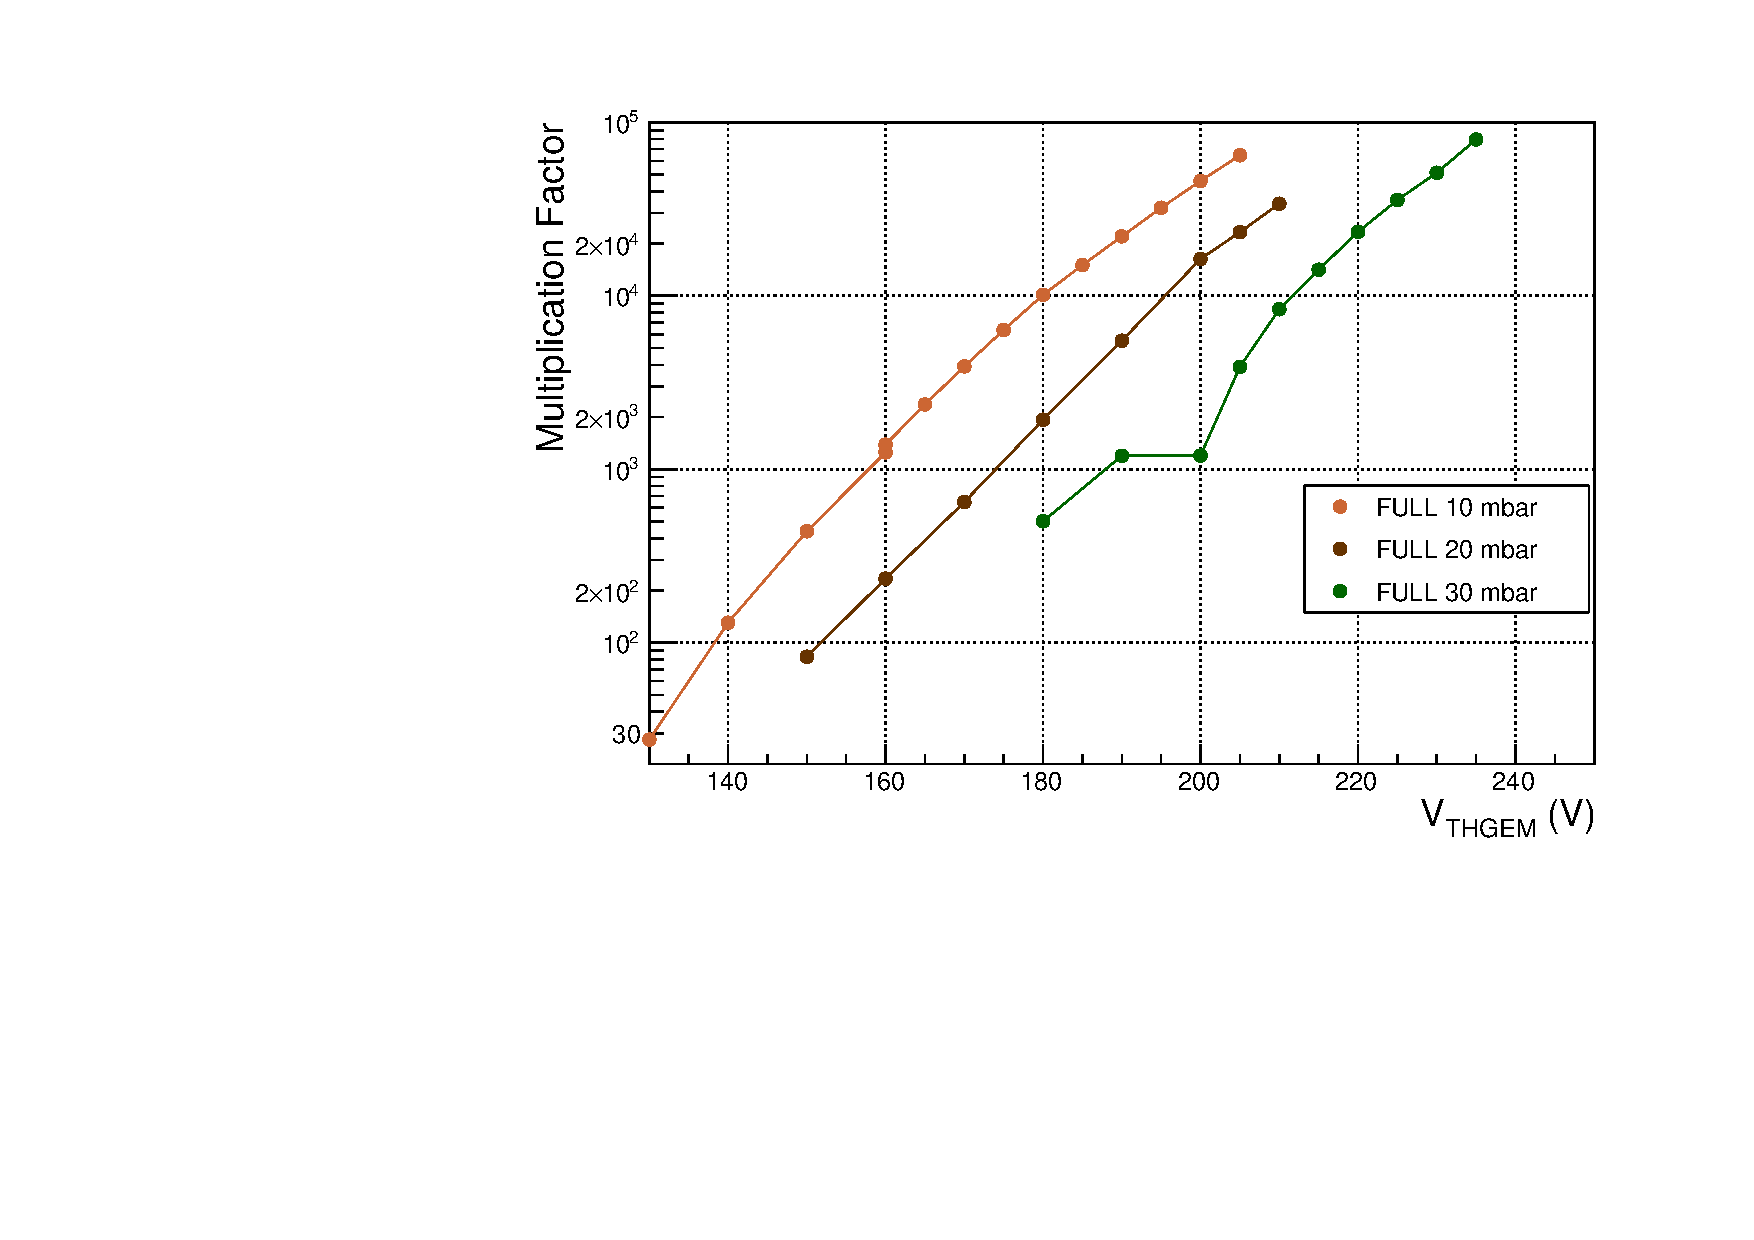
\includegraphics[width=\textwidth]{Immagini/MFvsTHGEM_FULL.pdf}
	\caption{The multiplication factors evaluated for the FULL THGEM as a function of \Vthgem{} and pressure.}
	\label{fig:multiplication_factor_FULL}
\end{figure}

On February 20 2020 another test with alpha source was done in the same condition of test with beam. The currents measured during \Vthgem{} scan have the same behavior of previous test. The difference is the maximum anodic achievable current: ~20 nA fixing \Vind{} = 50 V and \Vdrift{} = 400 V and ~40 nA fixing \Vind{} = 70 V and \Vdrift{} = 600 V.

\begin{figure}[htbp]
	\centering
	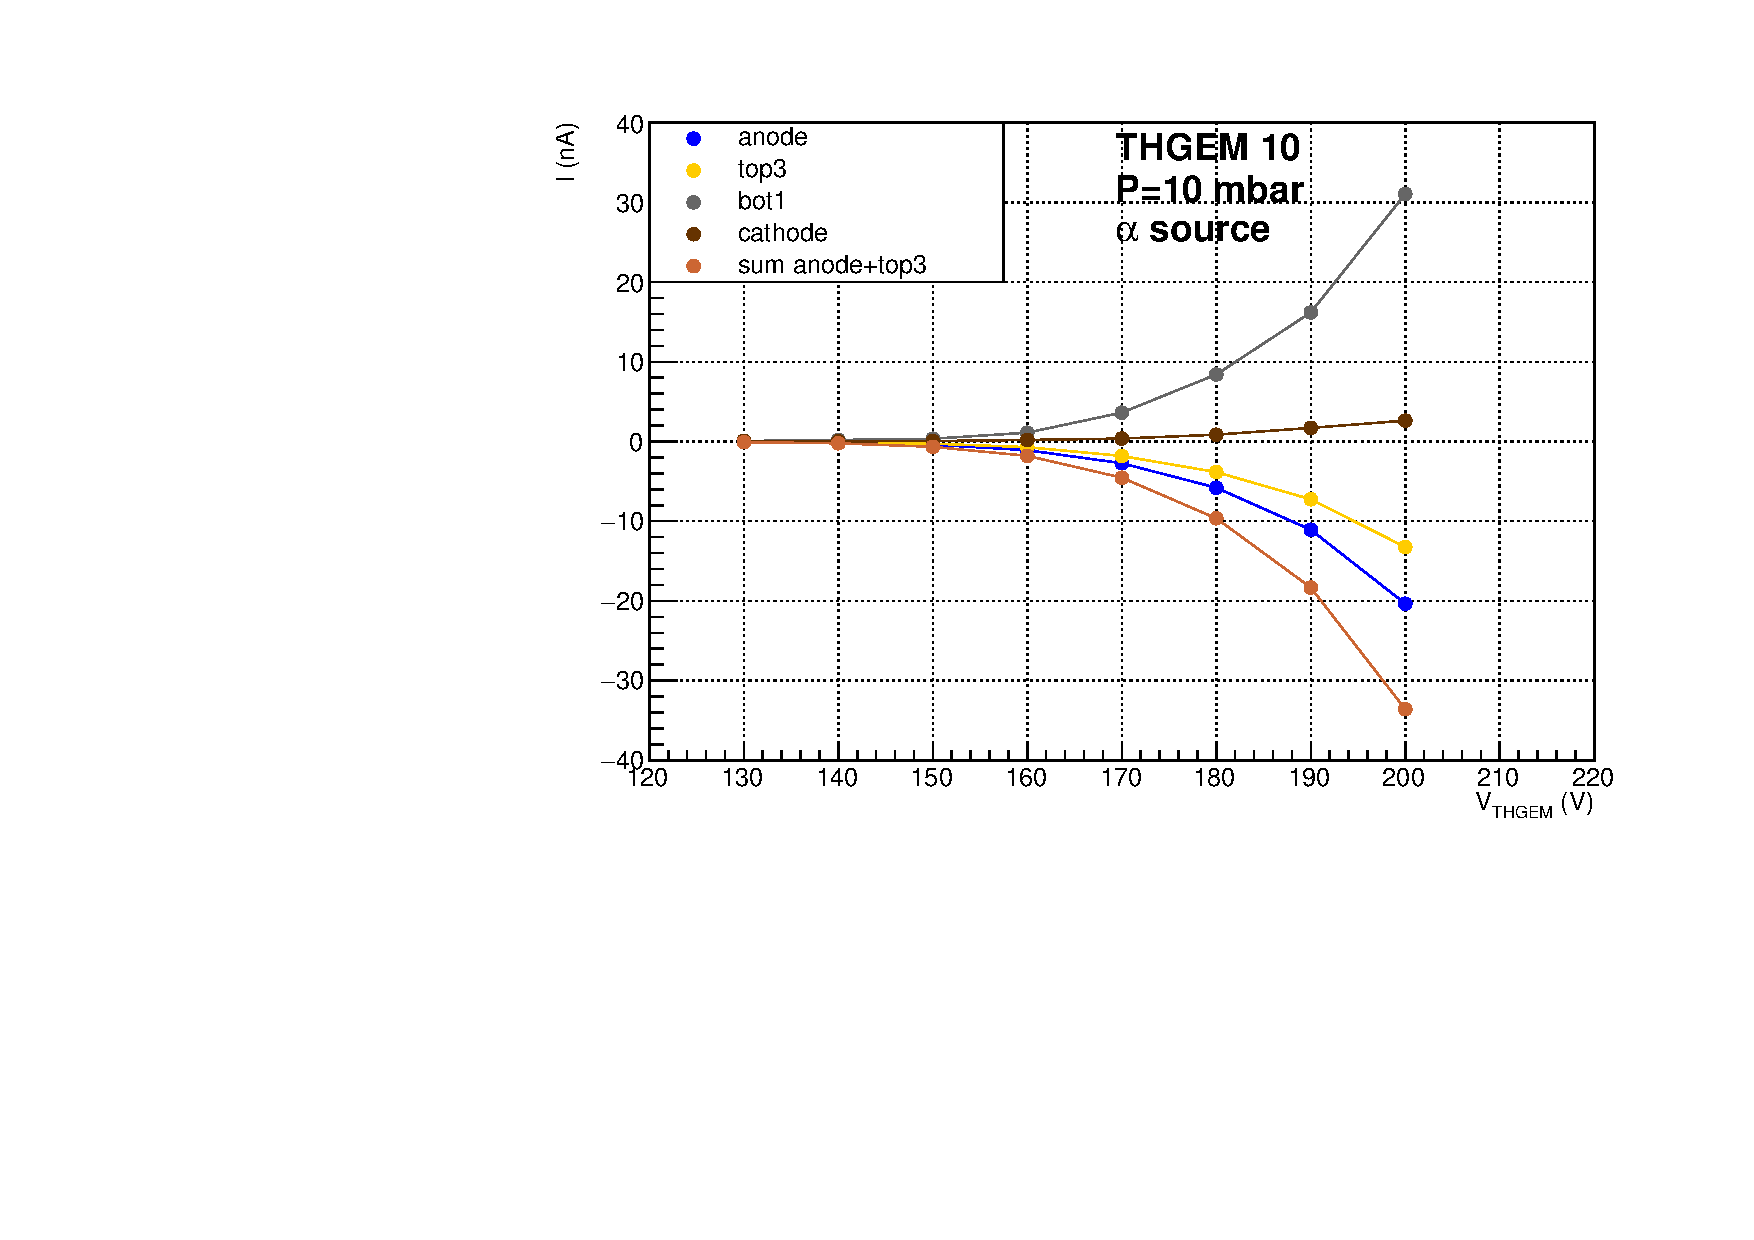
\includegraphics[width=\textwidth]{Immagini/thgemScan_THGEM10_10mbar_bis.pdf}
	\caption{Currents measured during the scan on the voltage \Vthgem{} across the drift region at 10~mbar fixing \Vind{} = 50 V and \Vdrift{} = 400 V.}
	\label{fig:thgem_FULLTHGEM_10mbar_bis}
\end{figure}
%\subsubsection*{Scan on THGEM voltage  at 30 mbar}
%To find the optimal value for the THGEM voltage until discharge, a scan on this parameter has been done. The measured currents obtained for a pressure of 30~mbar and for \Vind~=~120~V and \Vdrift~=~1000~V are shown in Figure~\ref{fig:thgem_FULLTHGEM_30mbar}. \Vthgem~=~180~V is the minimum voltage at which anode current is measurable. At \Vthgem~=~230~V there was discharges, but we do not know if it came from THGEM. The anode current has the typical exponential behaviour.

\clearpage

\subsubsection{Scan on \Vdrift}

To fully characterize the tracker response, a study was conducted varying the potential difference \Vdrift{} across the drift region, while pressure, \Vind{} and \Vthgem{} were kept fixed.
The explored range goes from 0~V (or 100~V in the case with P~=~20~mbar) to the discharge voltage, which depends on the gas pressure: for P~=~30~mbar it was 1600~V, for P~=~20~mbar it was 1200~V, and for P~=~11~mbar it was 800~V.
The increments were of 50~V for P~=~11~mbar, while in the other two cases it was of 100~V.
In Table~\ref{tab:FULLTHGEM_vdrift} the adopted value of pressure, \Vind{} and \Vthgem{} are shown.

\begin{table} [!h]
	\begin{center}
		\renewcommand{\arraystretch}{1.2}
		\begin{tabular} {ccccc}
			P (mbar) & & \Vind{} (V) & & \Vthgem{} (V)\\
			\toprule[0.1em]
			%\hline
			30	& &	120	& &	220 \\
			20	& &	100	& & 205 \\
			11	& & 70	& & 190 \\
			11	& & 70	& & 170 \\
			
			\bottomrule[0.1em]
		\end{tabular}
	\end{center}
	\caption{The values of pressure (P), \Vind{} and \Vthgem{} adopted for the study on \Vdrift.} \label{tab:FULLTHGEM_vdrift}
\end{table}

The result of the scan at 30~mbar is displayed in Figure~\ref{fig:drift_FULLTHGEM_30mbar}. 
All the measured currents are saturated at 100~V.
In order to better understand the THGEM response at low drift voltage, further measurements were done with \Vdrift~=~5~V, 10~V, 20~V, and 30~V.
The result of this measurement, shown in Figure~\textcolor{red}{aggiungere la figura zoomata}, is that currents are saturated already at 5~V.
This means that either the magnitude of the electric field at \Vdrift~=~0~V is much lower than $5/20\; \mbox{(V/cm)}= 250 \; \mbox{(mV/cm)}$ or the value measured by PICO actually is not zero.
\begin{figure}[htbp]
	\centering
	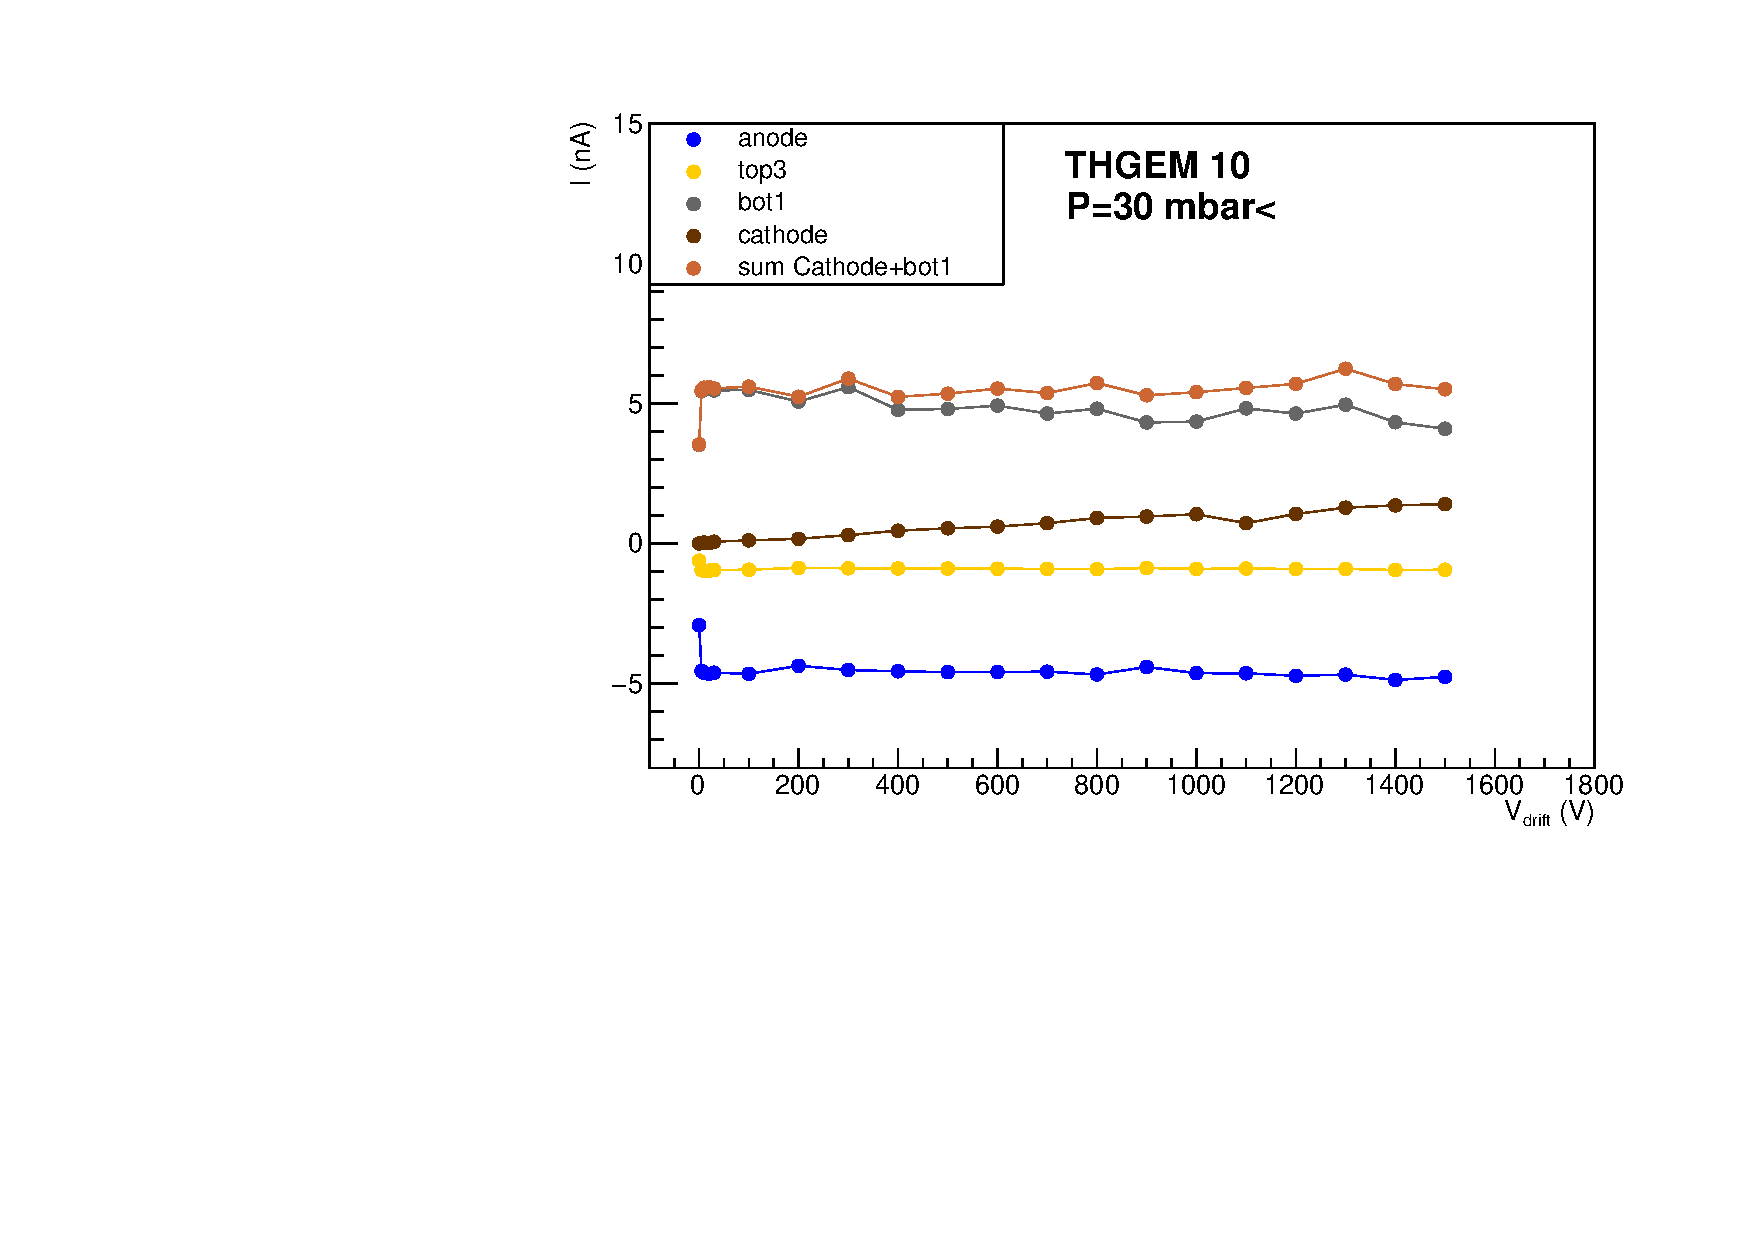
\includegraphics[width=\textwidth]{Immagini/driftScan_THGEM10_30mbar.pdf}
	\caption{Currents measured during the scan on the voltage \Vdrift{} across the drift region at 30~mbar.}
	\label{fig:drift_FULLTHGEM_30mbar}
\end{figure}

In Figure~\ref{fig:drift_FULLTHGEM_30mbar} the orange line represents, in this case, the sum of the cathode and bot1 currents.
This quantity is important to estimate the ion backflow. 
%\textcolor{red}{Aggiungere spiegazione ion backflow}.
%\textcolor{red}{Fare un grafico con l'ion backflow o inserire dei valori di riferimento?}



The results of the tests at 20 and 11~mbar are shown, respectively, in Figure~\ref{fig:drift_FULLTHGEM_20mbar} and~\ref{fig:drift_FULLTHGEM_11mbar}.
Also in these cases the saturation voltage is 100~V.



\begin{figure}[!htb]
	\centering
	\subfigure[]{ \label{fig:drift_FULLTHGEM_20mbar} 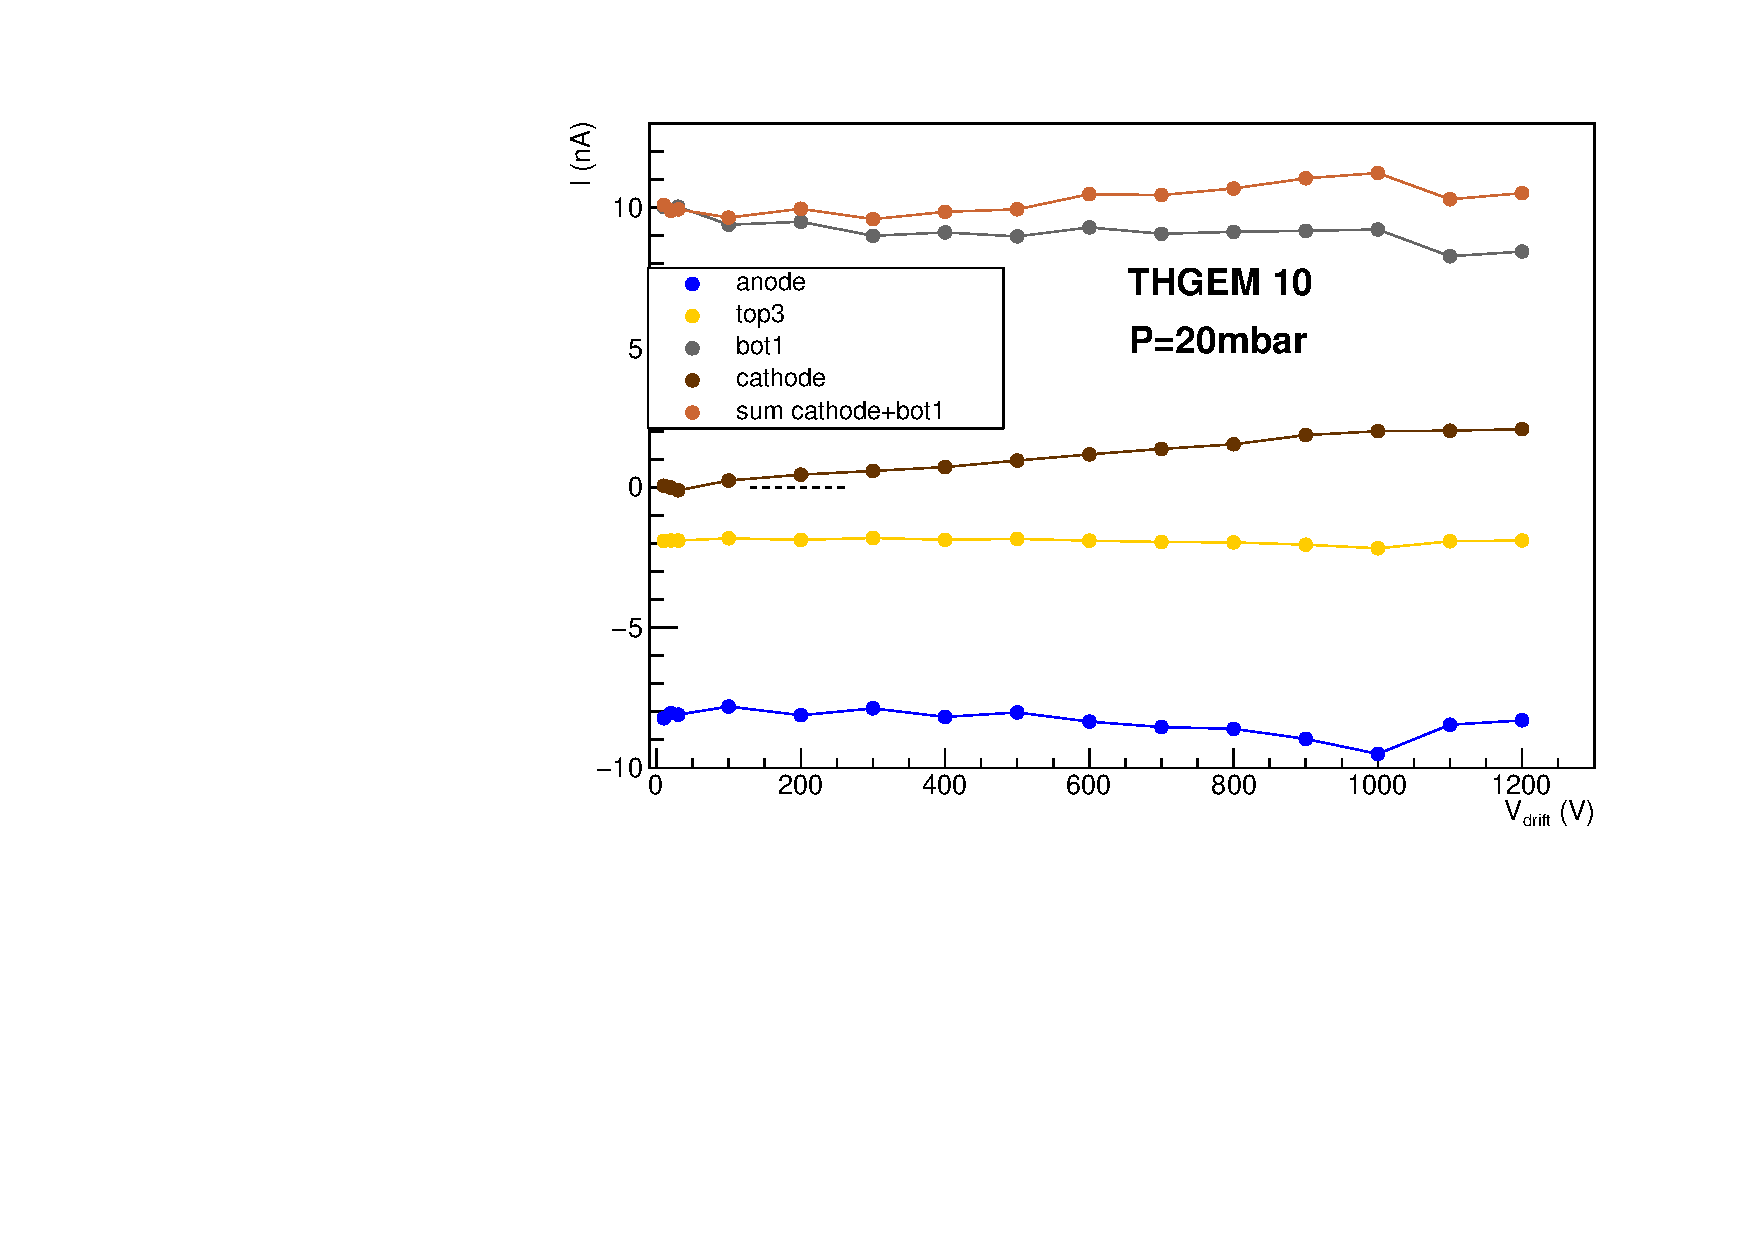
\includegraphics[width=0.96\textwidth]{Immagini/driftScan_THGEM10_20mbar.pdf}}
	\subfigure[]{ 	\label{fig:drift_FULLTHGEM_11mbar} 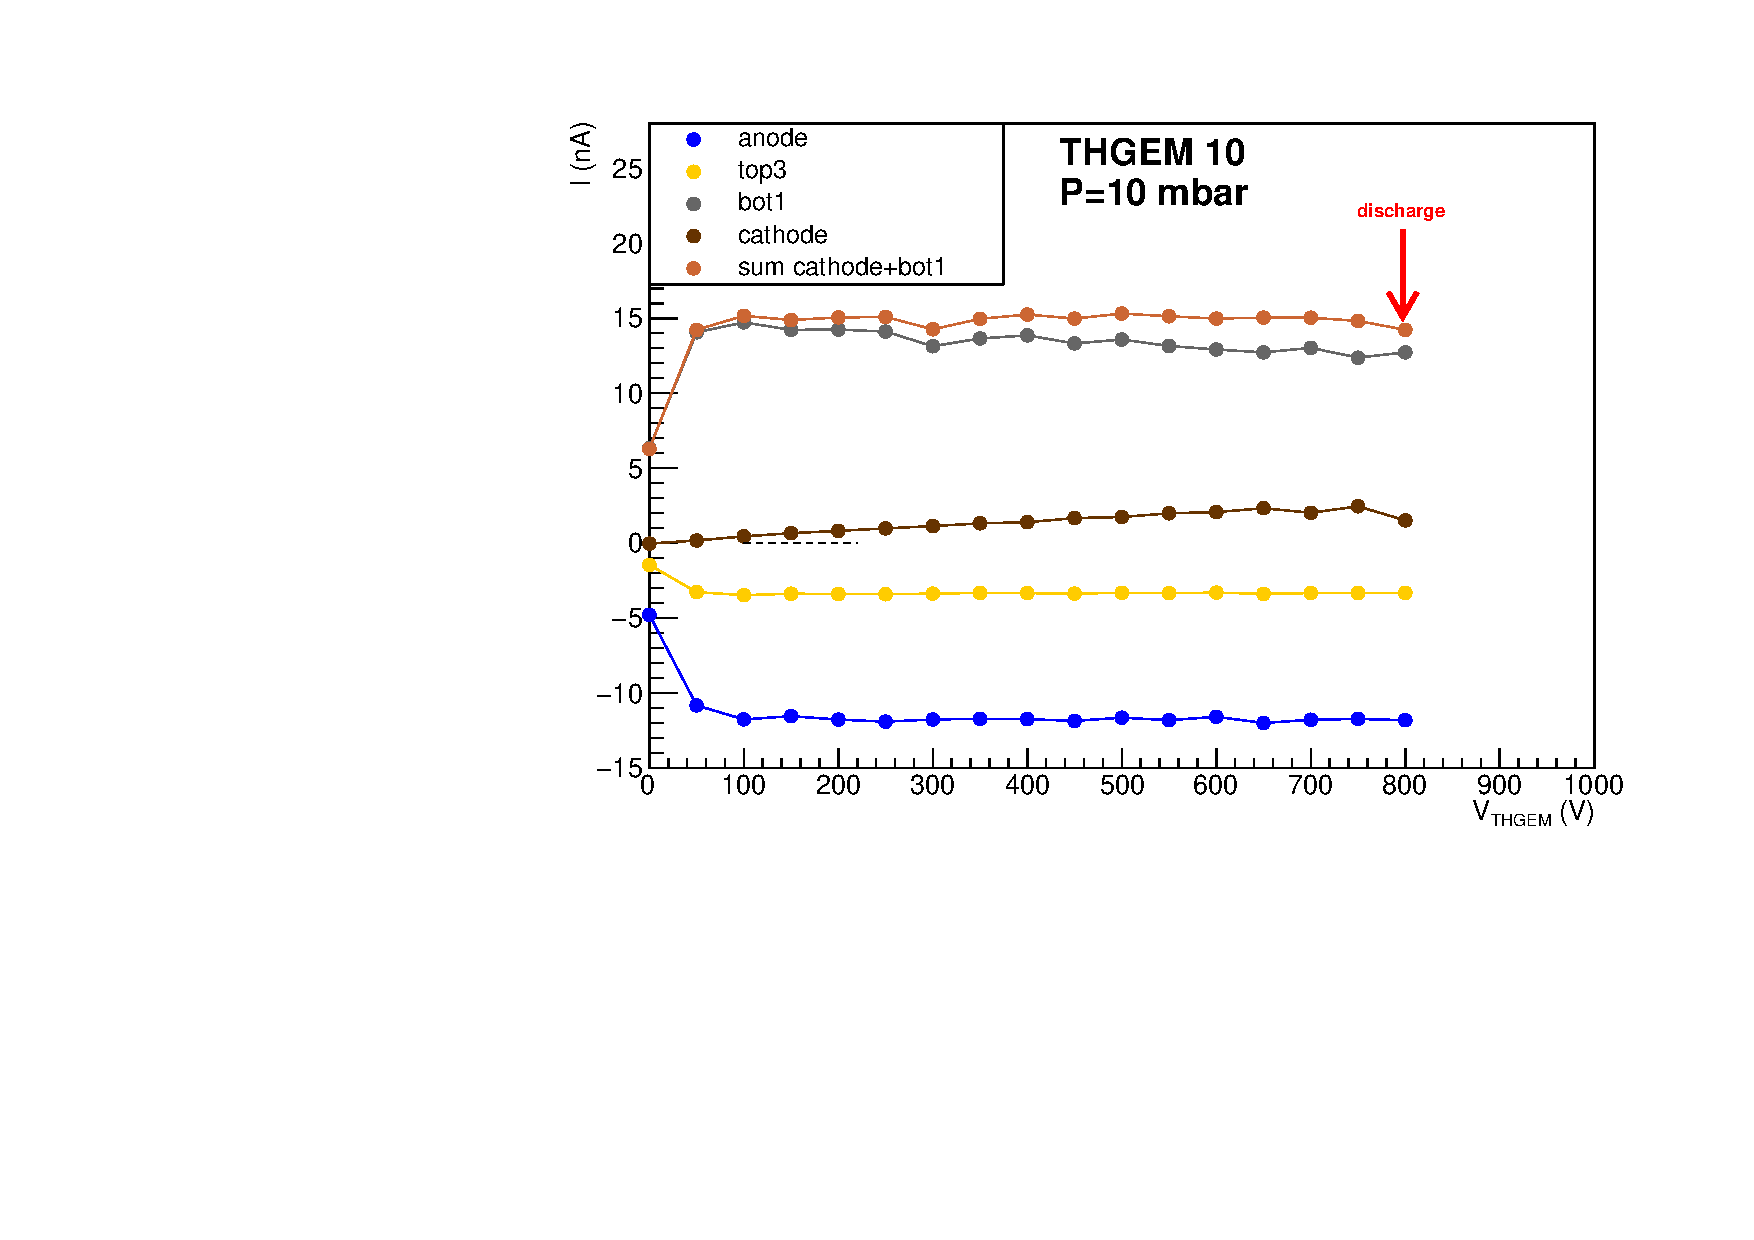
\includegraphics[width=0.96\textwidth]{Immagini/driftScan_THGEM10_10mbar.pdf}}
	\caption{Currents measured during the scan on the voltage \Vdrift{} across the drift region: in (a) at 20~mbar, in (b) at 11~mbar.}
	\label{fig:drift_FULLTHGEM_other_pressure}
\end{figure}



%\textcolor{red}{Aggiungere plot sul backflow}
From these measurements, the ion backflow of the FULL THGEM was evaluated as a function of \Vdrift{} and pressure.
The results of the calculation are shown in Figure~\ref{fig:ion_backflow_FULL}: the ion backflow linearly increases at increasing \Vdrift{} and is almost the same for the three studied pressures.

\begin{figure}[htbp]
	\centering
	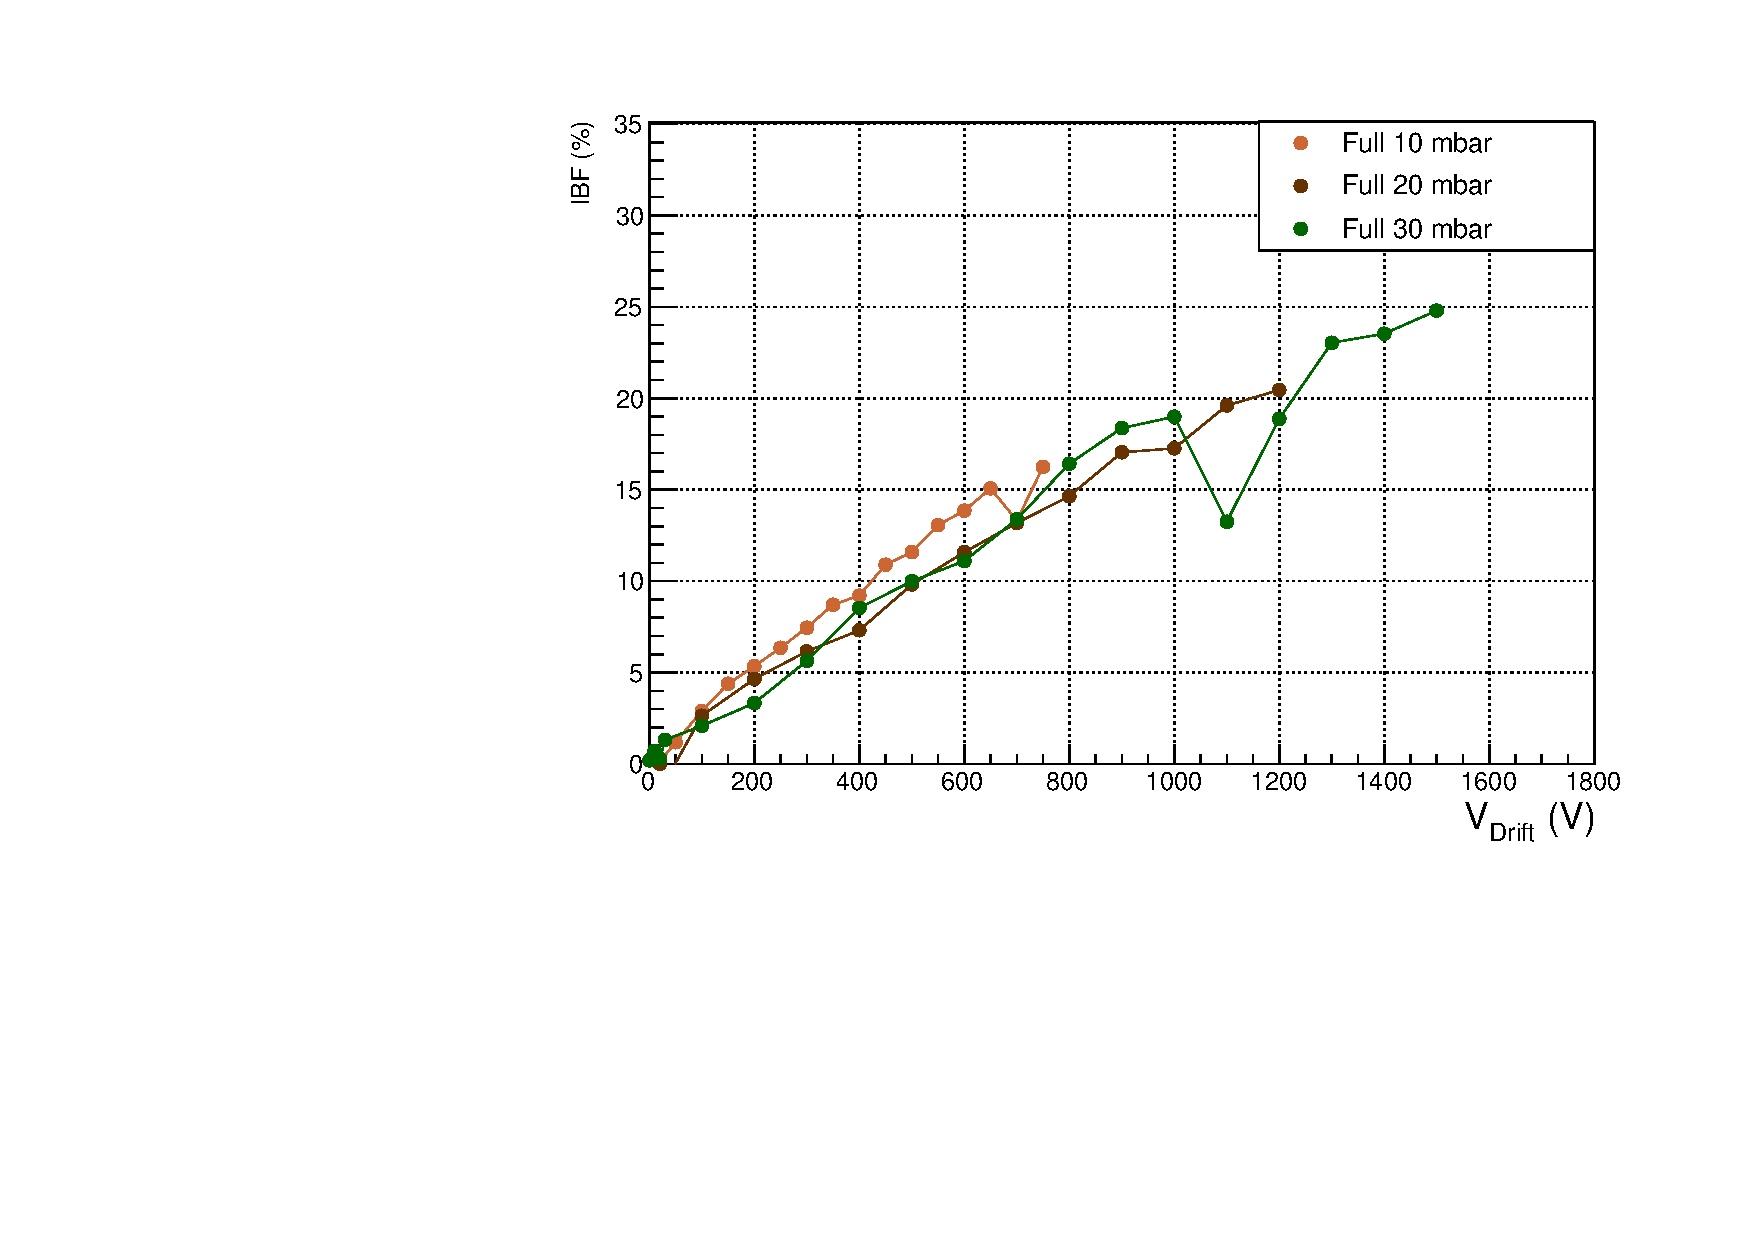
\includegraphics[width=\textwidth]{Immagini/IBFvsDrift_FULLonly.pdf}
	\caption{The ion backflow as a function of \Vdrift{} for the three examined pressures.}
	\label{fig:ion_backflow_FULL}
\end{figure}

On February 20 2020 another test with alpha source was done in the same condition of test with beam. The currents measured during \Vdrift{} scan have the same behavior (almost constant) of previous test. The difference is the current values, a clear example can be anodic current: ~0.5 nA fixing \Vind{} = 50 V and \Vthgem{} = 160 V and ~11 nA fixing \Vind{} = 70 V and \Vthgem{} = 190 V.

\begin{figure}[htbp]
	\centering
	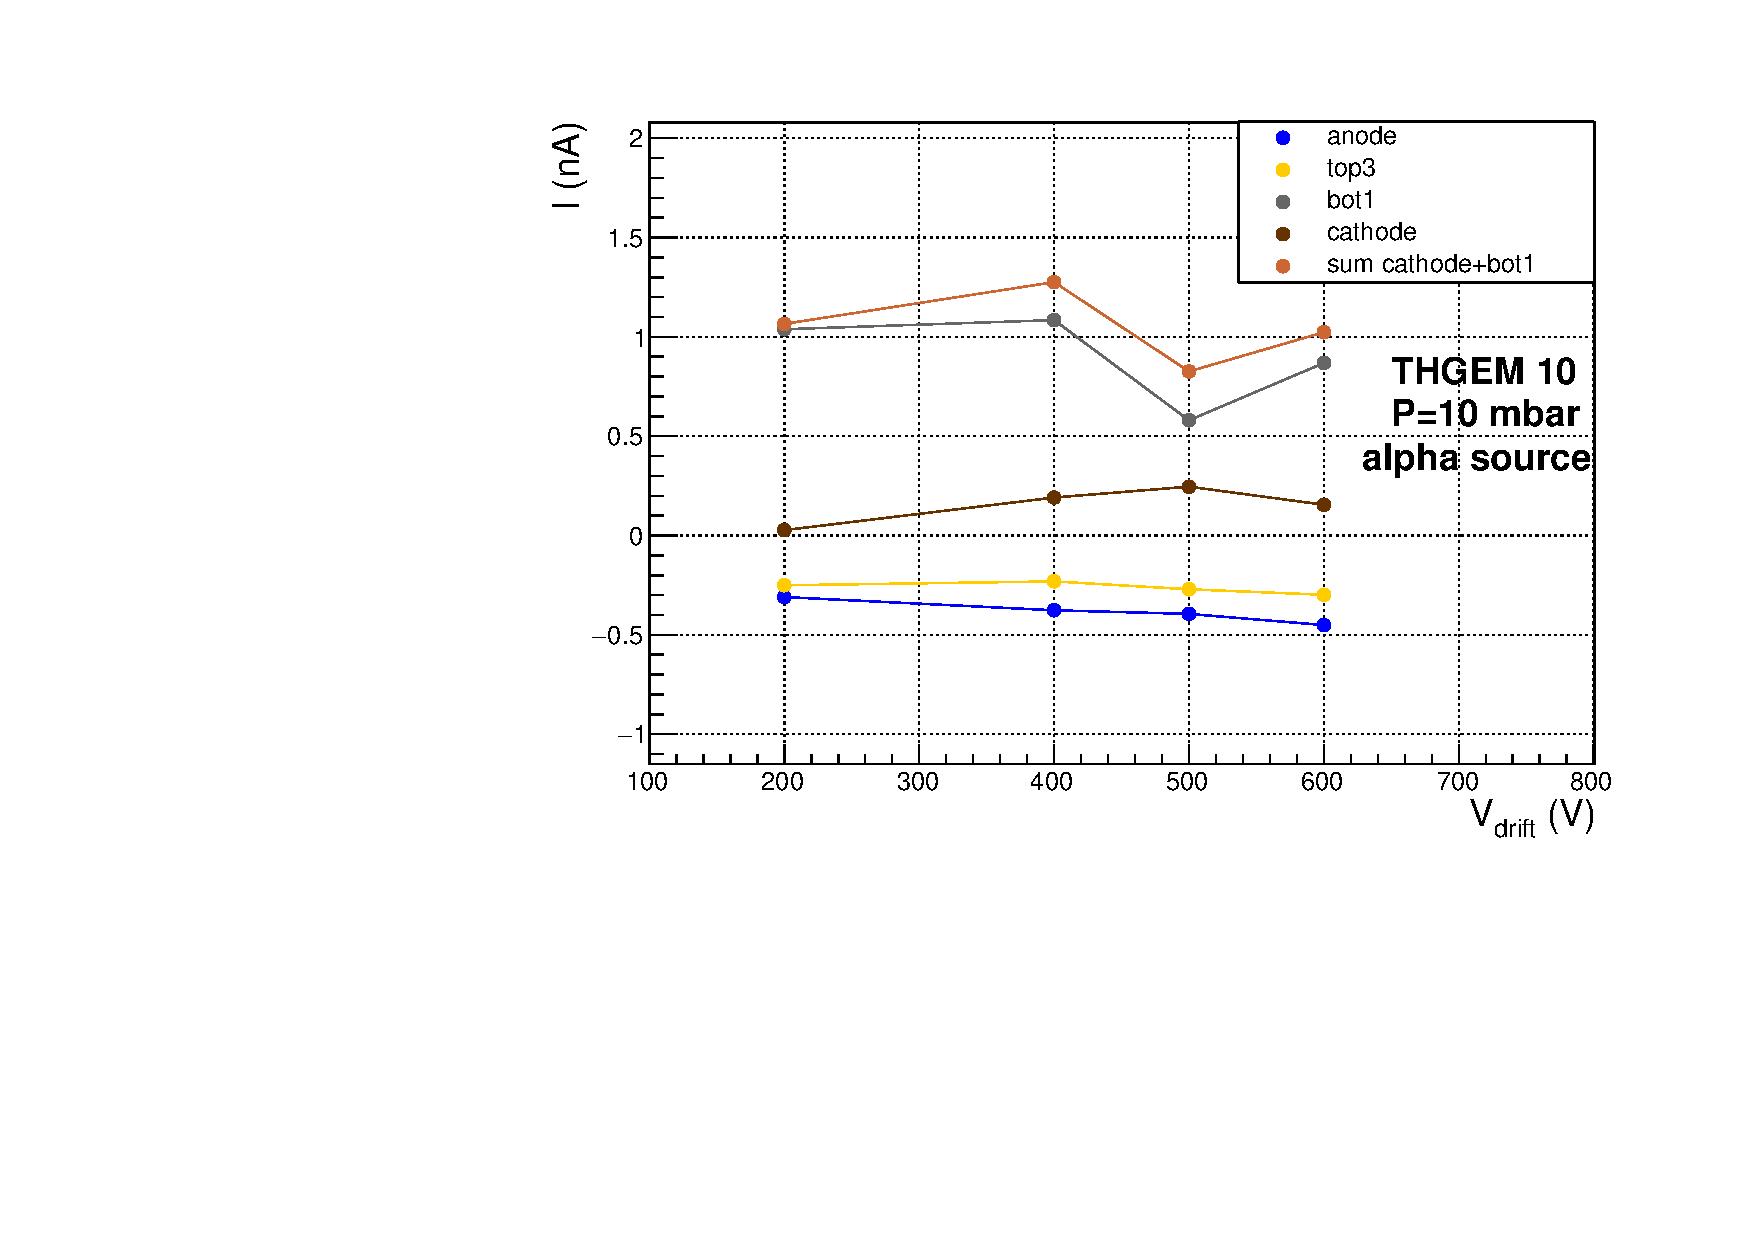
\includegraphics[width=\textwidth]{Immagini/driftScan_THGEM10_alpha_10mbar.pdf}
	\caption{Currents measured during the scan on the voltage \Vdrift{} across the drift region at 10~mbar.}
	\label{fig:driftScan_THGEM10_alpha_10mbar}
\end{figure}

%\subsubsection*{Scan on drift voltage  at 30 mbar}
%To find the optimal value for the drift voltage until discharge, a scan on this parameter has been done. The measured currents obtained for a pressure of 30~mbar and for \Vind~=~120~V and \Vthgem~=~220~V are shown in Figure~\ref{fig:drift_FULLTHGEM_30mbar}. At \Vdrift~=~5~V the anodic current is saturated. This means that the magnitude of the electric field at \Vdrift~=~0~V is much lower than $\frac{5~V}{20~cm}= 250 mV/cm$ or the value measured by PICO is actually not zero. At \Vdrift~=~1200~V ion backflow~(\ibf) is equal to 18.9\%, while at \Vdrift~=~1500~V \ibf~is equal to 24.7\%. Dischages appeared at \Vdrift~=~1600~V.



%\subsubsection*{Scan at 20 mbar}
%The induction, THGEM and drift scan where repeated at 20~mbar and the currents curve show the same behaviour. In \Vind~scan, \Vthgem~=~200~V and \Vdrift~=~1000~V and the plateau was in the range 90$\div$120~V. The optimal value is 100~V. In \Vthgem~scan, \Vind~=~100~V and \Vdrift~=~1000~V and the last measurable signal was at 150~V. At 220~V there were discharges, so the optimal \Vthgem~value is 205~V. During \Vdrift~scan, \Vind~=~100~V and \Vthgem~=~205~V and there were discharges at 1100~V. At \Vdrift~=~700~V, the estimated value of \ibf is 13.2\%, whilst at \Vdrift~=~1000~V  \ibf is 17.3\%.


%\subsubsection*{Scan at 10 mbar}
%The induction, THGEM and drift scan where repeated at 10~mbar and the currents curve show the same behaviour. In \Vind~scan, setting \Vthgem~=~180~V and \Vdrift~=~800~V, discharges appear at 60~V. Setting \Vthgem~=~170~V and \Vdrift~=~800~V, there were discharges mainly in bot1 and cathode currents at 60~V. So the chosen configuration is \Vthgem~=~170~V and \Vdrift~=~600~V. In this way, no discharges were visible.The highest \Vind~value explored was 150~V. Also for this pressure, a plateau was found in the range 60$\div$80~V. The optimal value is 70~V. In \Vthgem~scan, \Vind~=~70~V and \Vdrift~=~600~V and the last measurable signal was at 130~V. At 210~V there were discharges, so the optimal \Vthgem~value is 190~V. During \Vdrift~scan, \Vind~=~70~V and \Vthgem~=~190~V and there were discharges at 800~V. At \Vdrift~=~450~V, the estimated value of \ibf is 10.9\%, whilst at \Vdrift~=~750~V  \ibf is 16.2\%.

\clearpage

\subsection{ROW THGEM}

\subsubsection{Scan on \Vind}

%In the experimental setup employing the ROW THGEM 

%The tracker configuration employing the ROW THGEM was 

%The characterization of the ROW THGEM-based tracker 
%The ROW THGEM-based tracker 

The effects of the variation of the potential difference \Vind{} on the measured currents was studied also for the ROW THGEM-based tracker.
These measurements were done fixing three different pressure (P) and setting suitable values of \Vthgem{} and \Vdrift.
A summary scheme of the adopted configurations is shown in Table~\ref{tab:ROWTHGEM_vind}.
\begin{table} [htbp]
	\begin{center}
		\renewcommand{\arraystretch}{1.2}
		\begin{tabular} {ccccc}
			P (mbar) & & \Vthgem{} (V) & & \Vdrift{} (V)\\
			\toprule[0.1em]
			%\hline
			20	& &	220	& &	800 \\
			20	& & 210	& & 800 \\
			30	& &	240	& &	800 \\
			40	& &	260	& &	700 \\
			
			\bottomrule[0.1em]
		\end{tabular}
	\end{center}
	\caption{The values of pressure (P), \Vthgem{} and \Vdrift{} adopted for the study on \Vind.} \label{tab:ROWTHGEM_vind}
\end{table}
The \Vind{} scans were carried out starting from 0~V and increasing the voltage by 10 or 20~V per run, until the discharge value is reached.
This value is dependent on the gas pressure and on the values set for \Vthgem{} and \Vdrift: for P~=~20~mbar it was 110~V, for P~=~30~mbar it was 110~V, and for P~=~40~mbar it was 180~V.




The result of the two scans at 20~mbar are shown, respectively, in Figure~\ref{fig:induction_ROWTHGEM_20mbar} and~\ref{fig:induction_ROWTHGEM_20mbar_bis}: also with ROW THGEM it is apparent that by raising the value of \Vind{}, the anodic current (blue line) increases, while the top3 current (yellow line) approaches to zero.
%\begin{figure}[htbp]
%	\centering
%	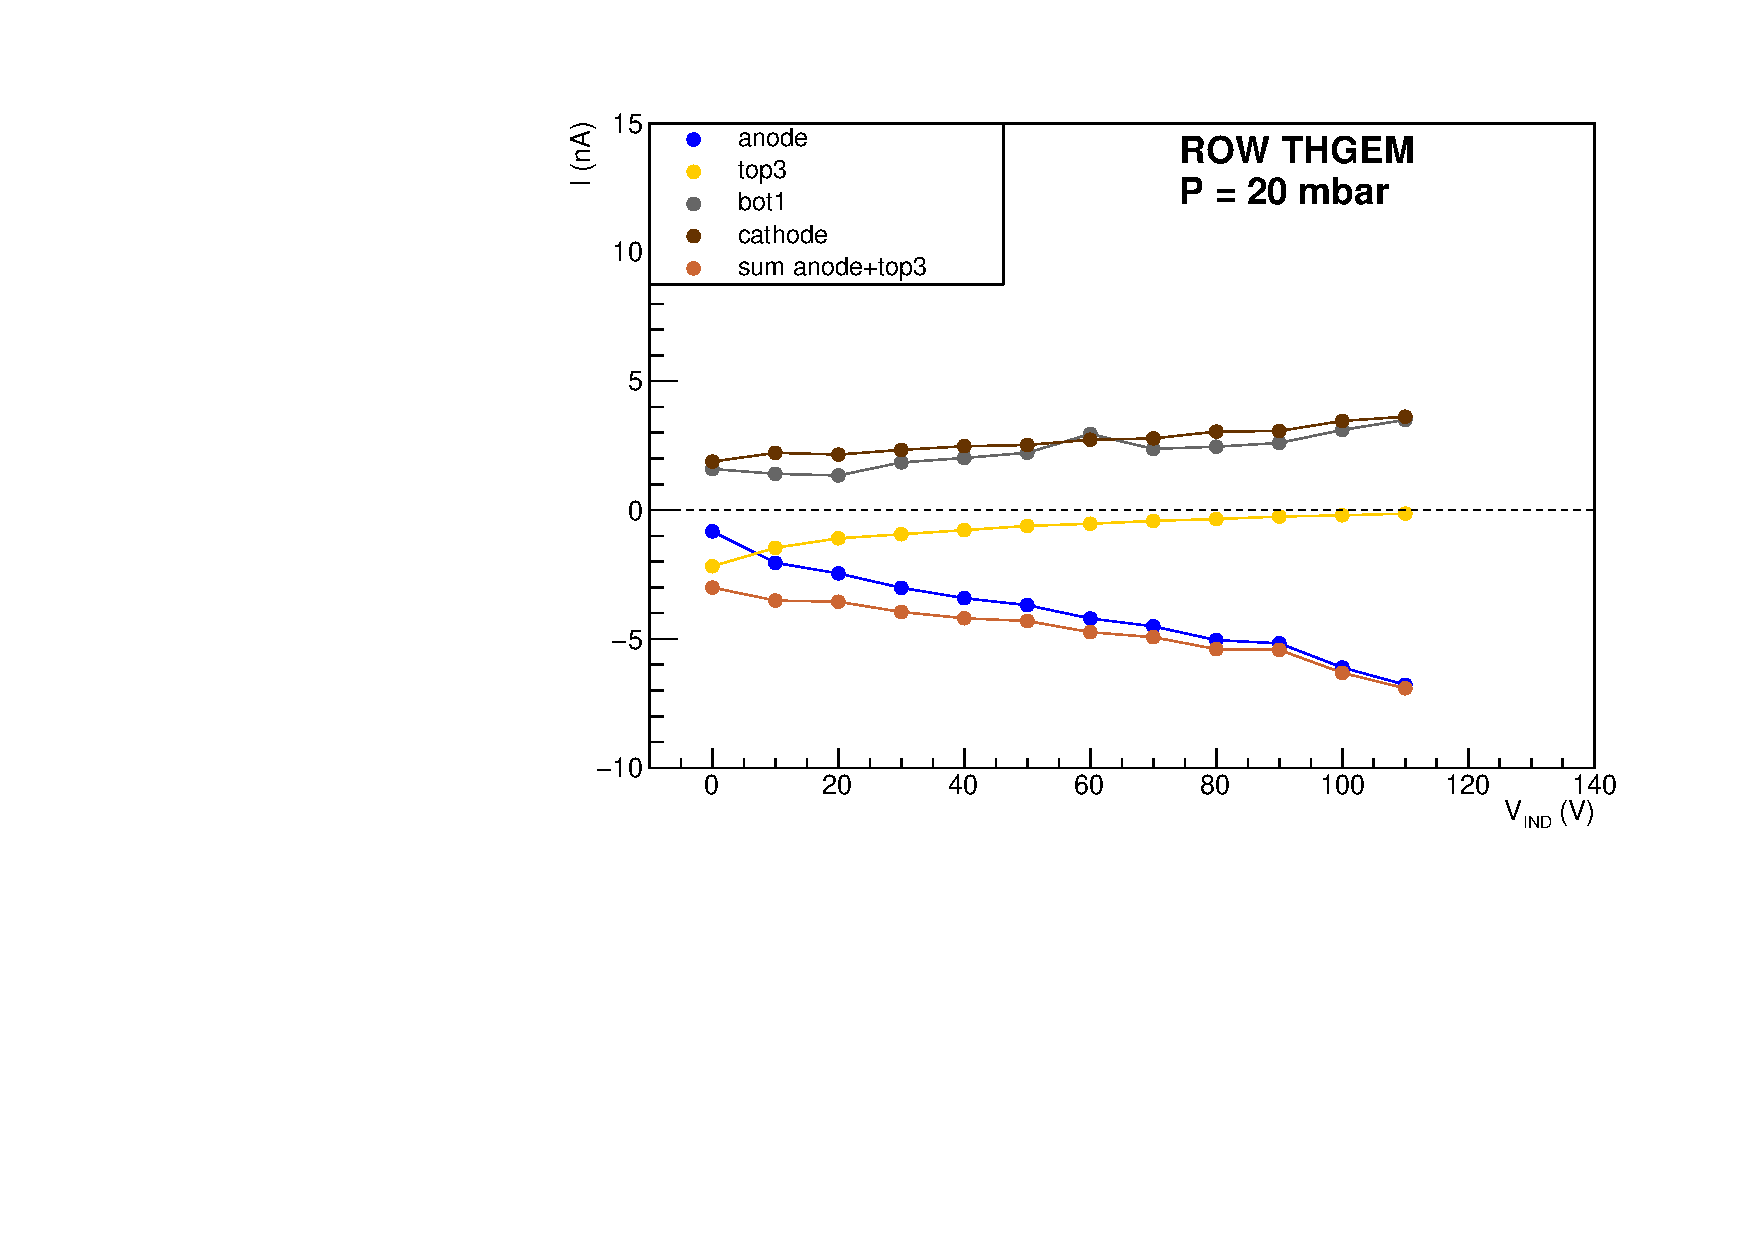
\includegraphics[width=\textwidth]{Immagini/InductionScan_ROW_THGEM_20mbar.pdf}
%	\caption{Currents measured during the scan on the voltage \Vind{} across the induction region at 30~mbar and with \Vthgem{}~=~220~V.}
%	\label{fig:induction_ROWTHGEM_20mbar}
%\end{figure}
\begin{figure}[!htb]
	\centering
	\subfigure[]{ \label{fig:induction_ROWTHGEM_20mbar} 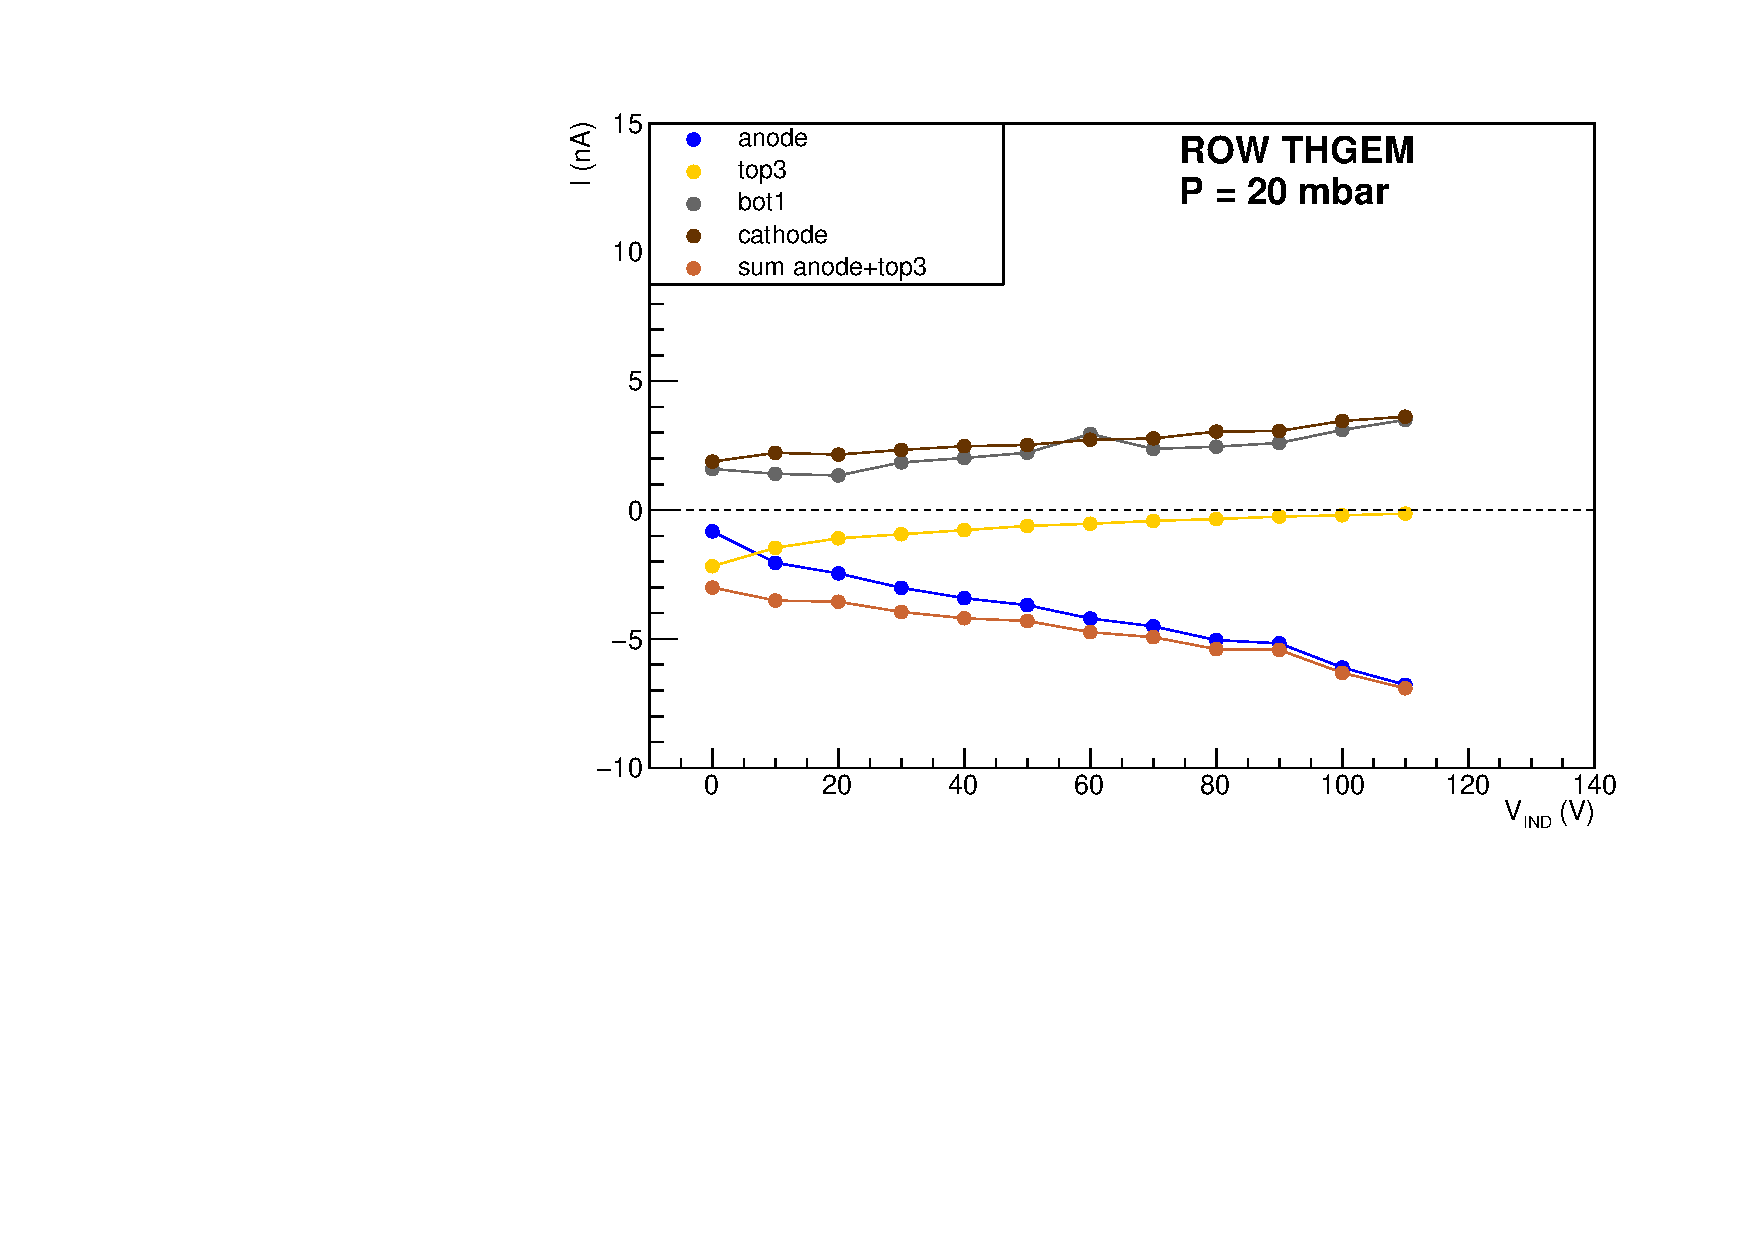
\includegraphics[width=0.96\textwidth]{Immagini/InductionScan_ROW_THGEM_20mbar.pdf}}
	\subfigure[]{ 	\label{fig:induction_ROWTHGEM_20mbar_bis} 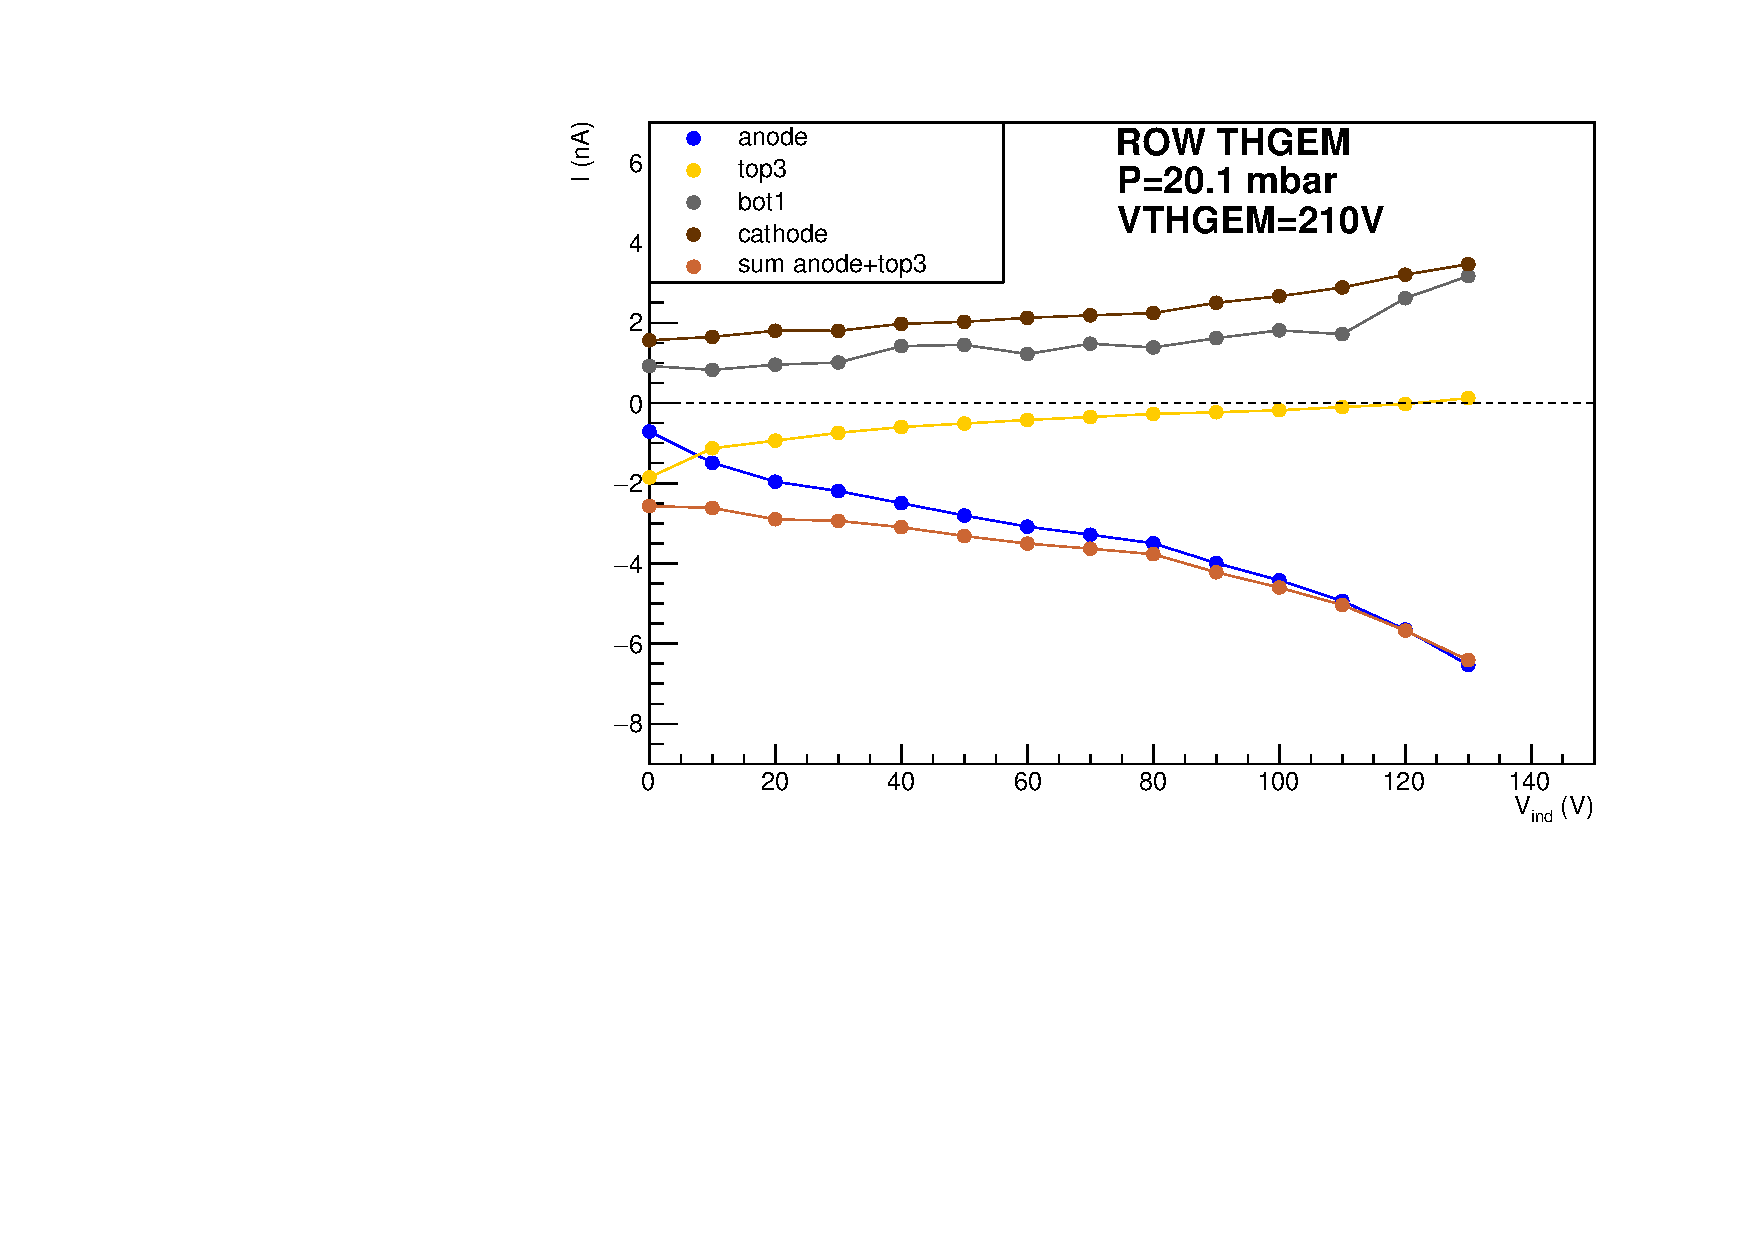
\includegraphics[width=0.96\textwidth]{Immagini/InductionScan_ROW_THGEM_20mbar_bis.pdf}}
	\caption{Currents measured during the scan on the voltage \Vind{} across the induction region at 20~mbar: in (a) \Vthgem{} is at 220~V, in (b) it is at 210~V.}
	\label{fig:induction_ROWTHGEM_20mbar_both}
\end{figure}
Little discharges were observed up to 50~V, while in the range 60$\div$110~V big discharges affected bot1 and top3 currents.
In the case with \Vthgem~=~220~V there is a plateau region from 30 to 70~V, while in that with \Vthgem~=~210~V it is from 30 to 80~V.
\textcolor{red}{giusto?}.
In the former case the optimal value is 50~V, in the latter it is 60~V.



The result of the tests at 30 and 40~mbar are, respectively, shown in Figure~\ref{fig:induction_ROWTHGEM_30mbar} and~\ref{fig:induction_ROWTHGEM_40mbar}.
In the former case the plateau region is clearly visible from 10 to 100~V, so the optimal value is 90~V.
For P~=~40~mbar the plateau region ranges from 20 to 70~V, so the optimal value is 60~V.

%In all the cases the phenomenon of the multiplication 
As for the FULL THGEM, when \Vind{} reaches sufficiently high values, the sum of anode and top3 currents increases, so that the phenomenon of the extension of the multiplication region out of the THGEM holes appears also for the ROW THGEM.

\begin{figure}[!htb]
	\centering
	\subfigure[]{ \label{fig:induction_ROWTHGEM_30mbar} 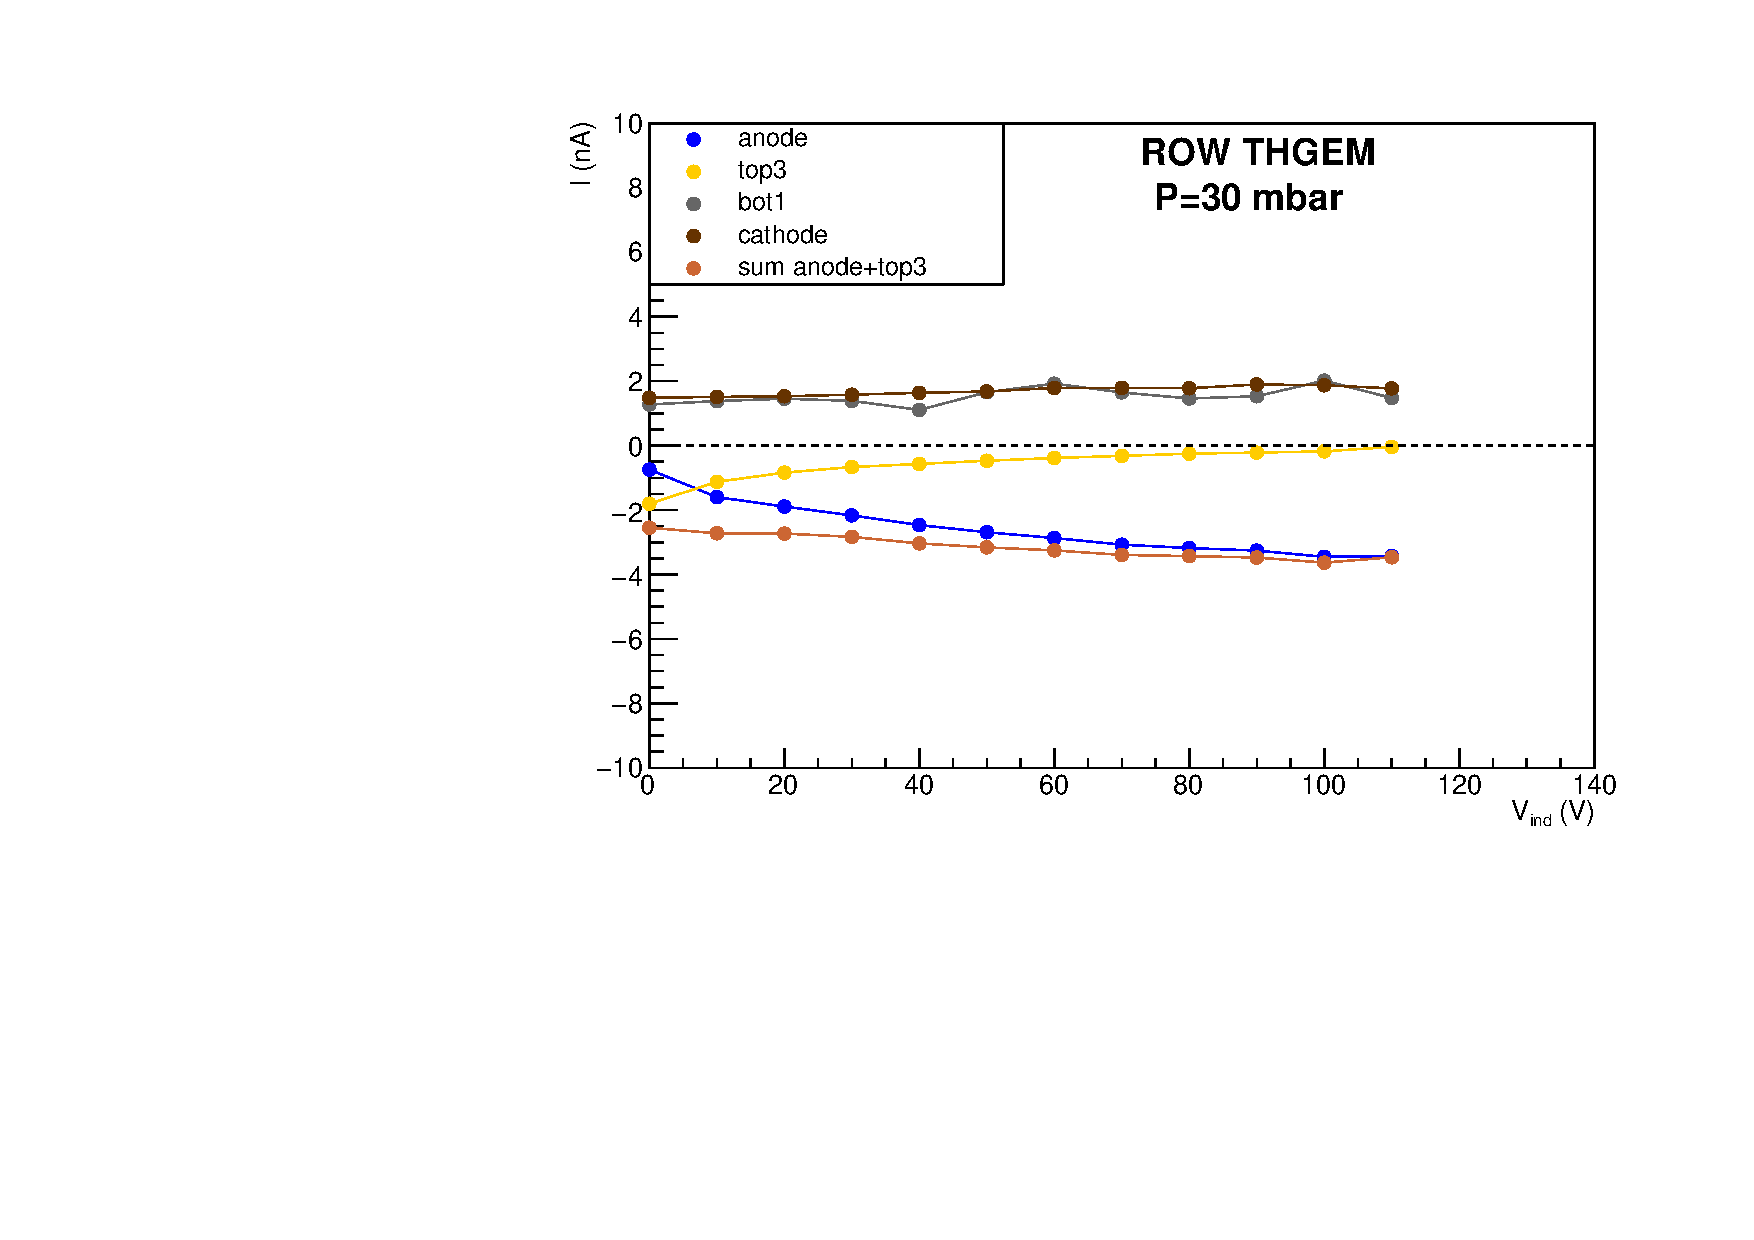
\includegraphics[width=0.96\textwidth]{Immagini/InductionScan_ROW_THGEM_30mbar.pdf}}
	\subfigure[]{ 	\label{fig:induction_ROWTHGEM_40mbar} 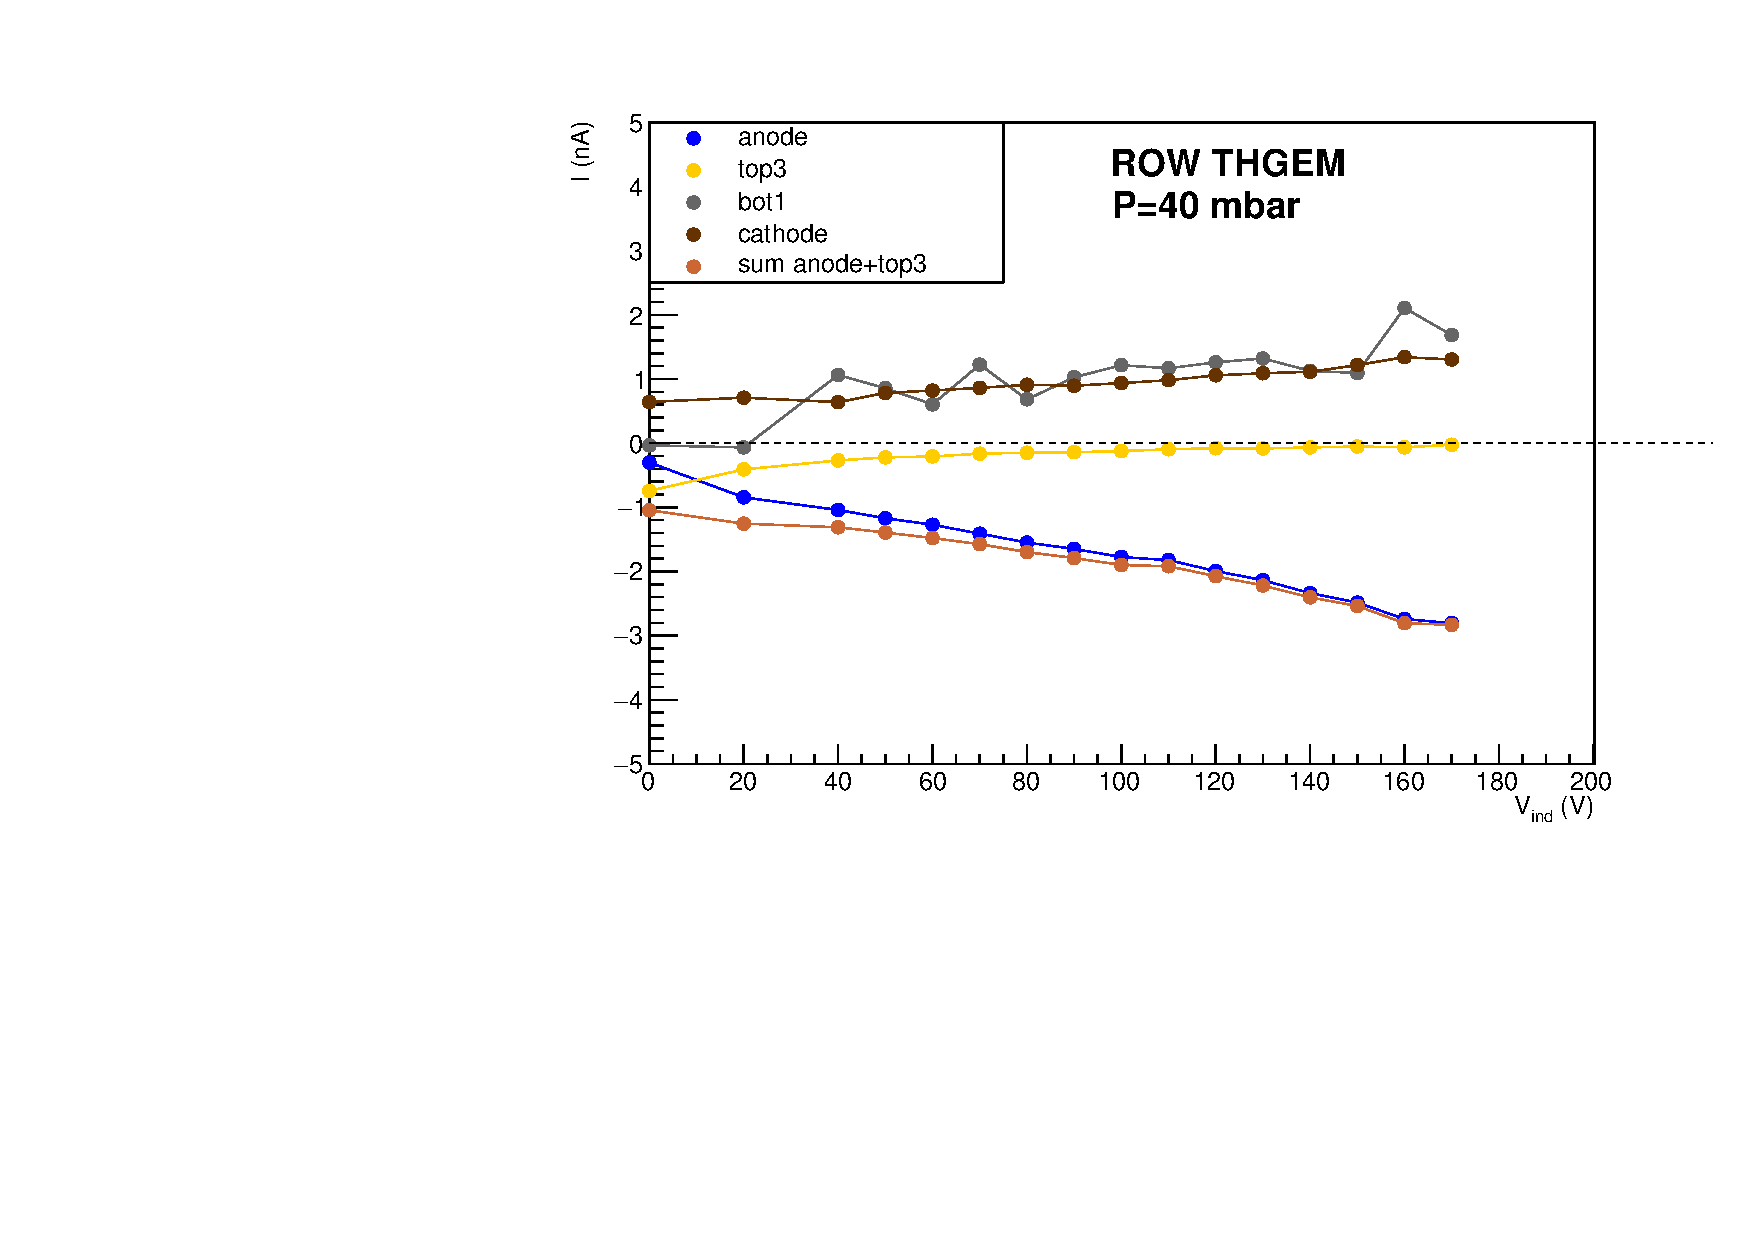
\includegraphics[width=0.96\textwidth]{Immagini/InductionScan_ROW_THGEM_40mbar.pdf}}
	\caption{Currents measured during the scan on the voltage \Vind{} across the induction region: in (a) at 30~mbar, in (b) at 40~mbar.}
	\label{fig:induction_ROWTHGEM_other_pressures}
\end{figure}


%\begin{figure}[htbp]
%	\centering
%	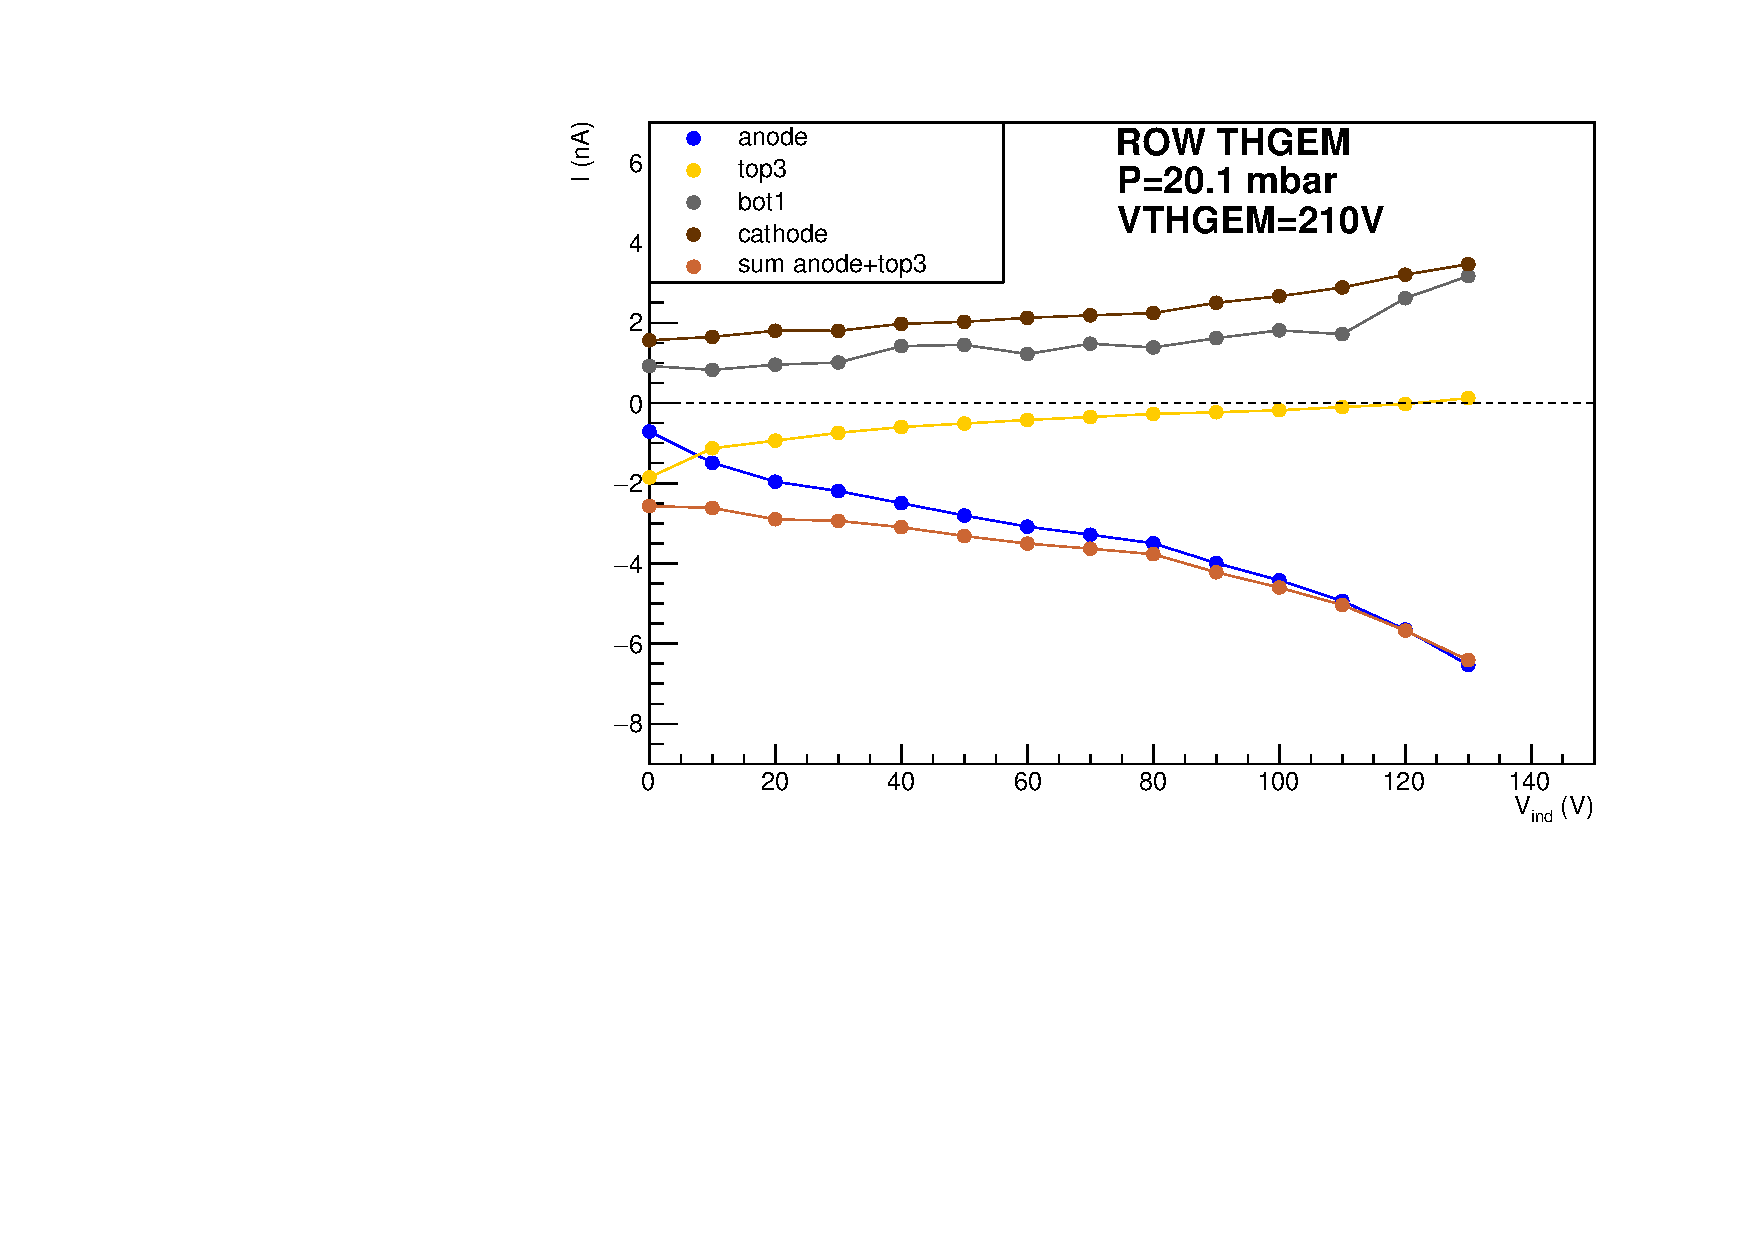
\includegraphics[width=\textwidth]{Immagini/InductionScan_ROW_THGEM_20mbar_bis.pdf}
%	\caption{Currents measured during the scan on the voltage \Vind{} across the induction region at 20~mbar and with \Vthgem{}~=~210~V.}
%	\label{fig:induction_ROWTHGEM_20mbar_bis}
%\end{figure}

%\subsubsection*{Scan at 20 mbar}
%The induction and THGEM scan where repeated at 20~mbar for ROW THGEM and the currents curve show the same behaviour as shown in Figure~\ref{fig:induction_ROWTHGEM_20mbar}. In \Vind~scan, \Vthgem~=~220~V and \Vdrift~=~800~V but plateau is absent. Little discharges were visible up to \Vind~50V while big discharges in the range 60-110V affected bot1 and top3 currents. The optimal value is 50V. In \Vthgem~scan, \Vind~=~50~V and \Vdrift~=~800~V and the last measurable signal was at 180~V. At 225~V there were big discharges, so the optimal \Vthgem~value is 210~V. We do not know if this value is the right one because no drift scan was made. 


\clearpage

\subsubsection{Scan on \Vthgem}

In order to study the multiplication factor of the ROW THGEM in different conditions, a series of measurements was conducted varying the voltage \Vthgem, while pressure, \Vind{} and \Vdrift{} were set to fixed values.
The chosen values of pressure, \Vind{} and \Vdrift{} are shown in Table~\ref{tab:ROWTHGEM_vthgem}.
The \Vthgem{} explored range depends on the selected pressure and on \Vind{} and \Vdrift: for the sake of simplicity these ranges are summarized in Table~\ref{tab:ROWTHGEM_vthgem}.
The increments were ranging from 5 to 10~V.


\begin{table} [htbp]
	\begin{center}
		\renewcommand{\arraystretch}{1.2}
		\begin{tabular} {ccccccc}
			P (mbar) & & \Vind{} (V) & & \Vdrift{} (V) & & \Vthgem{} range (V)\\
			\toprule[0.1em]
			%\hline
			10	& & 50	& & 200	& & 140$\div$205 \\
			20	& &	50	& &	800 & & 180$\div$225 \\
			22	& & 80	& & 300	& & 120$\div$220 \\
			30	& &	70	& & 800 & & 180$\div$240 \\
			32	& & 70	& &	400	& & 170$\div$245 \\
			42	& & 80	& & 700 & & 220$\div$270 \\

			
			\bottomrule[0.1em]
		\end{tabular}
	\end{center}
	\caption{The values of pressure, \Vind{} and \Vdrift{} adopted for the study on \Vthgem.} \label{tab:ROWTHGEM_vthgem}
\end{table}

%\textcolor{red}{Visto che i grafici sarebbero tanti, sarebbe meglio metterne soltanto due o tre pi\F9 esemplificativi?}

The results of the scans at 10 and 32~mbar are shown, respectively, in Figure~\ref{fig:thgem_ROWTHGEM_10mbar} and~\ref{fig:thgem_ROWTHGEM_30mbar_bis}: the typical exponential growth of the currents is verified also for the ROW THGEM.
 

\begin{figure}[!htb]
	\centering
	\subfigure[]{ \label{fig:thgem_ROWTHGEM_10mbar} 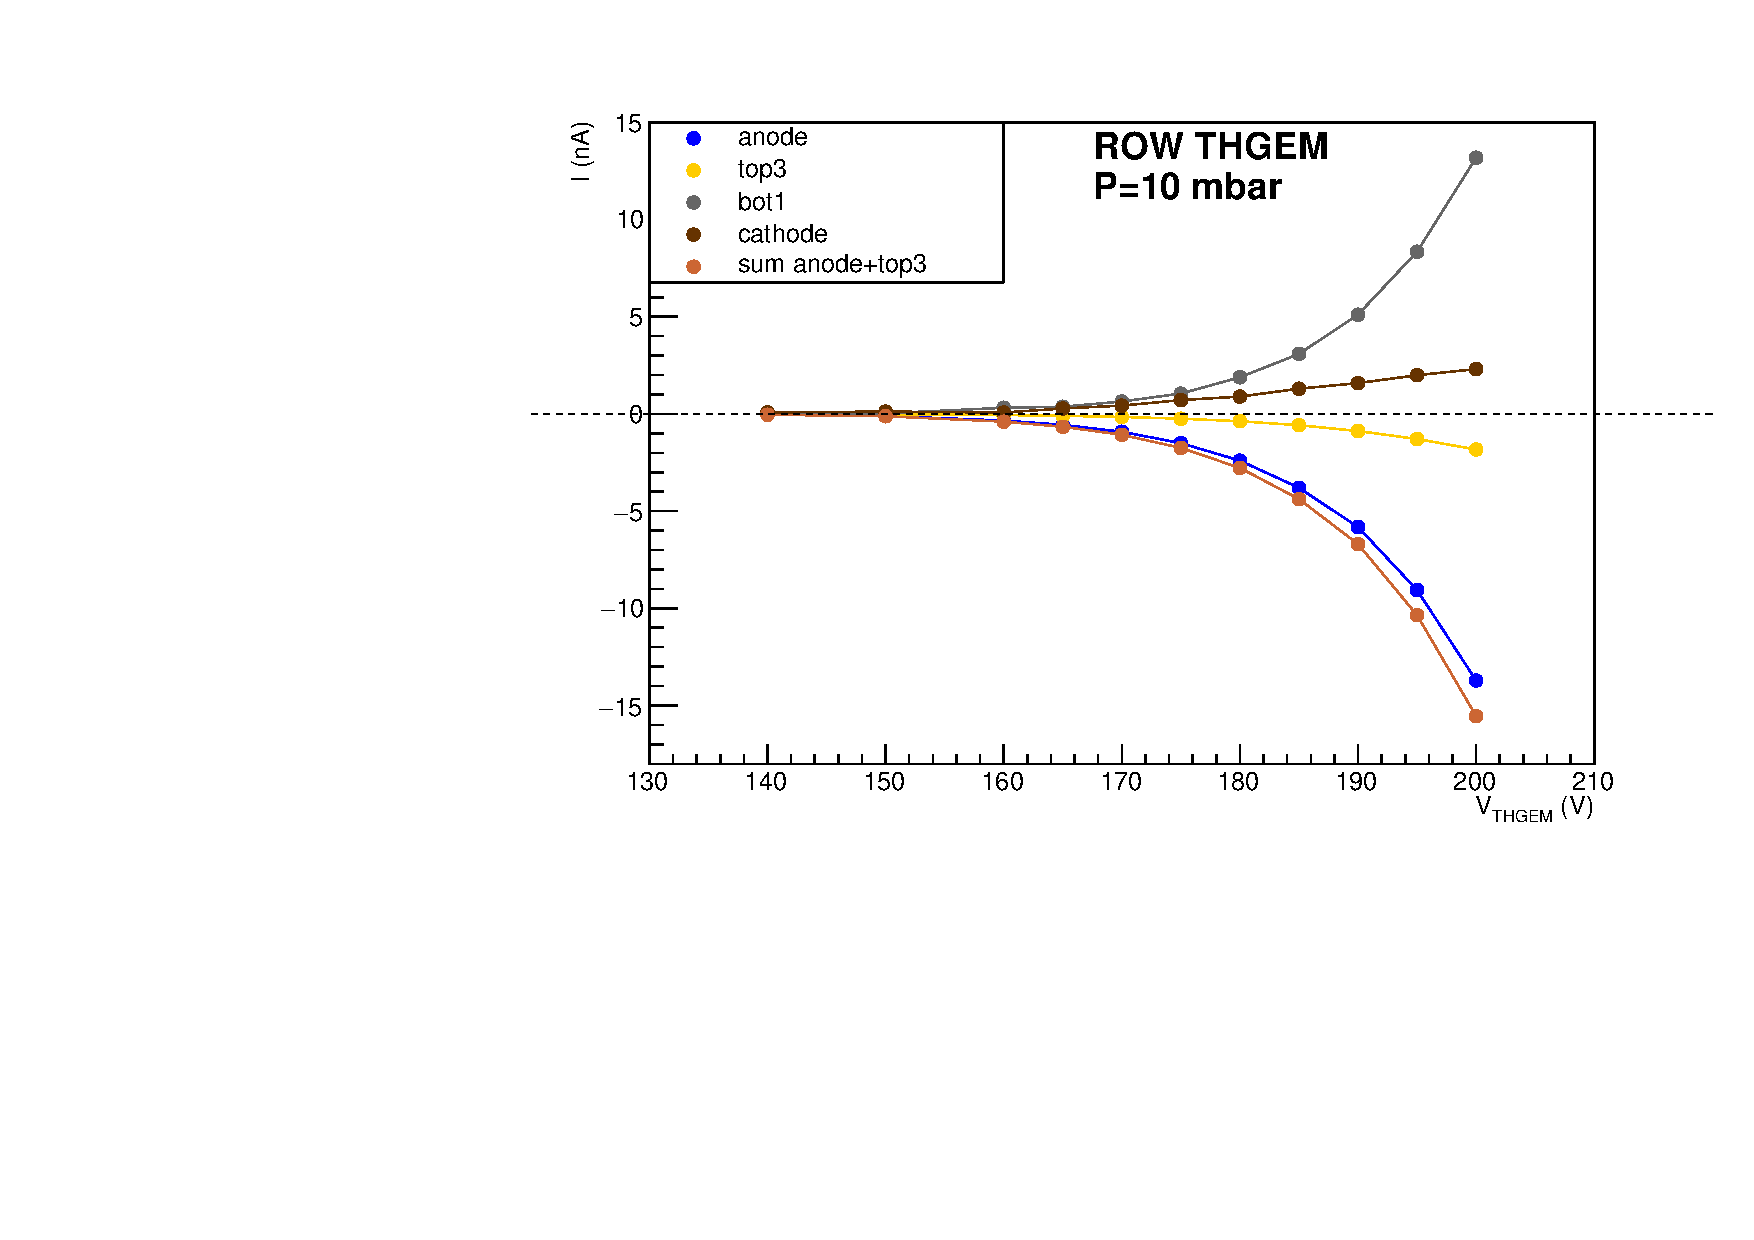
\includegraphics[width=0.96\textwidth]{Immagini/thgemScan_ROW_THGEM_10mbar.pdf}}
	\subfigure[]{ 	\label{fig:thgem_ROWTHGEM_30mbar_bis} 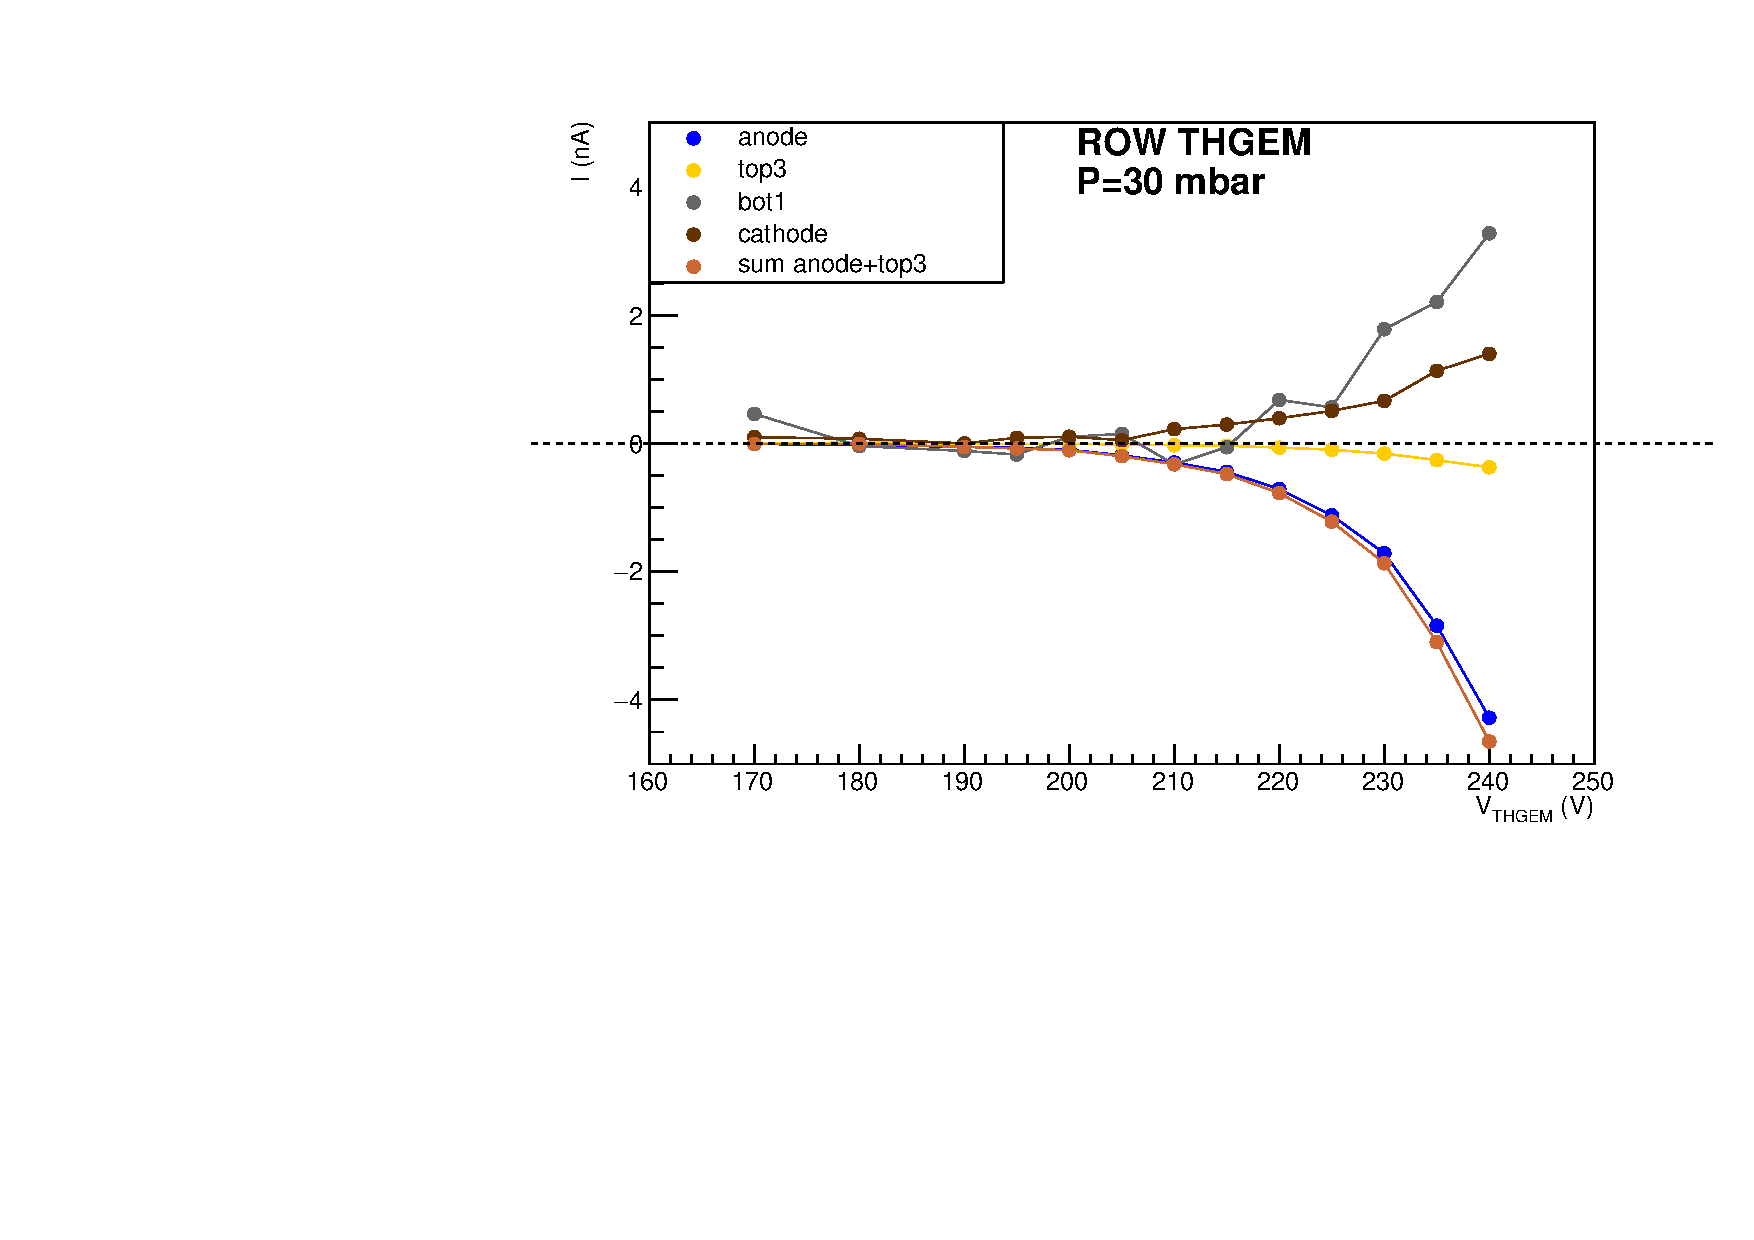
\includegraphics[width=0.96\textwidth]{Immagini/thgemScan_ROW_THGEM_30mbar_bis.pdf}}
	\caption{Currents measured during the scan on the voltage \Vthgem{} across each ROW THGEM: in (a) at 10~mbar, in (b) at 32~mbar.}
	\label{fig:thgem_ROWTHGEM}
\end{figure}


From these measurements, the multiplication factors of the ROW THGEM were evaluated as a function of \Vthgem{} and pressure. 




\begin{figure}[!t]
	\centering
	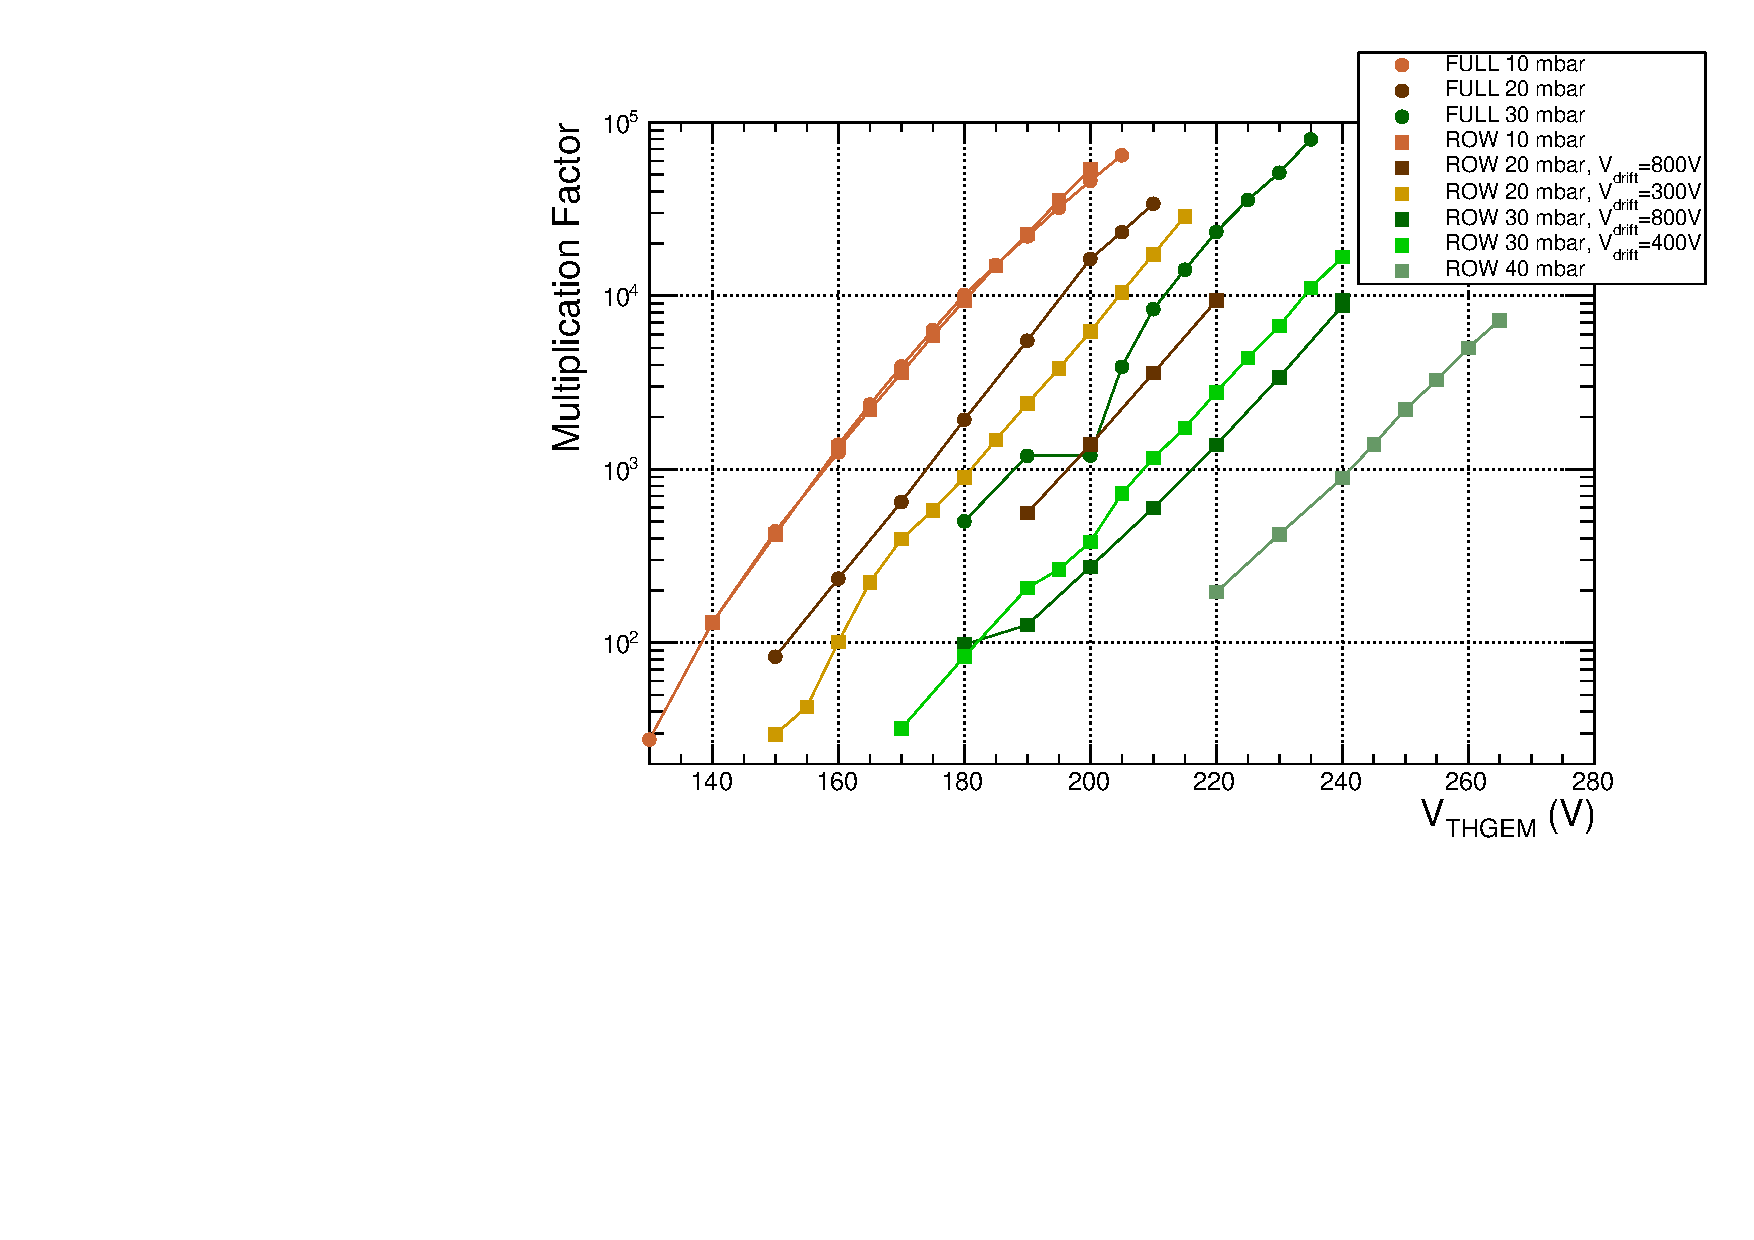
\includegraphics[width=\textwidth]{Immagini/MFvsTHGEM_FULLandROW_bis.pdf}
	\caption{Comparison between the multiplication factors evaluated for the ROW THGEM (square) and those for the FULL THGEM (circle) as a function of \Vthgem{} and pressure.}
	\label{fig:multiplication_factor_FULLandROW}
\end{figure}










\clearpage

\subsubsection{Scan on \Vdrift}

To fully characterize the tracker response, a study was conducted varying the potential difference \Vdrift{} across the drift region, while pressure, \Vind{} and \Vthgem{} were kept fixed.
The explored range goes from 0~V (or 100~V in the case with P~=~20~mbar) to the discharge voltage, which depends on the gas pressure: for P~=~30~mbar it was 1400~V, for P~=~20~mbar it was 1000~V, and for P~=~11~mbar it was 800~V.
The increments were of 100~V for all the cases, but for P~=~11~mbar the first 400~V were scanned in step of 30~V.
In Table~\ref{tab:ROWTHGEM_vdrift} the adopted value of pressure, \Vind{} and \Vthgem{} are shown.


\begin{table} [!h]
	\begin{center}
		\renewcommand{\arraystretch}{1.2}
		\begin{tabular} {ccccc}
			P (mbar) & & \Vind{} (V) & & \Vthgem{} (V)\\
			\toprule[0.1em]
			%\hline
			30	& &	70	& &	240 \\
			30	& &	70	& & 230 \\
			20	& & 80	& & 210 \\
			10	& & 50	& & 180 \\
			
			\bottomrule[0.1em]
		\end{tabular}
	\end{center}
	\caption{The values of pressure (P), \Vind{} and \Vthgem{} adopted for the study on \Vdrift.} \label{tab:ROWTHGEM_vdrift}
\end{table}


The result of the two scans at 30~mbar are shown in Figure~\ref{fig:drift_ROWTHGEM_30mbar_both}: in both cases the measured currents increase rapidly up to 200~V, then they decrease and reach a saturation value. 
\textcolor{red}{Perch�?}


\begin{figure}[!htb]
	\centering
	\subfigure[]{ \label{fig:drift_ROWTHGEM_30mbar} 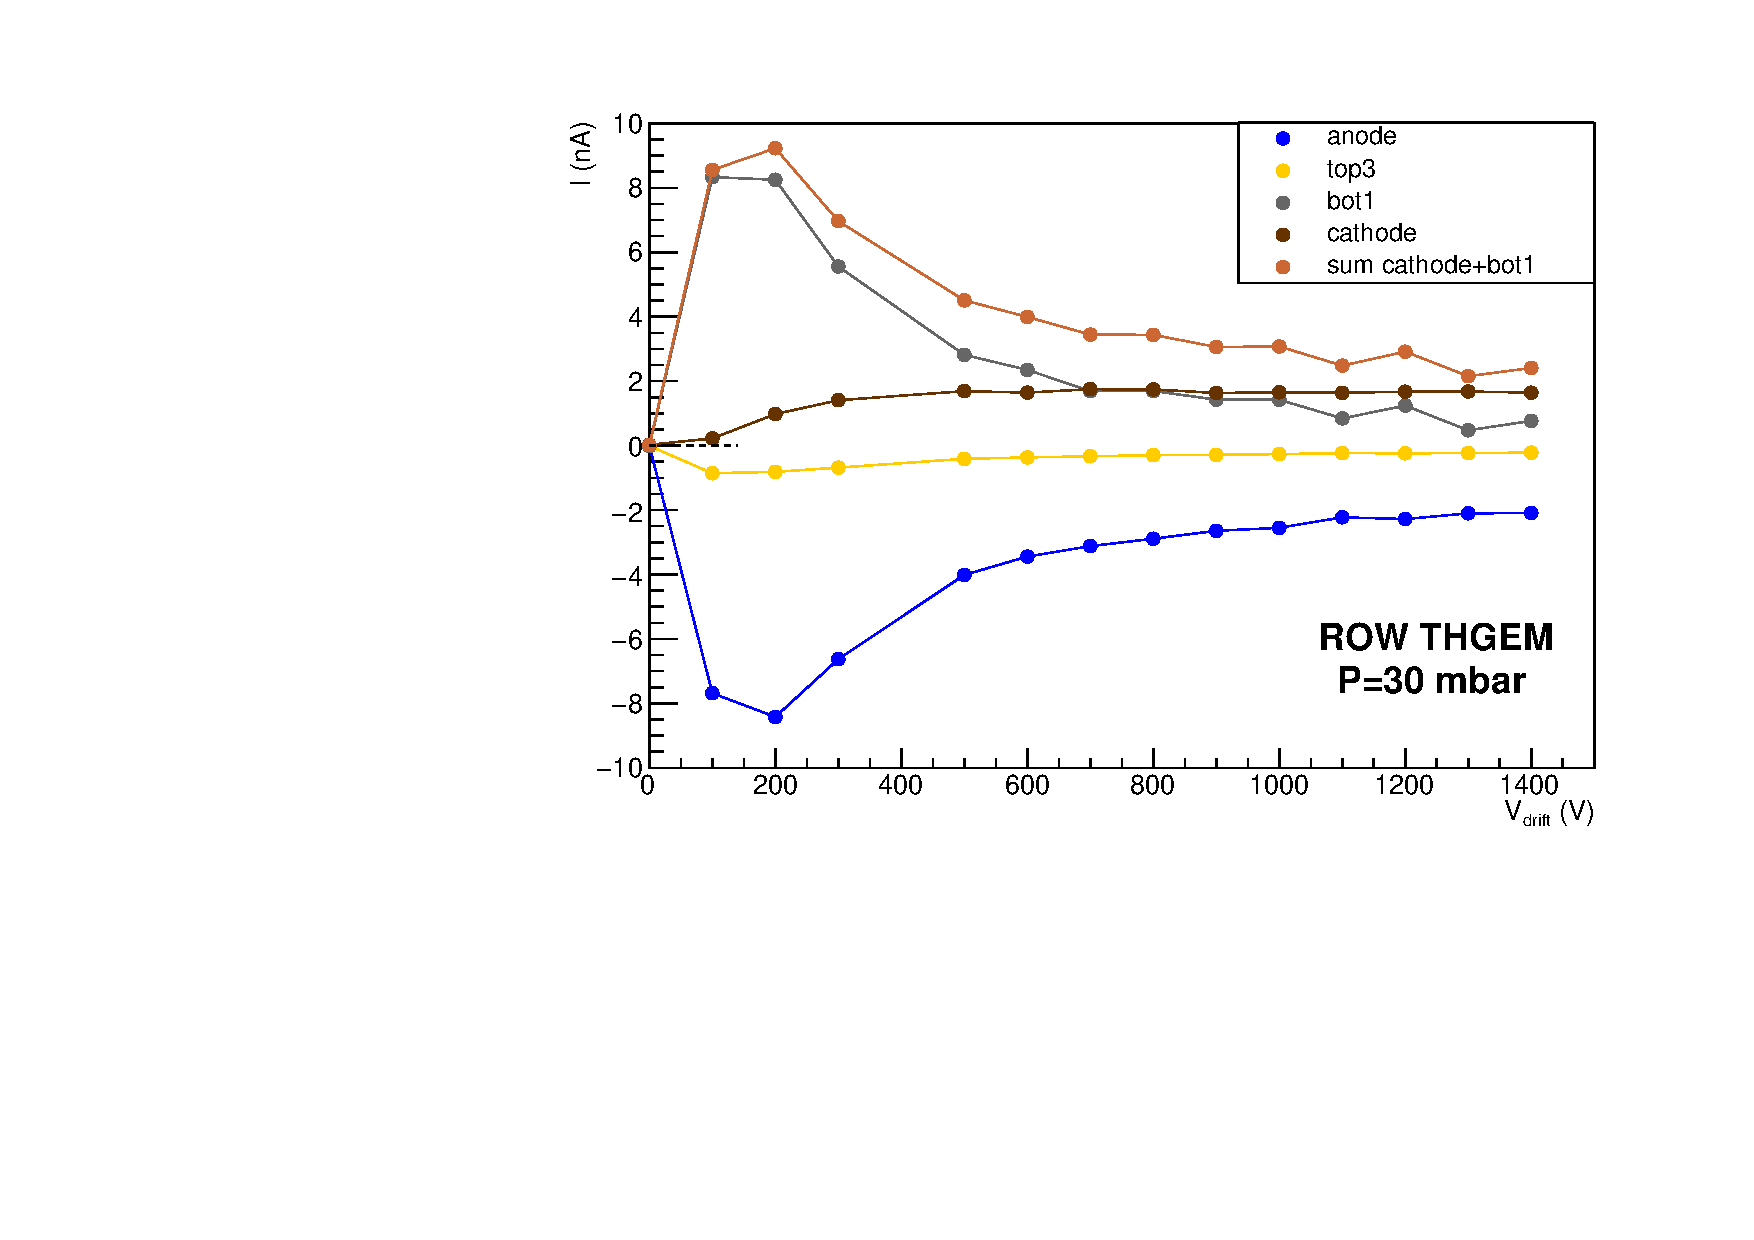
\includegraphics[width=0.96\textwidth]{Immagini/DriftScan_ROW_THGEM_30mbar.pdf}}
	\subfigure[]{ 	\label{fig:drift_ROWTHGEM_30mbar_bis} 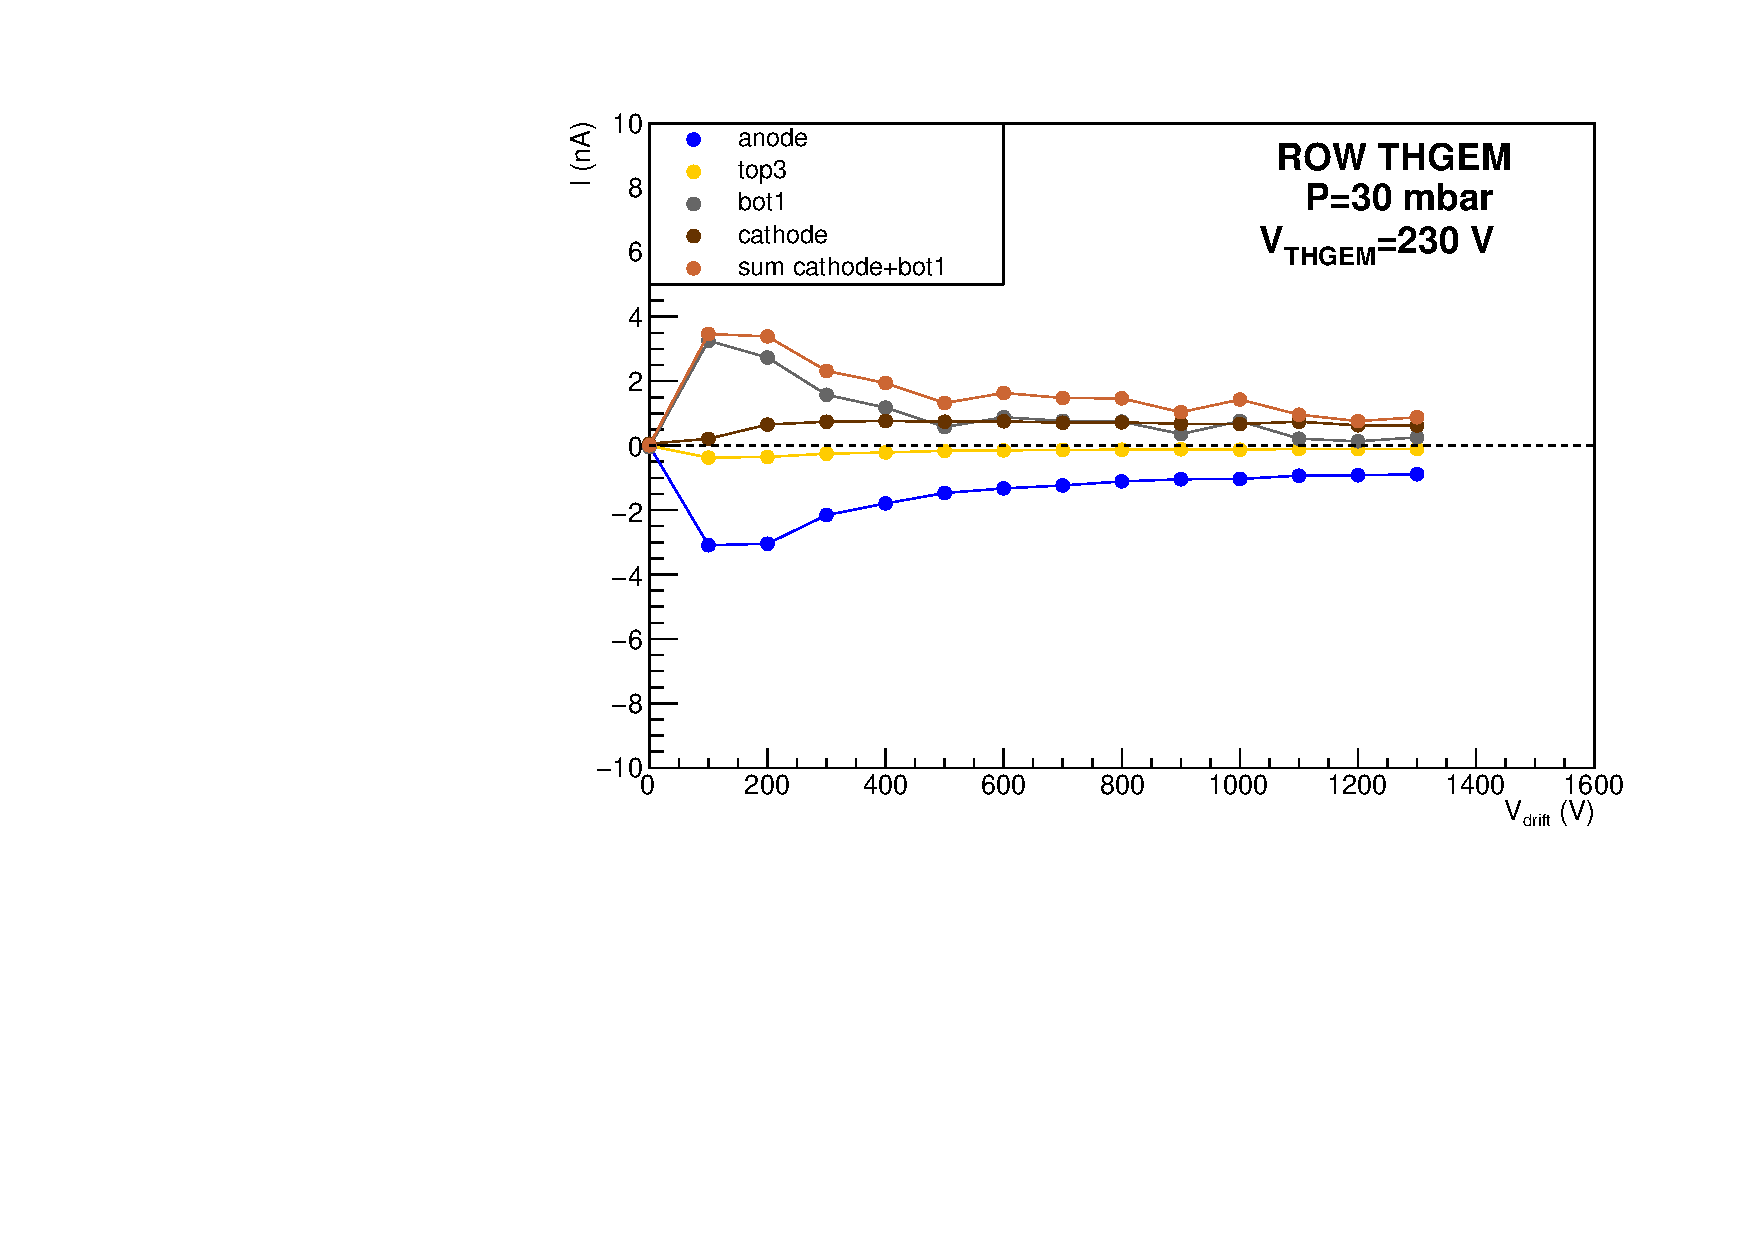
\includegraphics[width=0.96\textwidth]{Immagini/DriftScan_ROW_THGEM_30mbar_bis.pdf}}
	\caption{Currents measured during the scan on the voltage \Vdrift{} across the drift region at 20~mbar: in (a) \Vthgem{} is at 240~V, in (b) it is at 230~V.}
	\label{fig:drift_ROWTHGEM_30mbar_both}
\end{figure}

The same phenomenon appears also in the scans at 20 and 10~mbar, respectively shown in Figure~\ref{fig:drift_ROWTHGEM_20mbar} and~\ref{fig:drift_ROWTHGEM_10mbar}.

\begin{figure}[!htb]
	\centering
	\subfigure[]{ \label{fig:drift_ROWTHGEM_20mbar} 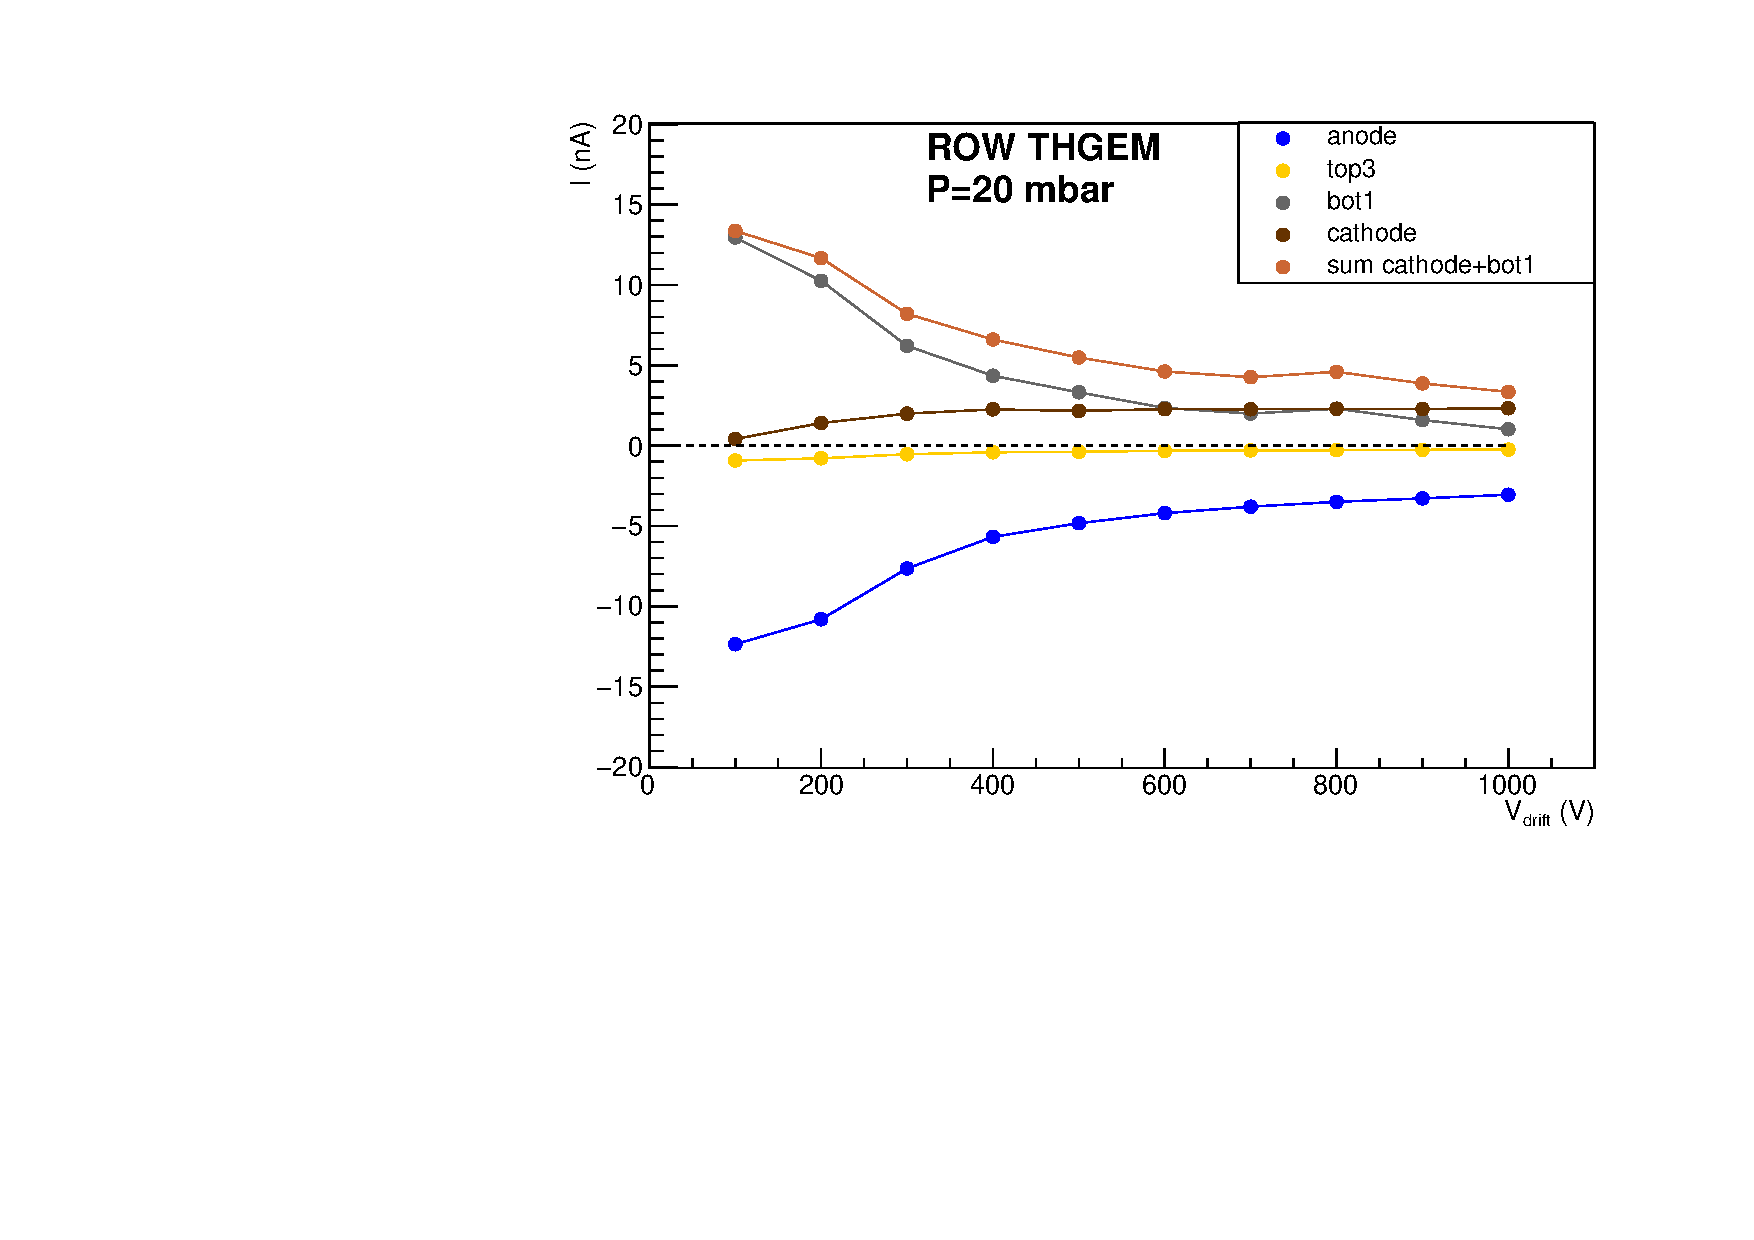
\includegraphics[width=0.96\textwidth]{Immagini/DriftScan_ROW_THGEM_20mbar.pdf}}
	\subfigure[]{ 	\label{fig:drift_ROWTHGEM_10mbar} 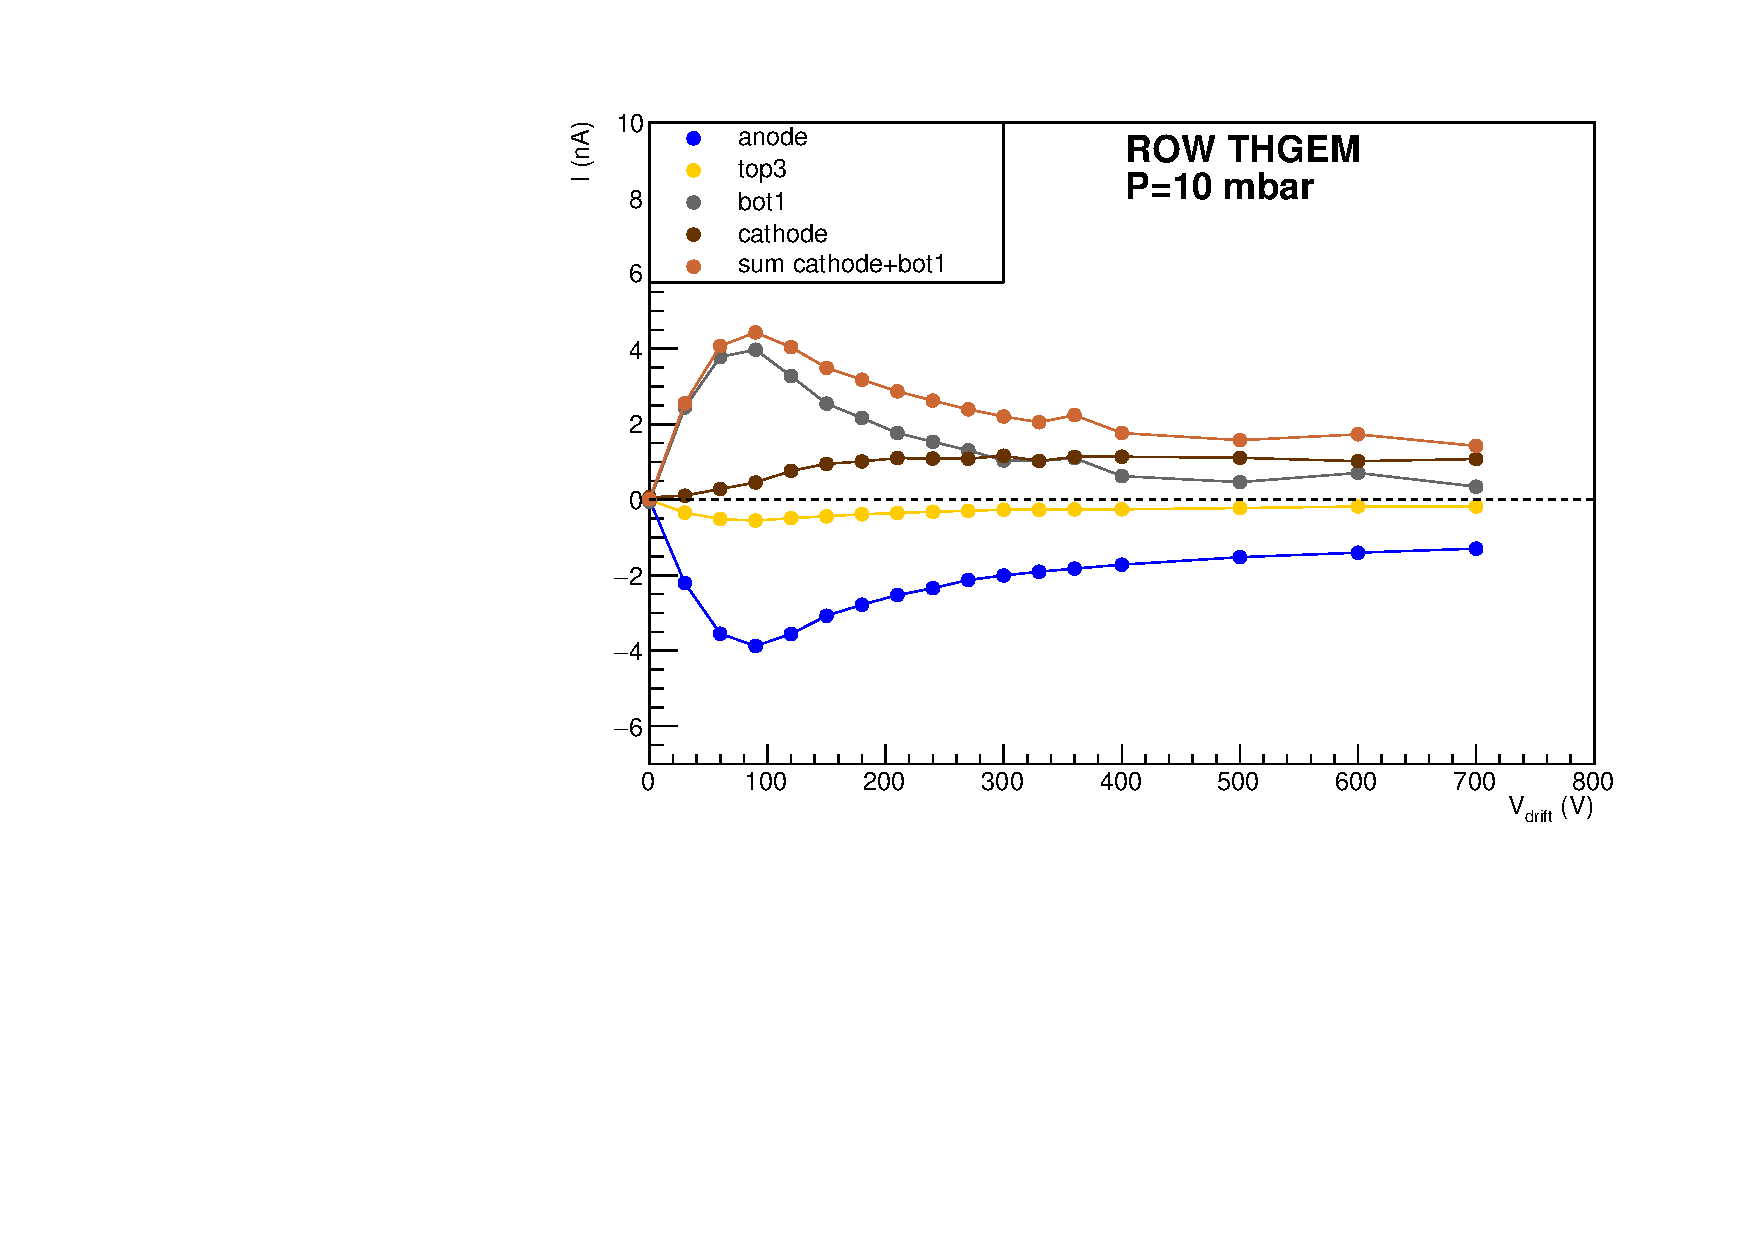
\includegraphics[width=0.96\textwidth]{Immagini/DriftScan_ROW_THGEM_10mbar.pdf}}
	\caption{Currents measured during the scan on the voltage \Vdrift{} across the drift region: in (a) at 20~mbar, in (b) at 10~mbar.}
	\label{fig:drift_ROWTHGEM_20and10_mbar}
\end{figure}



From these measurements, the ion backflow of the ROW THGEM was evaluated as a function of \Vdrift{} and pressure.
The results of the calculation are shown in Figure~\ref{fig:ion_backflow_FULLandROW}: the ion backflow rapidly increases at increasing \Vdrift{} and is much bigger than that of the FULL THGEM.





\begin{figure}[htbp]
	\centering
	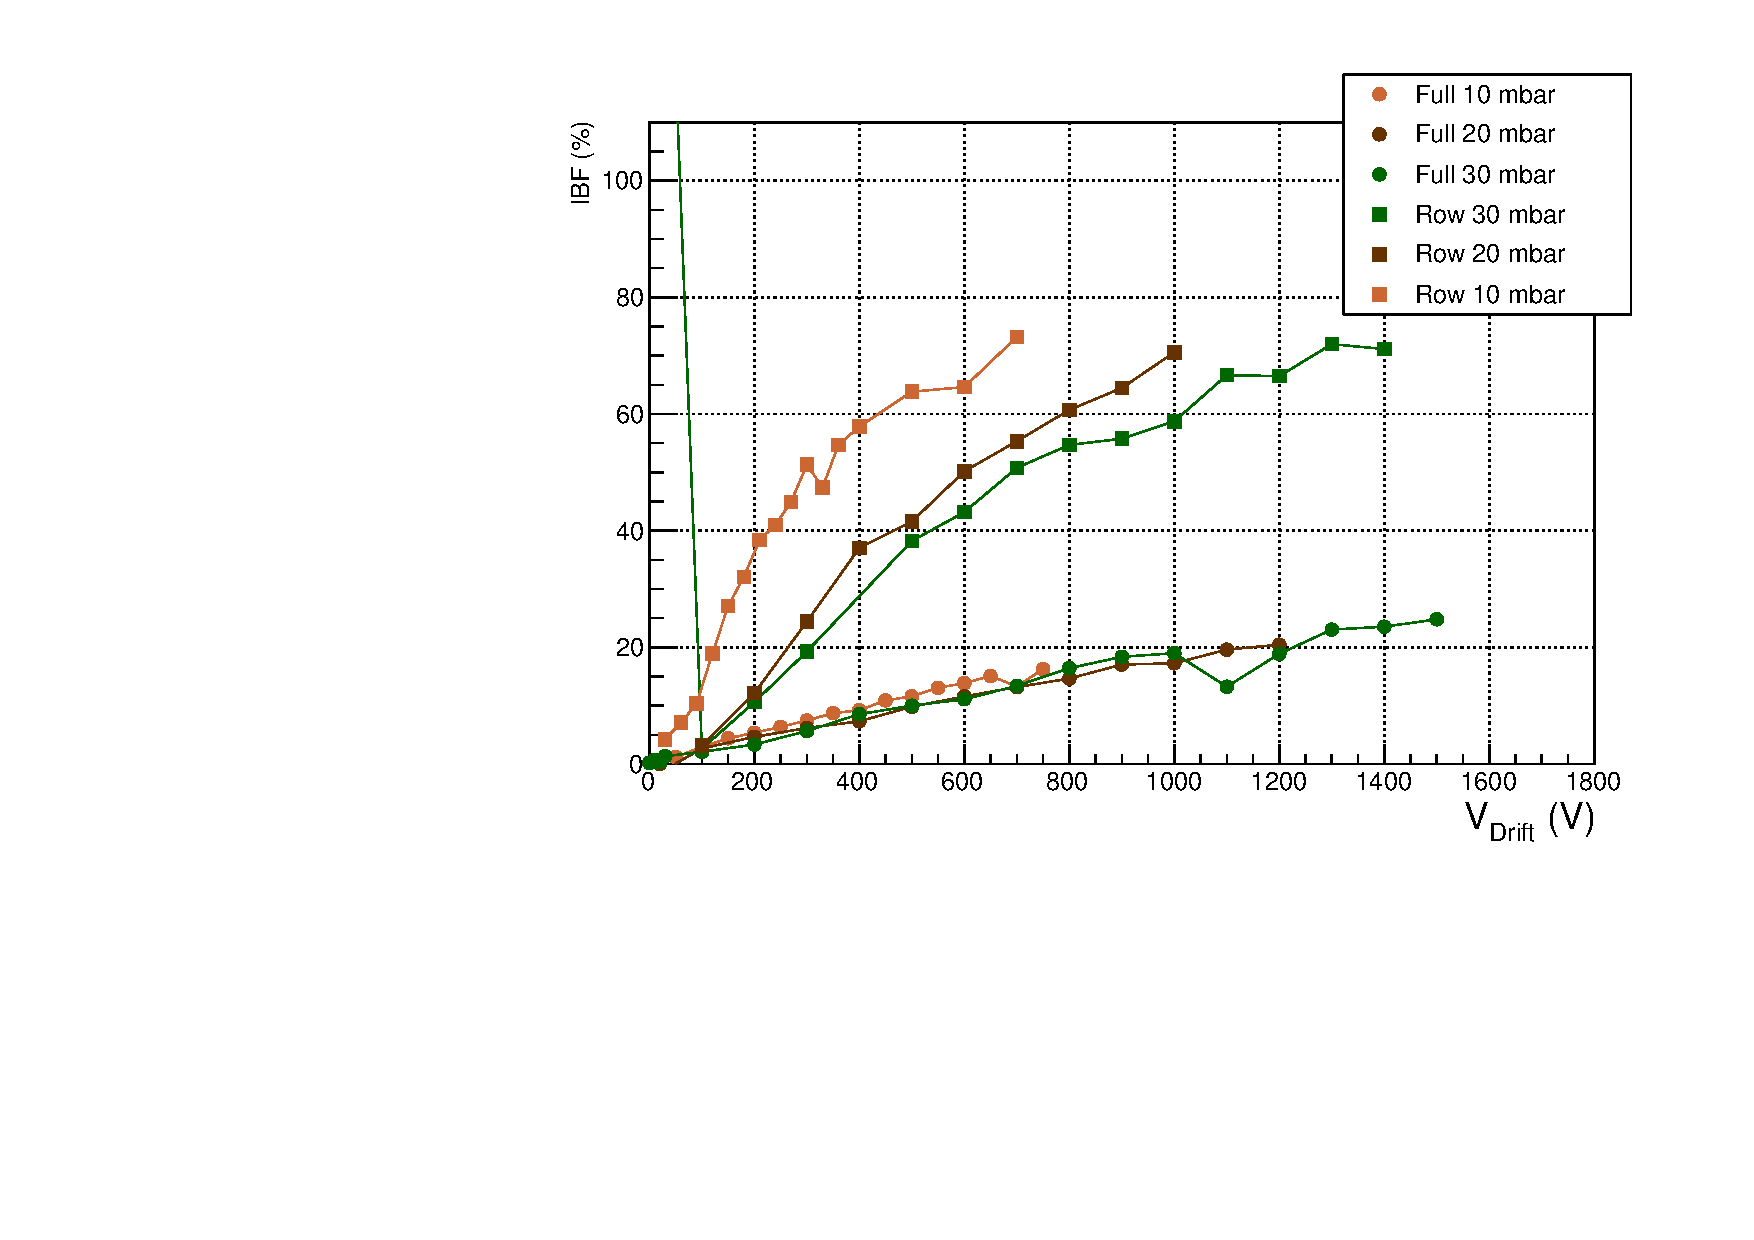
\includegraphics[width=\textwidth]{Immagini/IBFvsDrift_FULLandROW.pdf}
	\caption{Comparison between the ion backflows evaluated for the ROW THGEM (square) and those for the FULL THGEM (circle) as a function of \Vdrift{} and pressure.}
	\label{fig:ion_backflow_FULLandROW}
\end{figure}







\clearpage


\subsection{First test with beam}

The first test with beam was on February 19 2020. We tested FULL THGEM \textit{F10} at 60 pA, 400 pA, 1 nA and 1.8 nA of beam current. The pressure was 9.4 mbar.

\subsubsection{Scan on \Vthgem}

The measurement was made fixing \Vind{} = 50 V and \Vdrift{} = 400 V. The currents have the same behaviour of the scan on \Vthgem{} with alpha source ~\ref{fig:thgem_FULLTHGEM_10mbar_bis}. The discharge was at \Vthgem{} = 190 V with beam instead of \Vthgem{} = 210 V with alpha source. Another important difference is the maximum anodic achievable current: ~20 nA with alpha souce, ~120 nA with 60 pA and ~280 nA with 400 pA of beam current ~\ref{fig:thgemScan_THGEM10_beam_10mbar}.

\begin{figure}[!htb]
	\centering
	\subfigure[]{ \label{fig:thgemScan_THGEM10_60pA_10mbar} 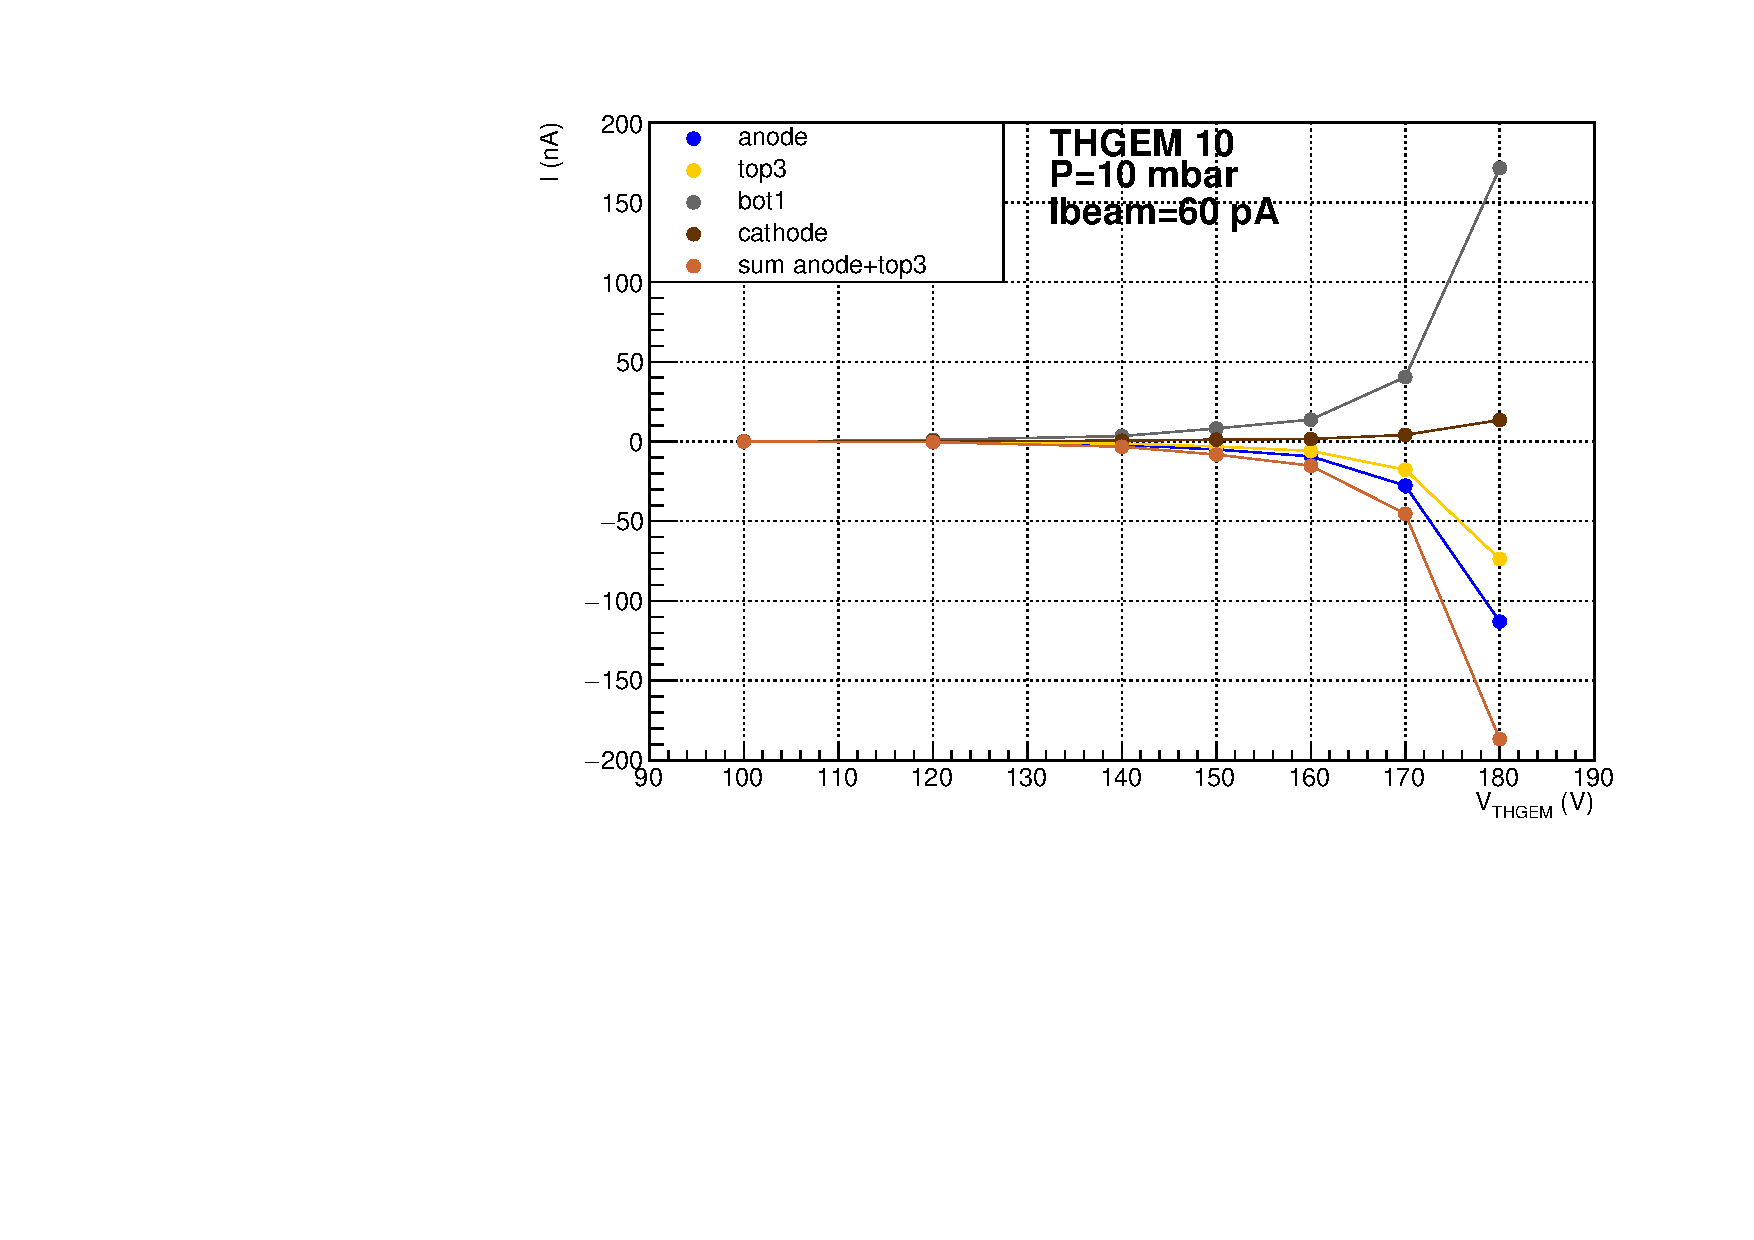
\includegraphics[width=0.96\textwidth]{Immagini/thgemScan_THGEM10_60pA_10mbar.pdf}}
	\subfigure[]{ 	\label{fig:thgemScan_THGEM10_400pA_10mbar} 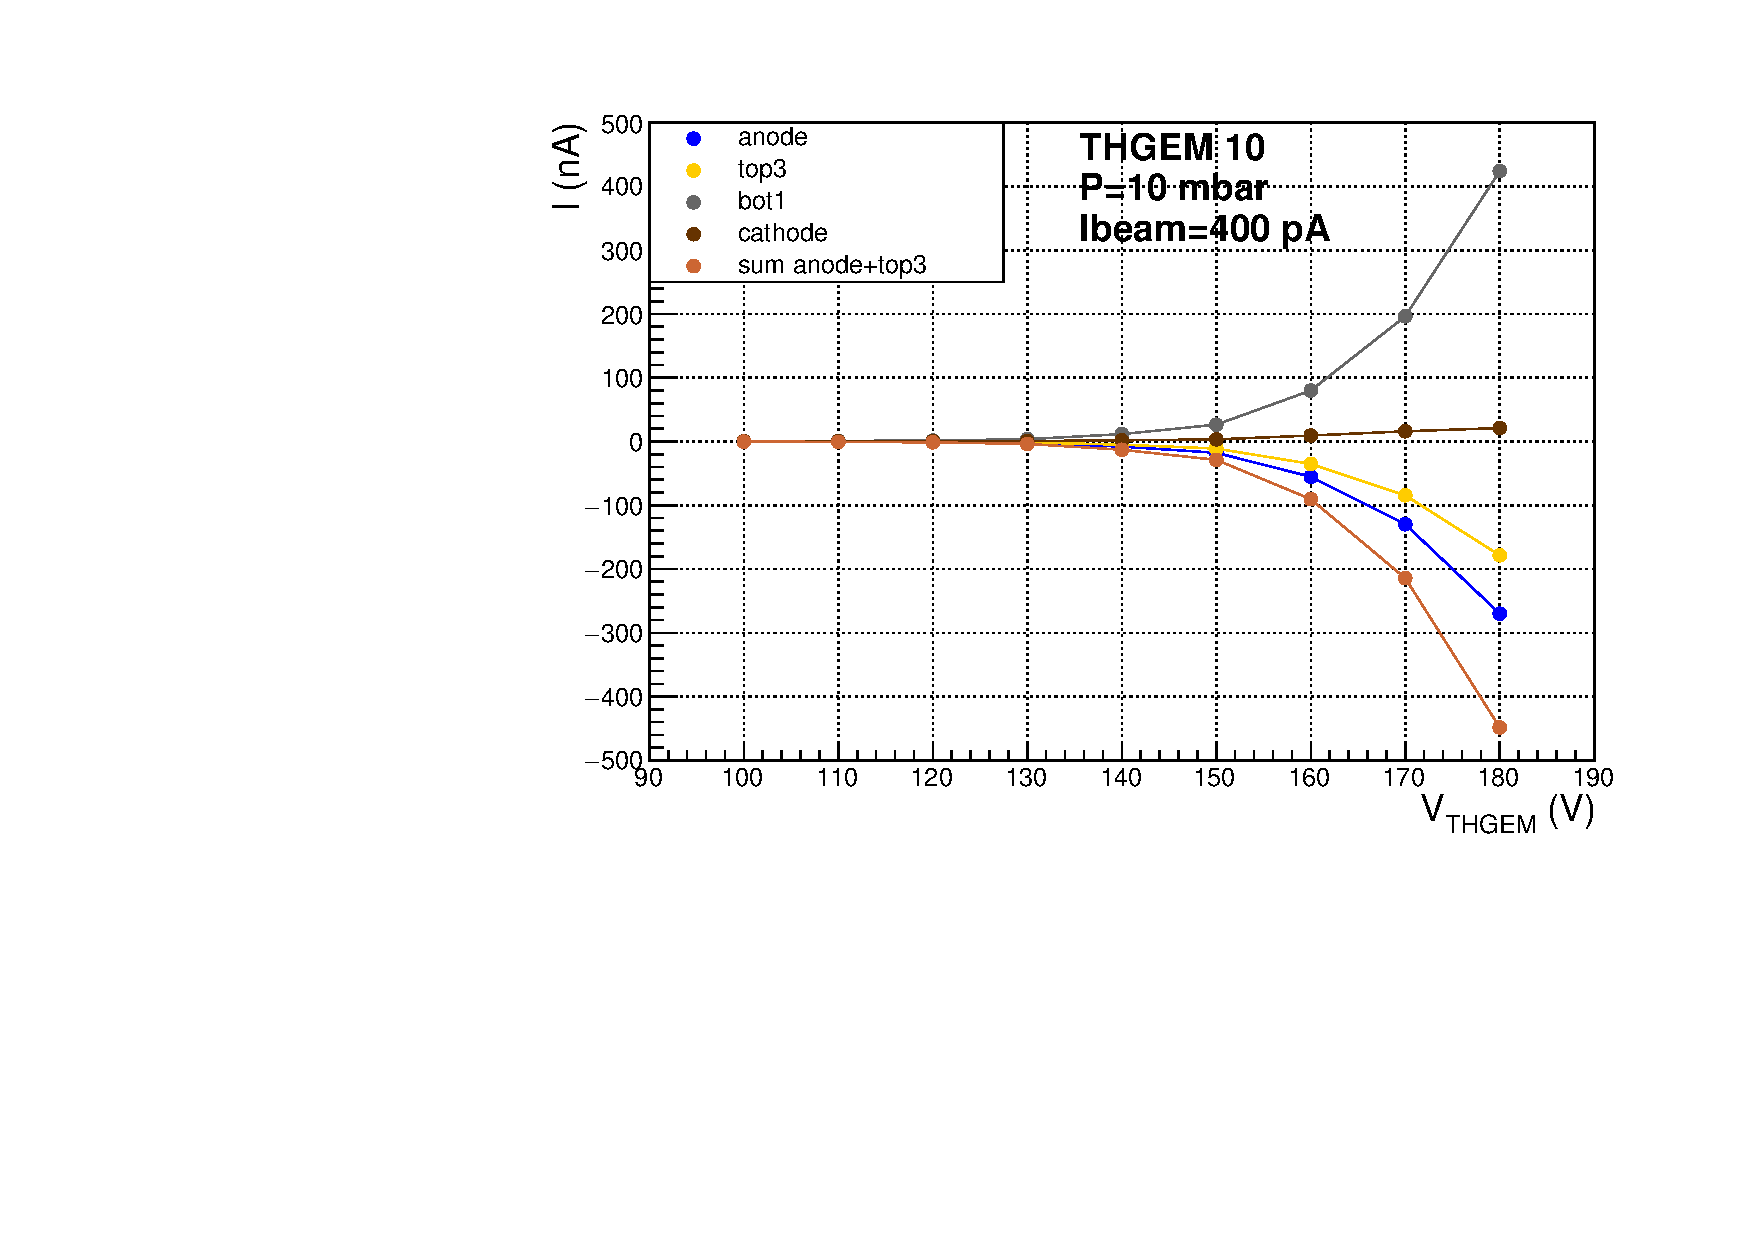
\includegraphics[width=0.96\textwidth]{Immagini/thgemScan_THGEM10_400pA_10mbar.pdf}}
	\caption{Currents measured during the scan on the voltage \Vthgem{} across each FULL THGEM fixing \Vind{} = 50 V and \Vdrift{} = 400 V: in (a) at 60 pA, in (b) at 400 pA.}
	\label{fig:thgemScan_THGEM10_beam_10mbar}
\end{figure}

\subsubsection{Scan on \Vdrift}

The measurement was made fixing \Vind{} = 50 V and \Vthgem{} = 160 V. The currents have the same behaviour of the scan on \Vdrift{} with alpha source ~\ref{fig:driftScan_THGEM10_alpha_10mbar}. The discharge was at \Vdrift{} = 800 V with beam instead of more than \Vdrift{} = 700 V with alpha source. Another important difference is the maximum anodic achievable current: ~-0.5 nA with alpha souce, ~-20 nA with 60 pA and ~-55 nA with 400 pA of beam current.

\begin{figure}[!htb]
	\centering
	\subfigure[]{ \label{fig:driftScan_THGEM10_60pA_10mbar} 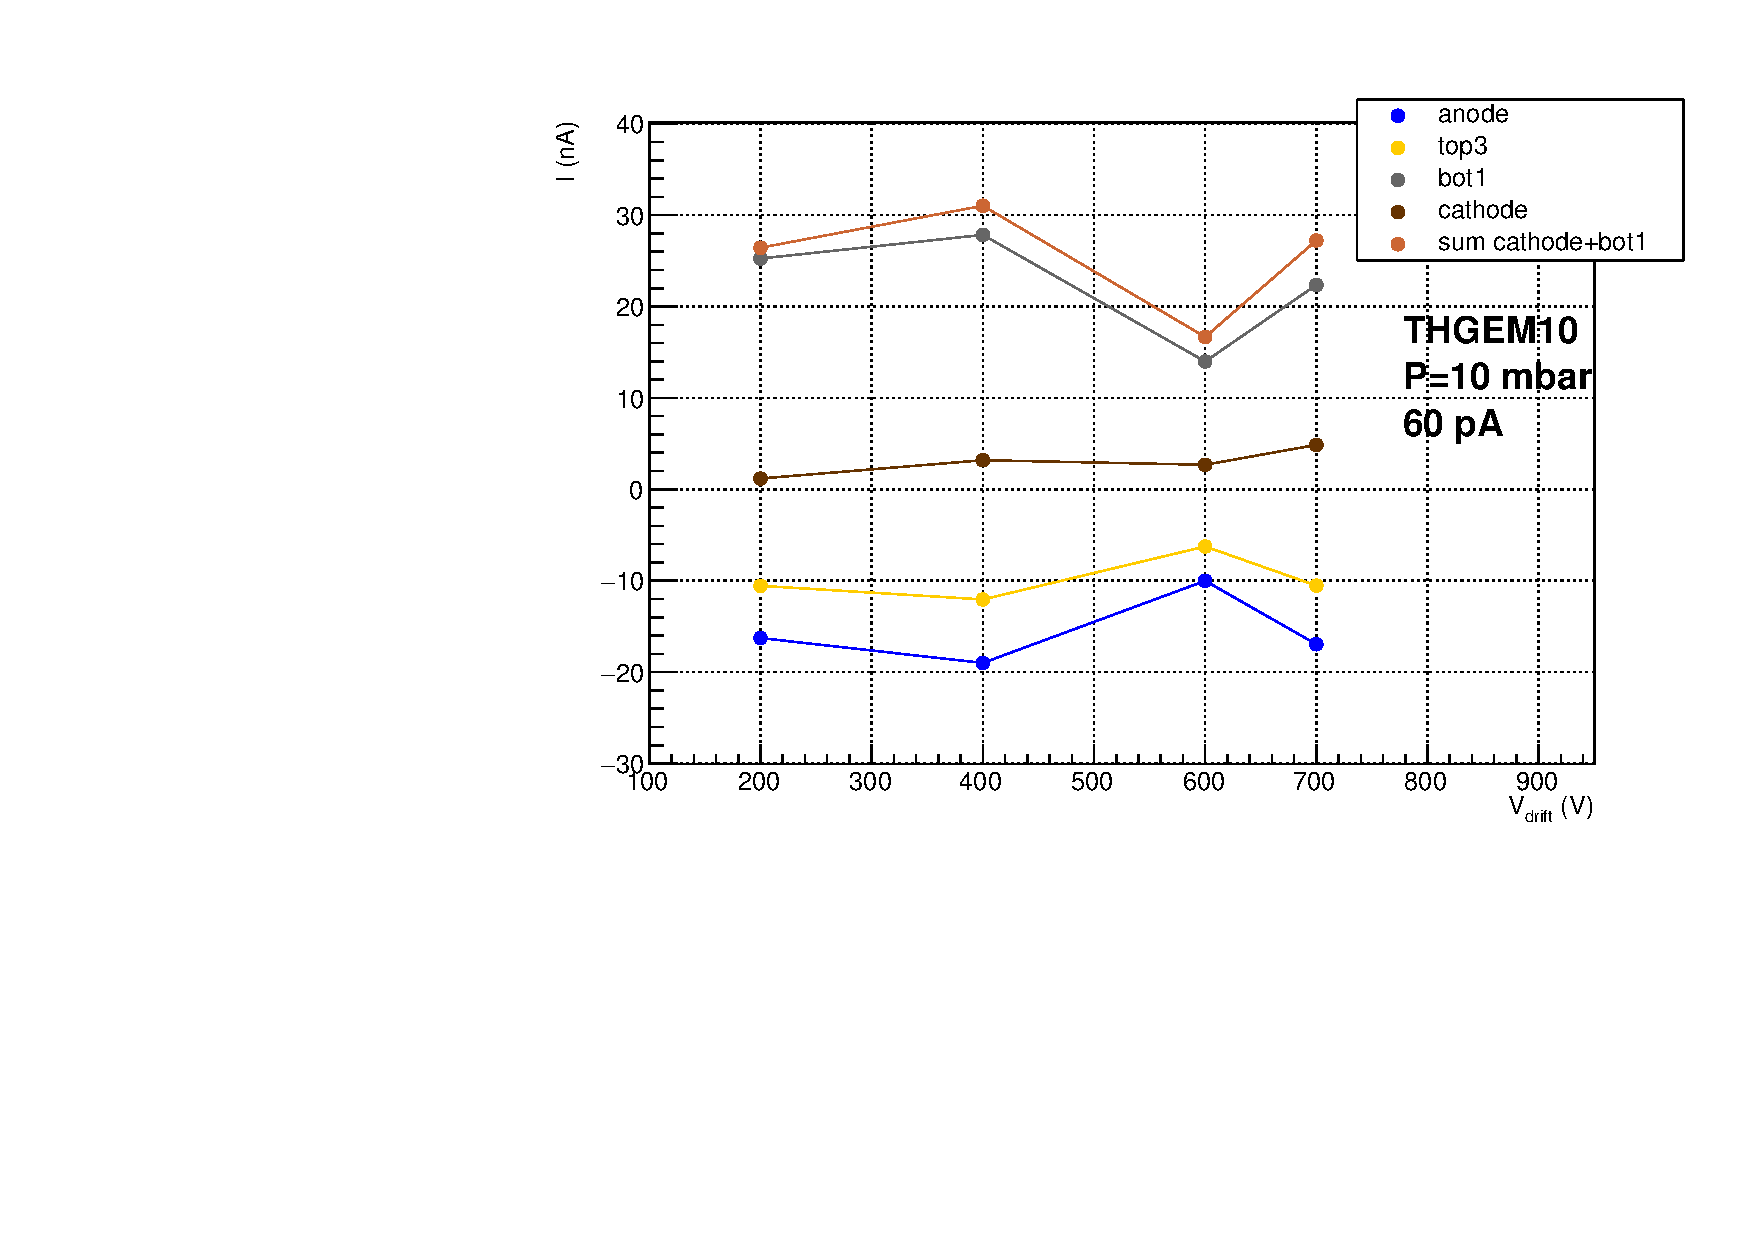
\includegraphics[width=0.96\textwidth]{Immagini/driftScan_THGEM10_60pA_10mbar.pdf}}
	\subfigure[]{ 	\label{fig:driftScan_THGEM10_400pA_10mbar} 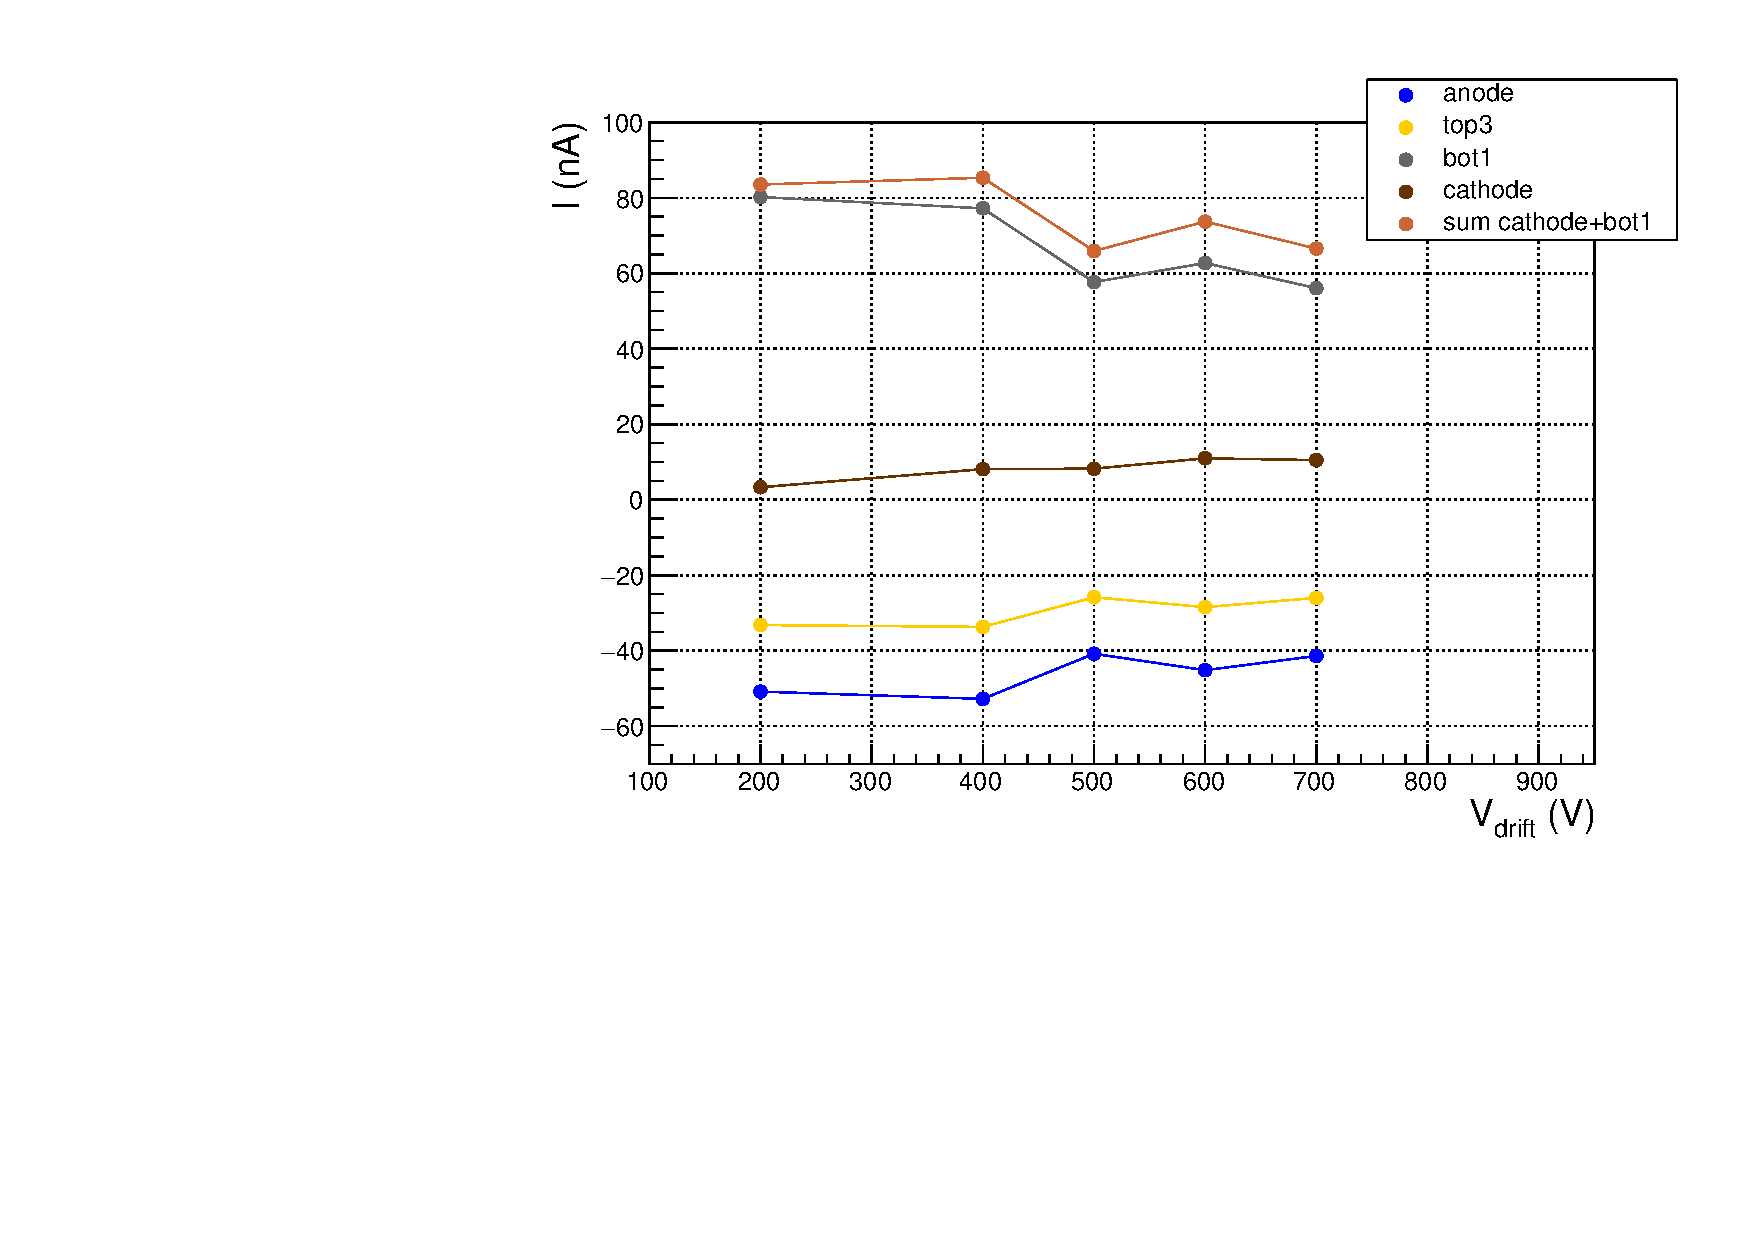
\includegraphics[width=0.96\textwidth]{Immagini/driftScan_THGEM10_400pA_10mbar.pdf}}
	\caption{Currents measured during the scan on the voltage \Vdrift{} across each FULL THGEM fixing \Vind{} = 50 V and \Vthgem{} = 160 V: in (a) at 60 pA, in (b) at 400 pA.}
	\label{fig:driftScan_THGEM10_beam_10mbar}
\end{figure}

\subsubsection{Ion Backflows (IBF)}

Looking at figure~\ref{fig:IBFvsDrift_withBeam} we can evaluate IBF behavior increasing \Vdrift{}. IBF increase linear until \Vdrift{} = 600 V. After this point it seems to get a plateau but to be sure it is needed to encrease \Vdrift{}in next measurement.\\

\begin{figure}[htbp]
	\centering
	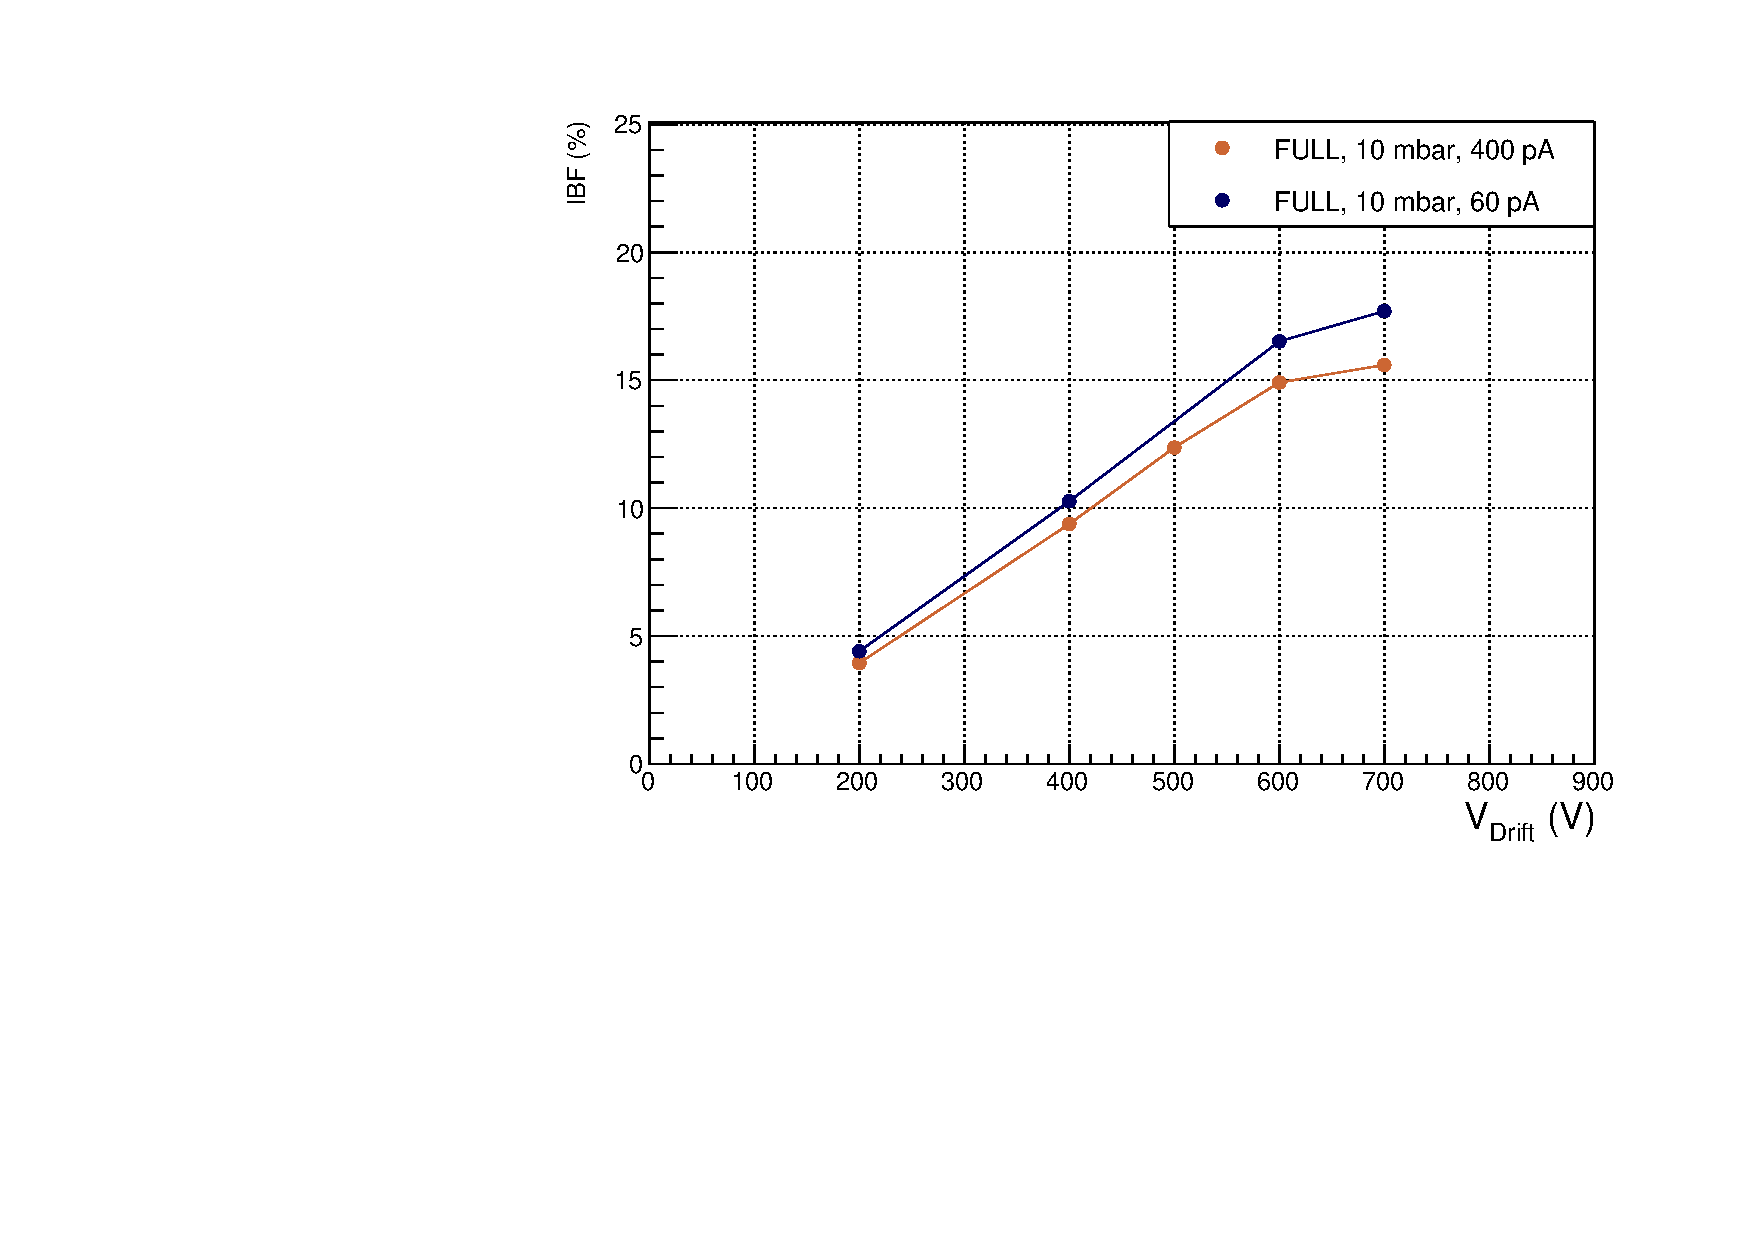
\includegraphics[width=\textwidth]{Immagini/IBFvsDrift_withBeam.pdf}
	\caption{Ion backflows evaluated for FULL THGEM as a function of \Vdrift{} at 60 pA and 400 pA fixing \Vind{} = 50 V and \Vthgem{} = 160 V.}
	\label{fig:IBFvsDrift_withBeam}
\end{figure}



In figure~\ref{fig:IBFvsDrift_beam_alpha_average} IBF was setted as a function of \Vdrift{}. The IBF behaviour for 60 pA, 400 pA at \Vthgem{} = 160 V and alpha source at \Vthgem{} = 190 V with a maximum IBF = 17\%. When \Vthgem{} is less than 190 V the catode current is so small that IBF estimate is not reliable. IBF as a function of \Vdrift{} is not sensible to the rate because it has a costant rise with aplha source and with beam. From the circle points it seems that increasing the beam current (fixed \Vthgem{} = 150 V) the IBF decrease, this behavior cannot be explained. Looking at the blue and red circle points IBF decrease increasing \Vthgem{} with the same beam current.\\

\begin{figure}[htbp]
	\centering
	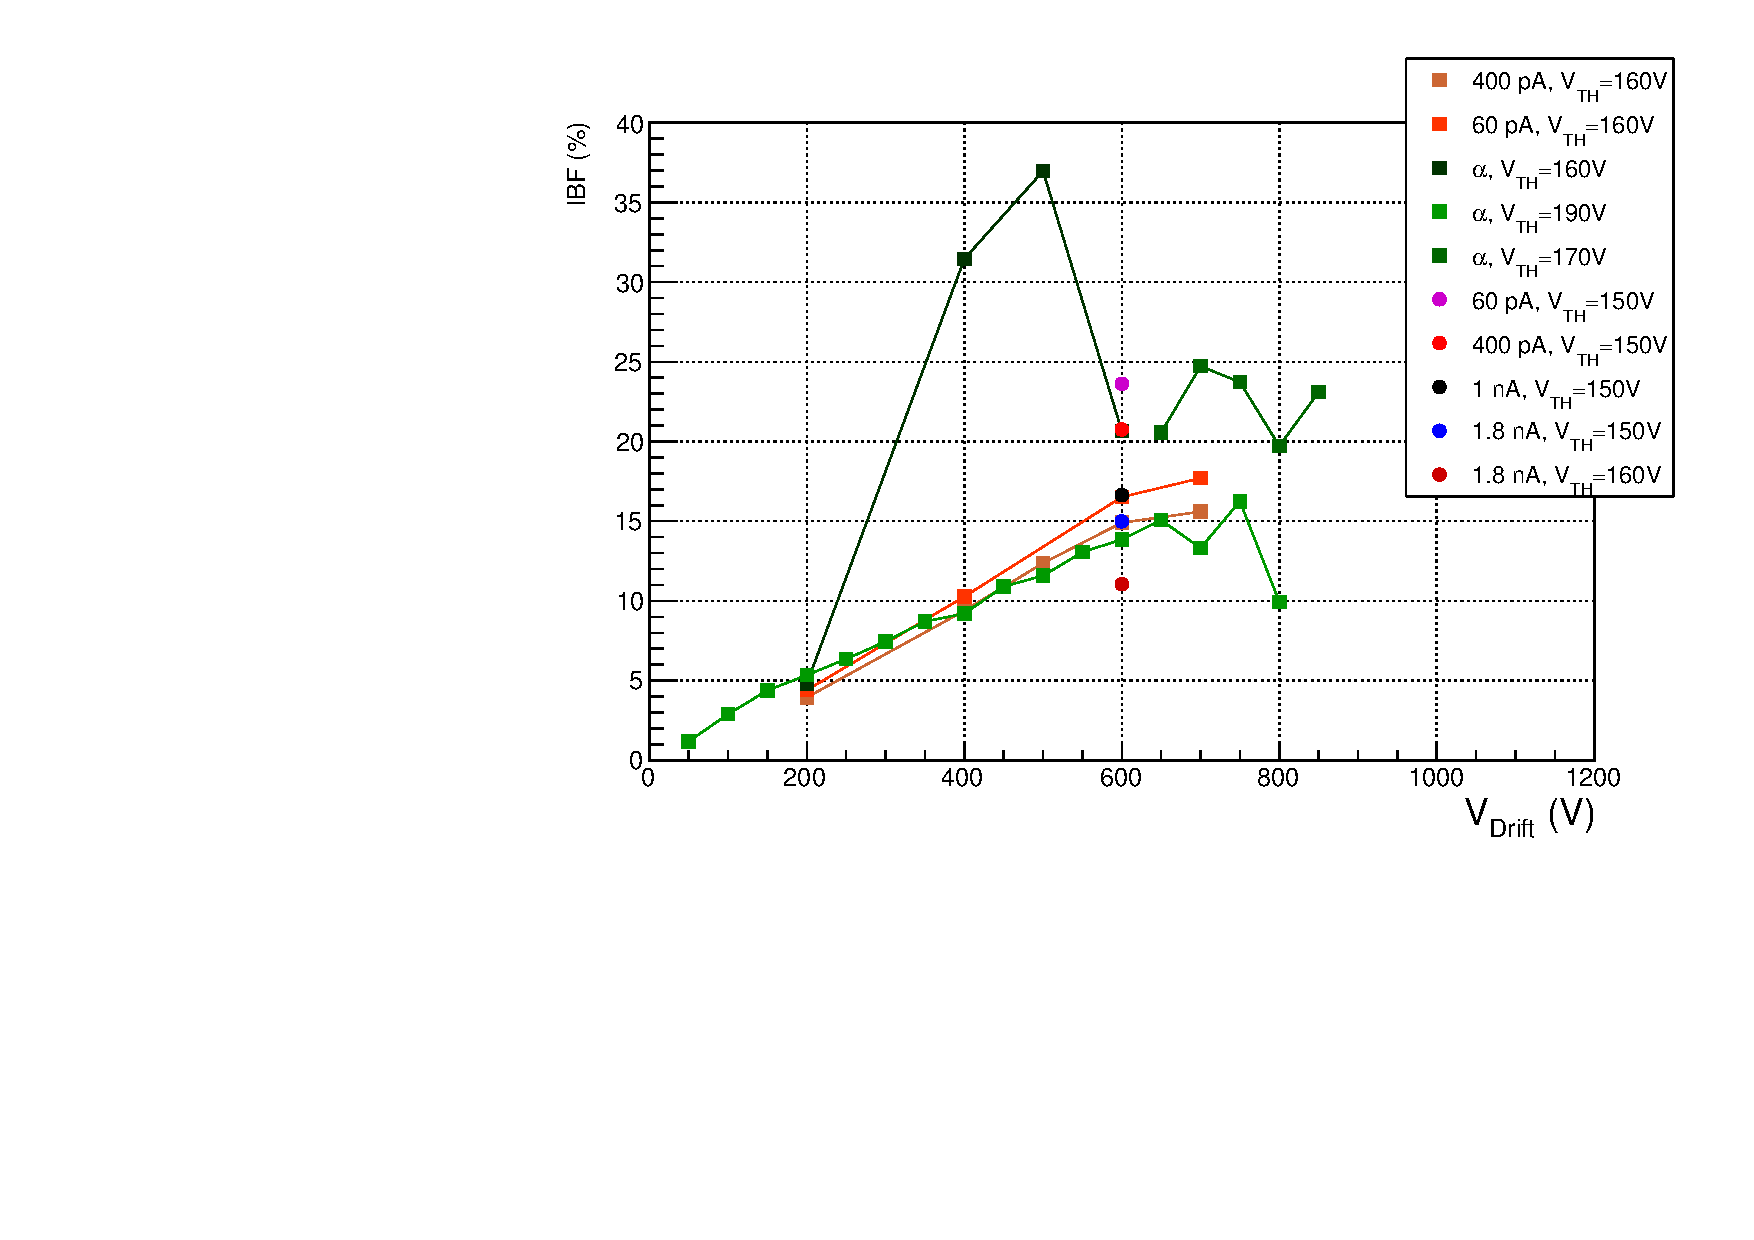
\includegraphics[width=\textwidth]{Immagini/IBFvsDrift_beam_alpha_average.pdf}
	\caption{Ion backflows evaluated for FULL THGEM as a function of \Vdrift{} at 60 pA, 400 pA, 1 nA, 1.8 nA and with alpha source.}
	\label{fig:IBFvsDrift_beam_alpha_average}
\end{figure}


From \Vthgem{} = 100 V to \Vthgem{} = 140 V IBF decrease rapidly, between \Vthgem{} = 140 V and \Vthgem{} = 205 V IBF is nearly constant as visible in figure~\ref{fig:IBFvsTHGEM_beam_alpha}. The best condition to have IBF as less as possible is to work near \Vthgem{} = 200 V but as far as possible from discharge.\\


\begin{figure}[!htb]
	\centering
	\subfigure[]{ \label{fig:IBFvsTHGEM_beam_alpha} 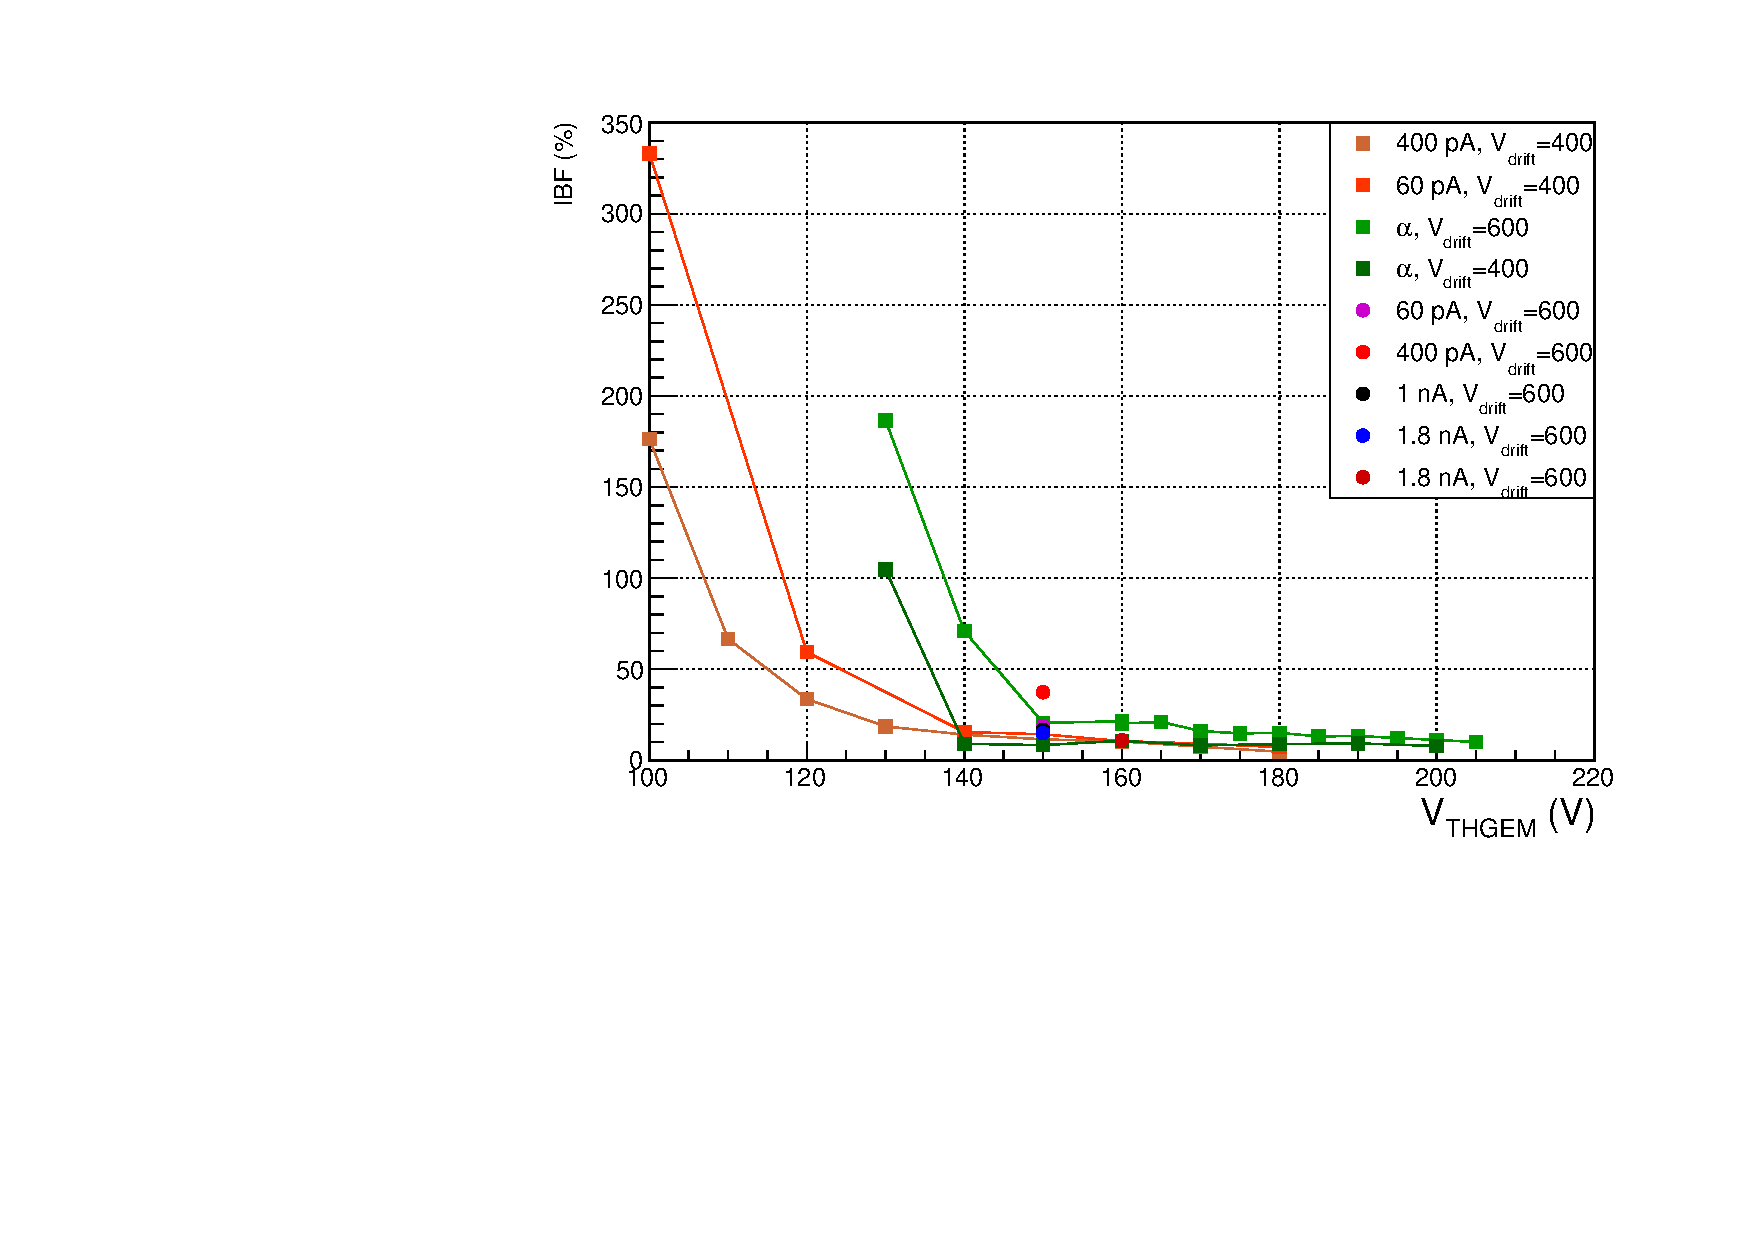
\includegraphics[width=0.96\textwidth]{Immagini/IBFvsTHGEM_beam_alpha.pdf}}
	\subfigure[]{ 	\label{fig:IBFvsTHGEM_beam_alpha_zoom} 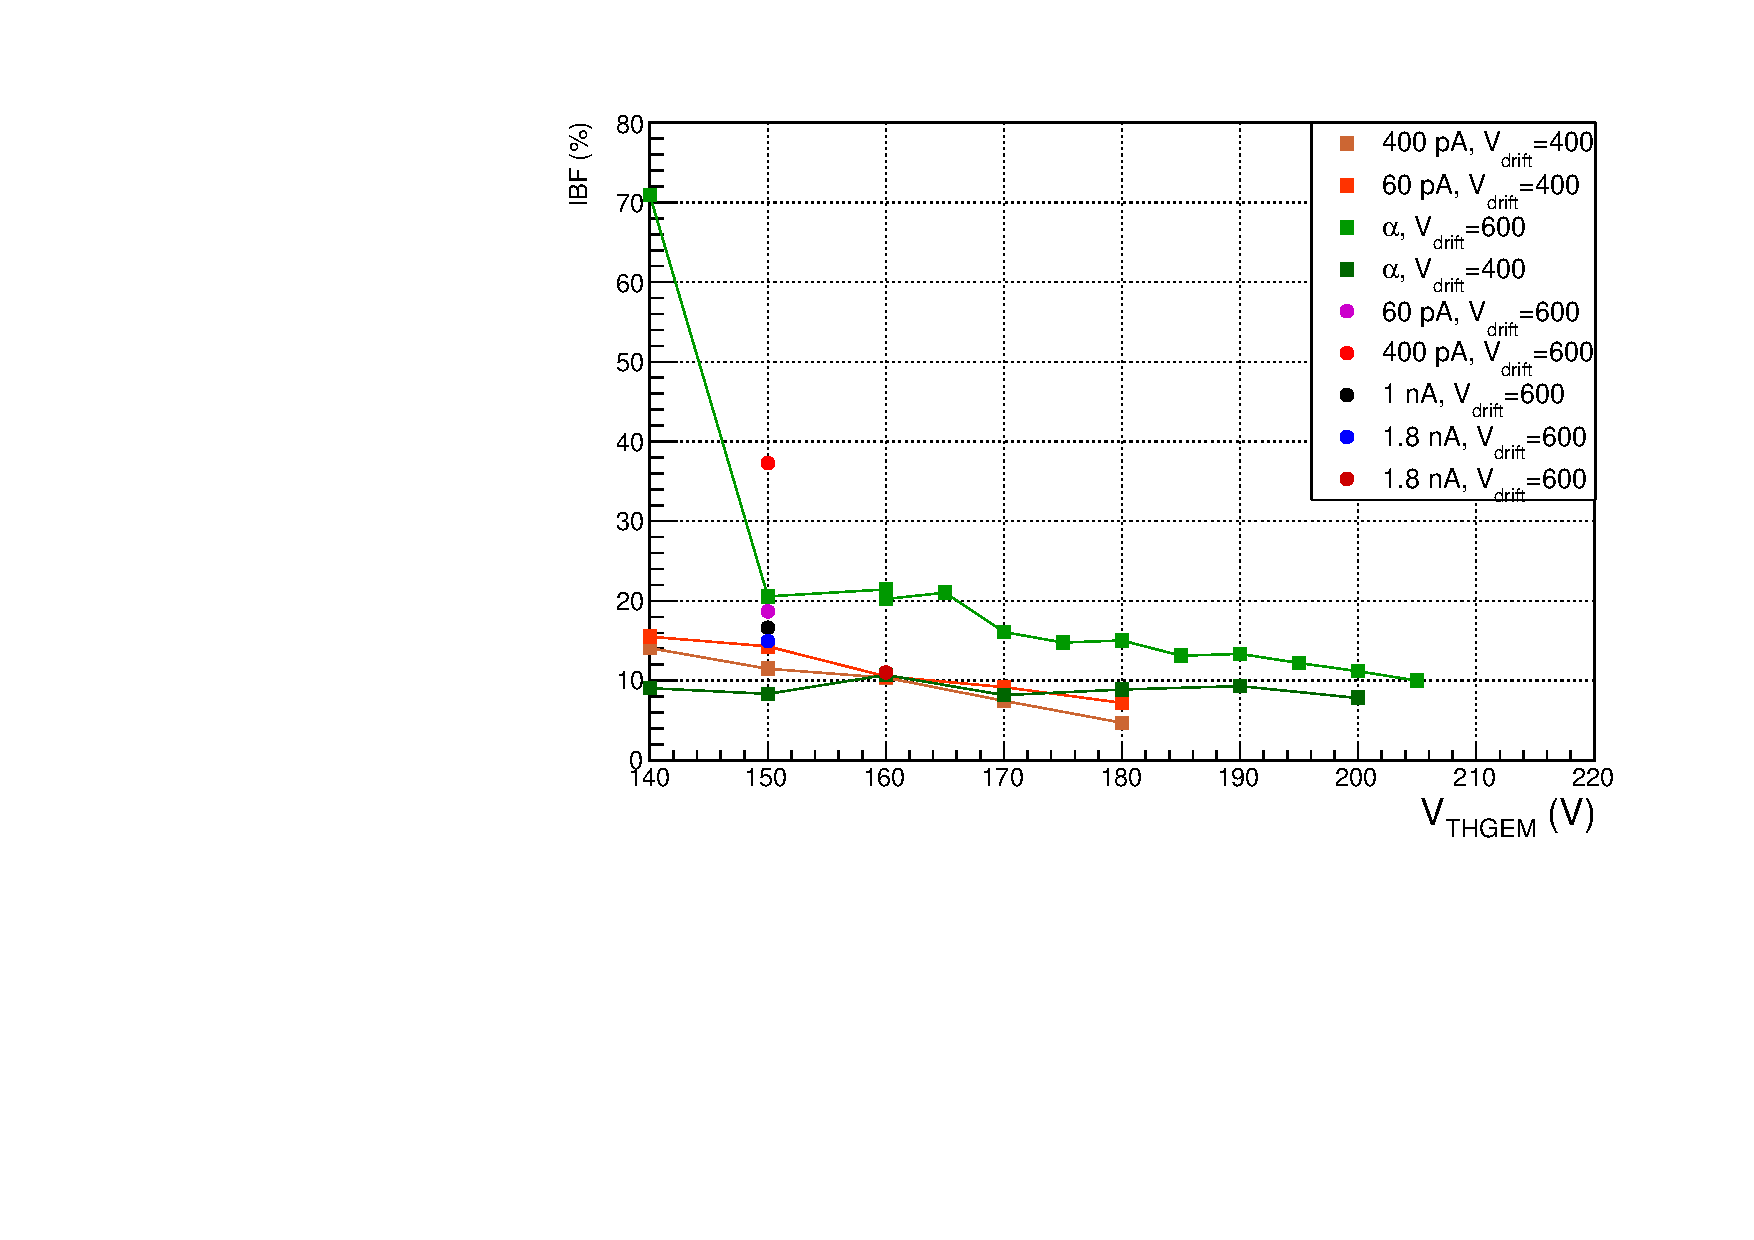
\includegraphics[width=0.96\textwidth]{Immagini/IBFvsTHGEM_beam_alpha_zoom.pdf}}
	\caption{Ion backflows evaluated for FULL THGEM as a function of \Vthgem{} at 60 pA, 400 pA, 1 nA, 1.8 and with alpha source.}
	\label{fig:IBFvsTHGEM_beam_alpha}
\end{figure}



In figure~\ref{fig:IBFvsInd_beam.pdf} it is visible as IBF value is very different in FULL and ROW THGEM, respectly 20\% and 60\%. Another difference is IBF behavoir, IBF is constant for FULL THGEM and it decrease for ROW THGEM. IBF as a function of \Vind{} is not dependent from pressure and it decrease increasing beam current.

\begin{figure}[htbp]
	\centering
	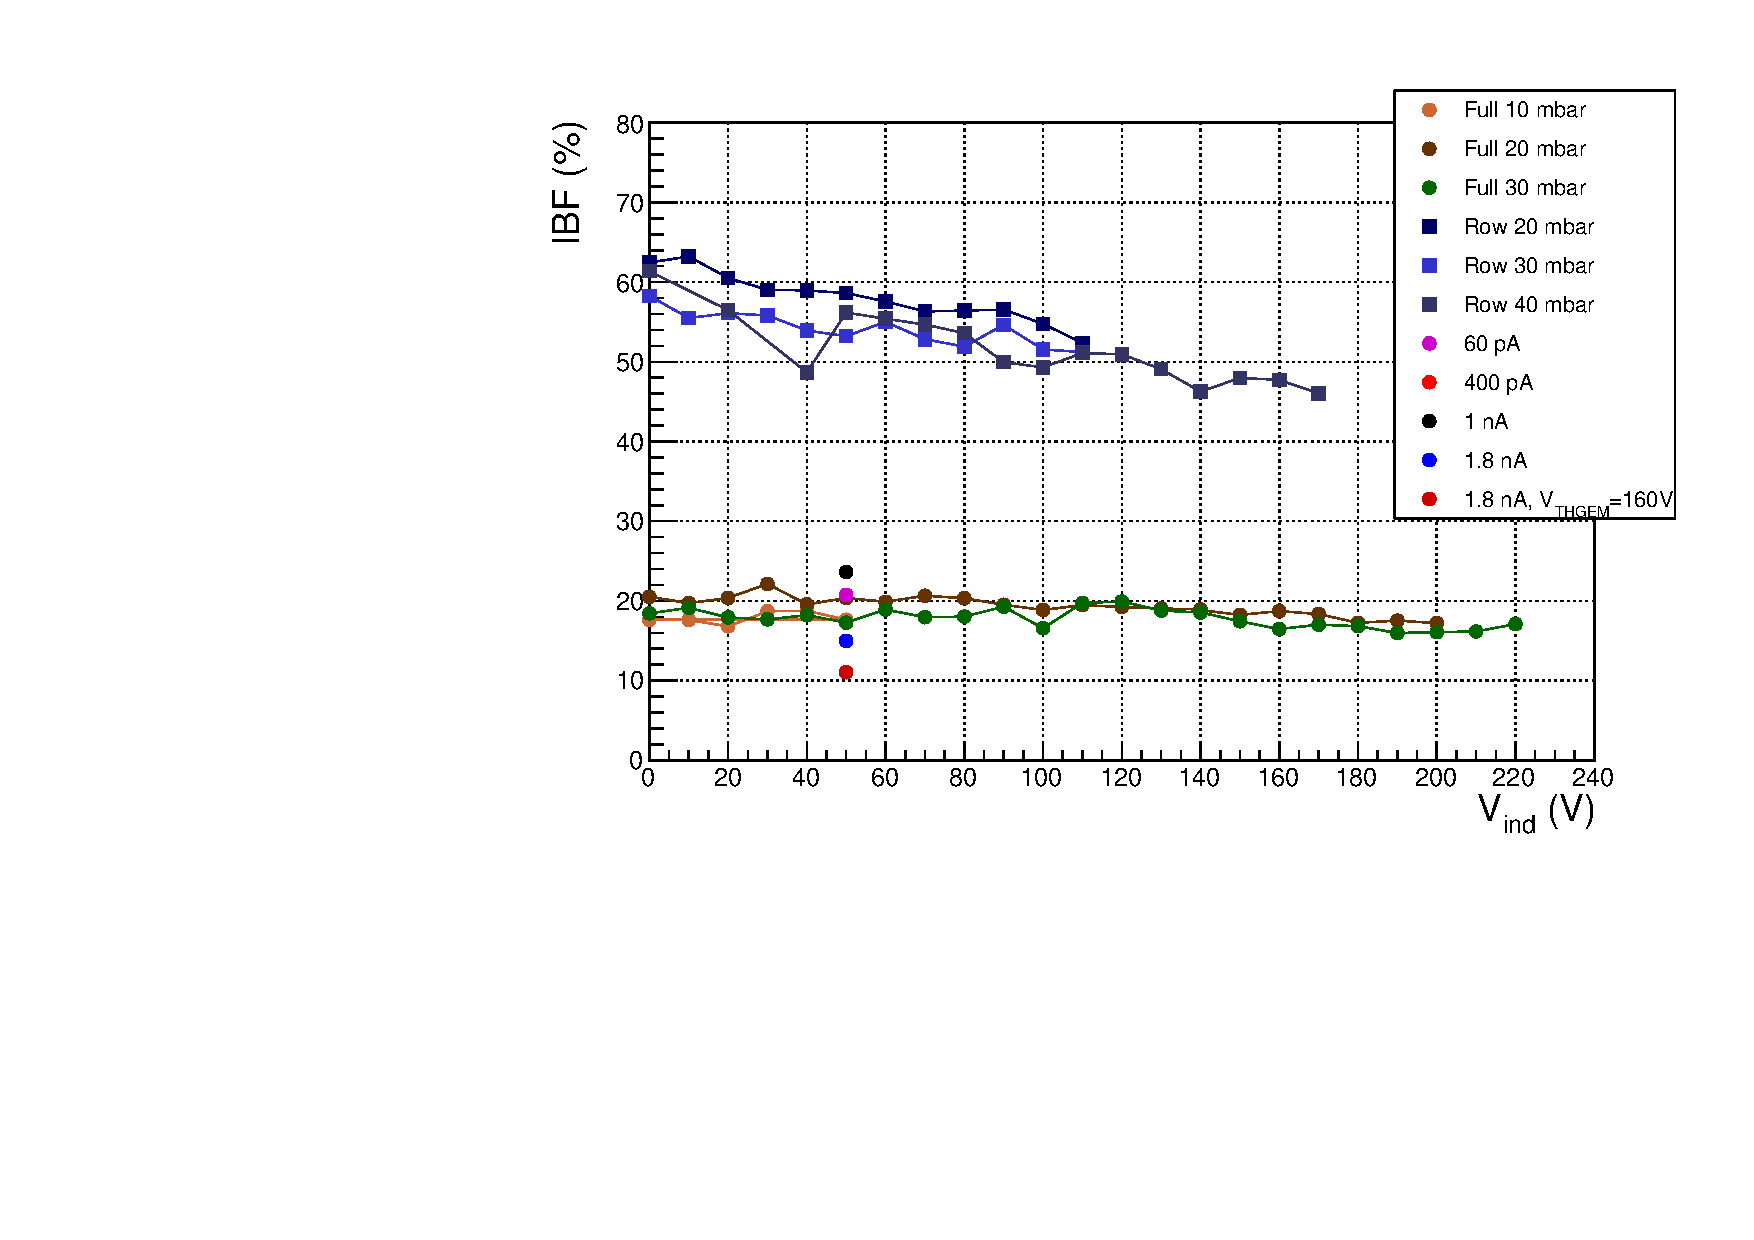
\includegraphics[width=\textwidth]{Immagini/IBFvsInd_beam.pdf}
	\caption{Ion backflows evaluated for FULL THGEM as a function of \Vind{} at 60 pA, 400 pA, 1 nA, 1.8 nA and with alpha source.}
	\label{fig:IBFvsInd_beam.pdf}
\end{figure}


\subsubsection{Beam Scan}

In figure~\ref{fig:IbeamScan_THGEM10_10mbar_average} the measured currents were plotted at the increasing of beam current. We expected a linear behavior instead we found an exponential one. This behavior can be explained because the point at 60 pA and 400 pA have different conditions from tre others. To measure at 1 nA and 1.8 nA a collimator was removed from beam line so the beam spot and its distribution i different.

\begin{figure}[htbp]
	\centering
	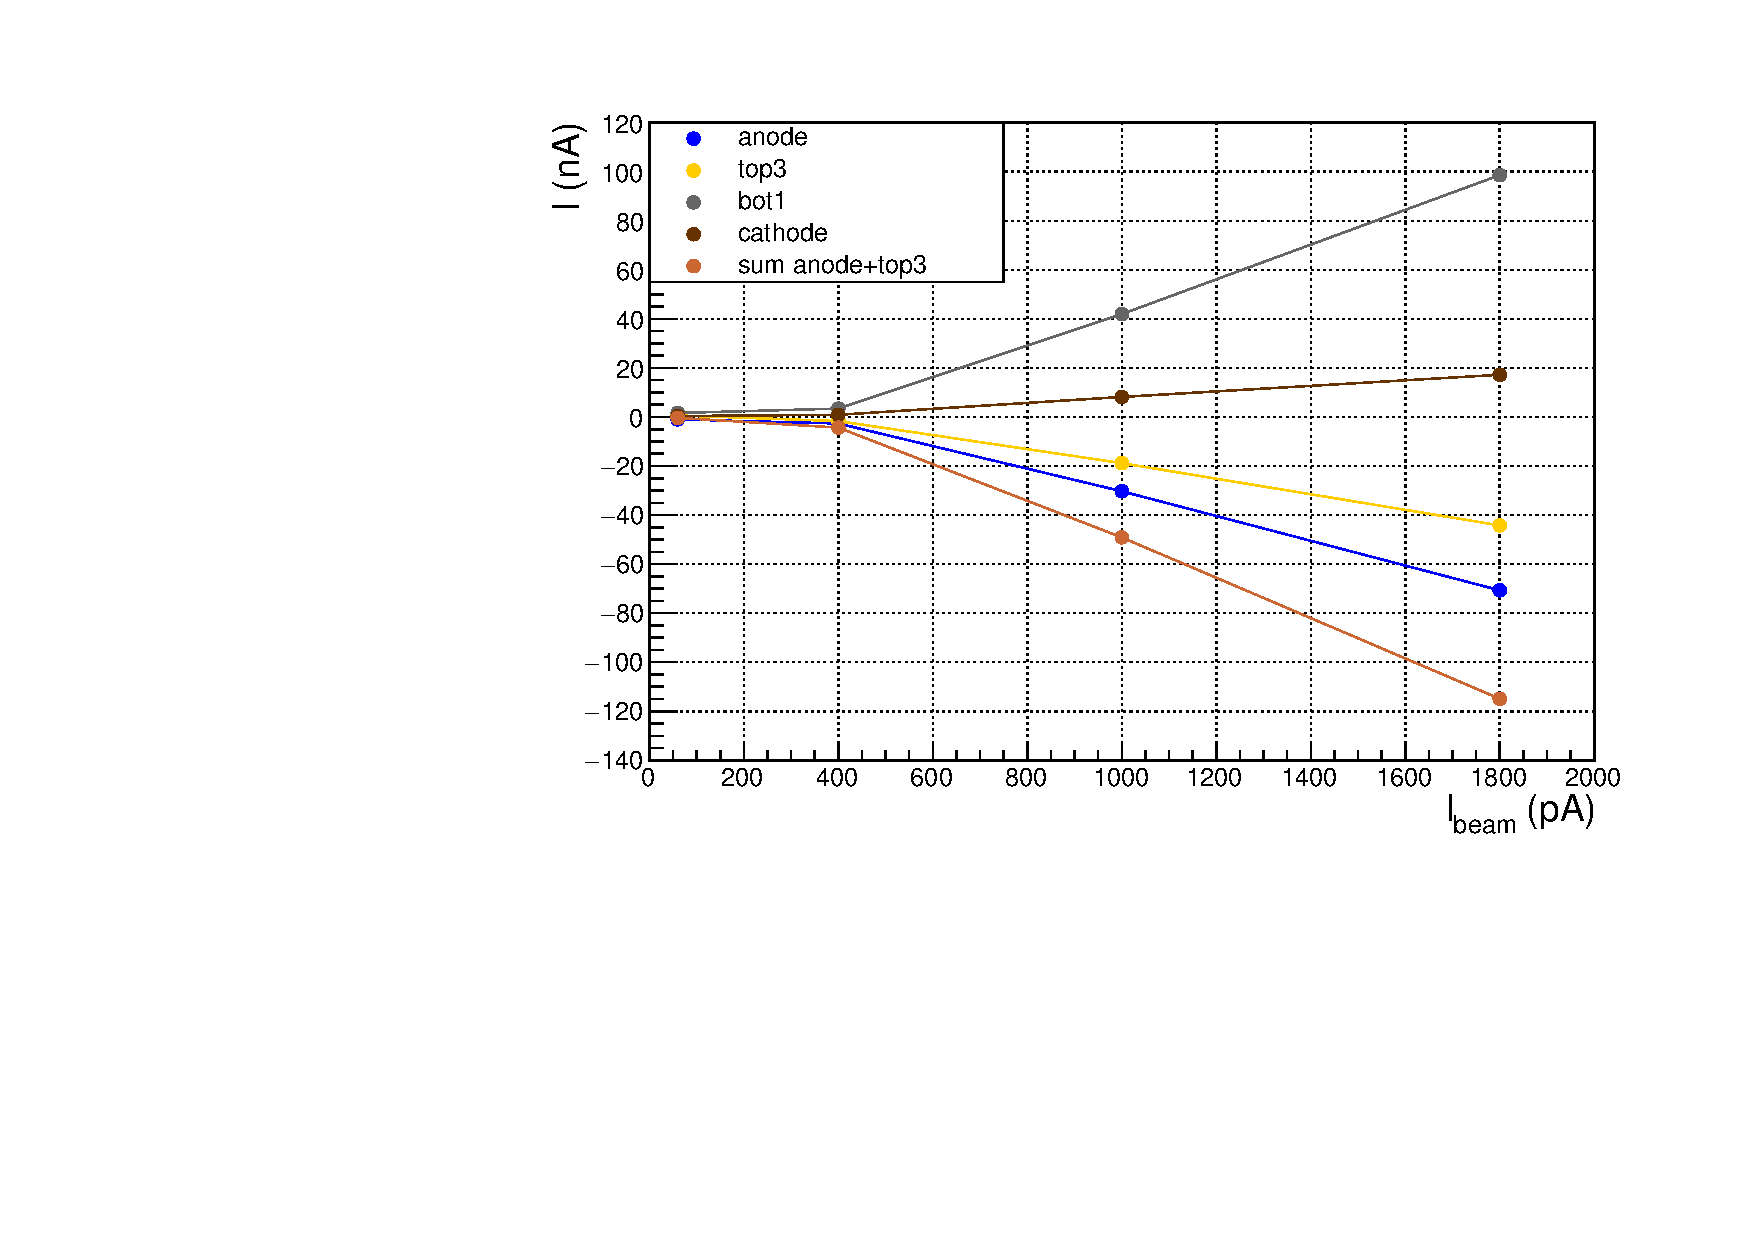
\includegraphics[width=\textwidth]{Immagini/IbeamScan_THGEM10_10mbar_average.pdf}
	\caption{Currents measured during the beam scan on the voltage across each FULL THGEM at 60 pA, at 400 pA, at 1 nA, at 1.8 nA.}
	\label{fig:IbeamScan_THGEM10_10mbar_average}
\end{figure}

%\section*{Notes}

%partiamo dalle full thgem:

%sulla parte di induzione: uno dei grafici con i quattro canali e la somma appropriata, incrocio fra corrente anodo e top3, regione di quasi plateau, poi la corrente aumenta, se avremo delle simulazione potremo corredare il discorso; obiettivo: cercare la regione di migliore funzionamento che dovrebbe essere quella del plateau



%sulla parte delle thgem: andamento esponenziale, si raggiunge il limite di scarica, non sappiamo se la scarica \E8 nelle thgem



%sulla parte di drift: variare la corrente tra catodo e bottom1; a 0 volt abbiamo una misura: o lo strumento segna zero ma non \E8 zerp 


%%descrizione delle varie pressioni: un grafico tenendo soltanto anodo a diverse pressioni, questo grafico non varia drammaticamente al variare della pressione; un altro grafico con l'induzione al variare della tensione delle thgem e/o del drift.



%%ion backflow: calcolare direttamente il valore in percentuale; unico grafico al variare delle pressioni; esso non dipende molto dall'induzione; esso dipende anche delle thgem (configurazione delle linee di forza); conclusione: 

%%fattore di moltiplicazione: inizialmente solo con le thgem piene;
%%poi thgem row e mostrare i tre grafici esemplificativi
%%induzione delle row thgem a 20 mbar \E8 pi\F9 bello;

%\subsection{ROW THGEM}

%%la drift \E8 da discutere: la loro geometria \E8 diversa: 5 fila isolate e proviamo a spiegare che a basse tensioni della drift, il campo elettrico delle thgem forma un imbuto pi\F9 largo, se vdrift aumenta la regione da cui le thgem raccolgono carica diminuisce

%%dalle row thgem ci aspettiamo meno corrente perch\E9 hanno meno buchi: invece di 143 file, ne hanno 5, quindi hanno il 3.5\% dei buchi rispetto a quelle piene. In prima approssimazione potremmo aspettarci che il valore della corrente scali allo stesso modo. 

%%ion backflow nelle row \E8 sistematicamente pi\F9 alto; vediamo se l'andamento \E8 simile; al variare dell'induzione diminuzione dell'IBF; 

%ricordarsi di fare la misura del drift delle row a 20 mbar
%ATTENZIONE: altri test tenendo i campi elettrici fissi
%Misura ad alta pressione con full thgem, misura ad altre pressione con row thgem e rifare i test cercando di mantenere i campi elettrici costanti (possibilmente con il drift a tensioni basse)



%\section{Conclusioni}




\end{document}
